\documentclass[a4paper,11pt]{article}
%\documentclass[a4paper,10pt,twocolumn]{article}
\usepackage[spanish]{babel}
\usepackage[utf8]{inputenc}
\usepackage[]{amsmath} %para embeber texto en math
%Para el manejo de gráficos .eps 
%\usepackage[dvips]{graphicx} 
\usepackage[pdftex]{graphicx}
%\usepackage{latexsym}
% Esto para gestión de archivos jpg
%\usepackage{graphicx} 
%
%Para que coloque las referencias a figuras y ecuaciones recuadradas y
%que haga el link a ellas tambi\'en
\usepackage{hyperref}
\hypersetup{colorlinks=false}

\frenchspacing
\hyphenation{co-la-bo-ra-ci-on Che-ren-kov di-fe-ren-cias nues-tro 
e-xis-ten-tes in-te-rio-ri-zar-se Tie-rra la-bo-ra-to-rio ex-pe-ri-men-tos
re-so-na-do-res ac-tu-a-li-dad pos-te-rior}
\usepackage{vmargin}

\setpapersize{A4}
\setmargins{2.5cm}       % margen izquierdo
{1.5cm}                  % margen superior
{16.5cm}                 % anchura del texto
{23.42cm}                % altura del texto
{10pt}                   % altura de los encabezados
{1cm}                    % espacio entre el texto y los encabezados
{0pt}                    % altura del pie de página
{2cm}                    % espacio entre el texto y el pie de página

\graphicspath{ {media/} }

\begin{document}
\author{L. Horacio Arnaldi}
\title{Documentación del nuevo sistema de adquisición de datos del Proyecto
Latin American Giant Observatory (LAGO)}
\date{17 de septiembre de 2018}
\maketitle
\tableofcontents

\section{Control de versiones}
\begin{itemize}
\item v0.1 30/04/2018 Versión inicial
\item v0.2 06/08/2018 Revisión 0.2
\begin{itemize}
\item Nuevo hardware rp\_ctrl\_board
\item Nuevo modo de adquisición con muestra de rates en los canales
\end{itemize}
\begin{itemize}
\item v0.3 17/09/2018 Se agrega alguna descripción sobre el header de los nuevos archivos de
				datos.
\item Se agregan pasos para actualizar la carpeta \texttt{src/} desde el
				repositorio git.
\end{itemize}
\begin{itemize}
\item v0.4 09/11/2018 Se agregan más descripciones a la instalación del sistema
				NFS en el servidor y en el cliente.
\end{itemize}
\end{itemize}

\section{Introducción}
En este documento se detallan los pasos, configuraciones y/o instalaciones
necesarias para que funcione el nuevo sistema de adquisición de datos de LAGO en
la placa RedPitaya (RP).

\section{El ecosistema LAGO}
El ecosistema LAGO consiste en
\href{https://github.com/lagoprojectrp/lago\_ecosystem}{un repositorio git} que
contiene el código fuente, tanto \texttt{VHDL} como \texttt{C}, de los proyectos,
ip-cores, ejemplos de uso y pruebas en general realizados para el nuevo sistema de
adquisición de datos del Proyecto LAGO. 

El ecosistema trabaja con Vivado 2016.4
y todas las pruebas se hicieron hasta ahora en un sistema Linux 16.04.
  
El código es open-source con licencia 3-Clause BSD License.

\begin{figure}[!h]
  \centering
    \fbox{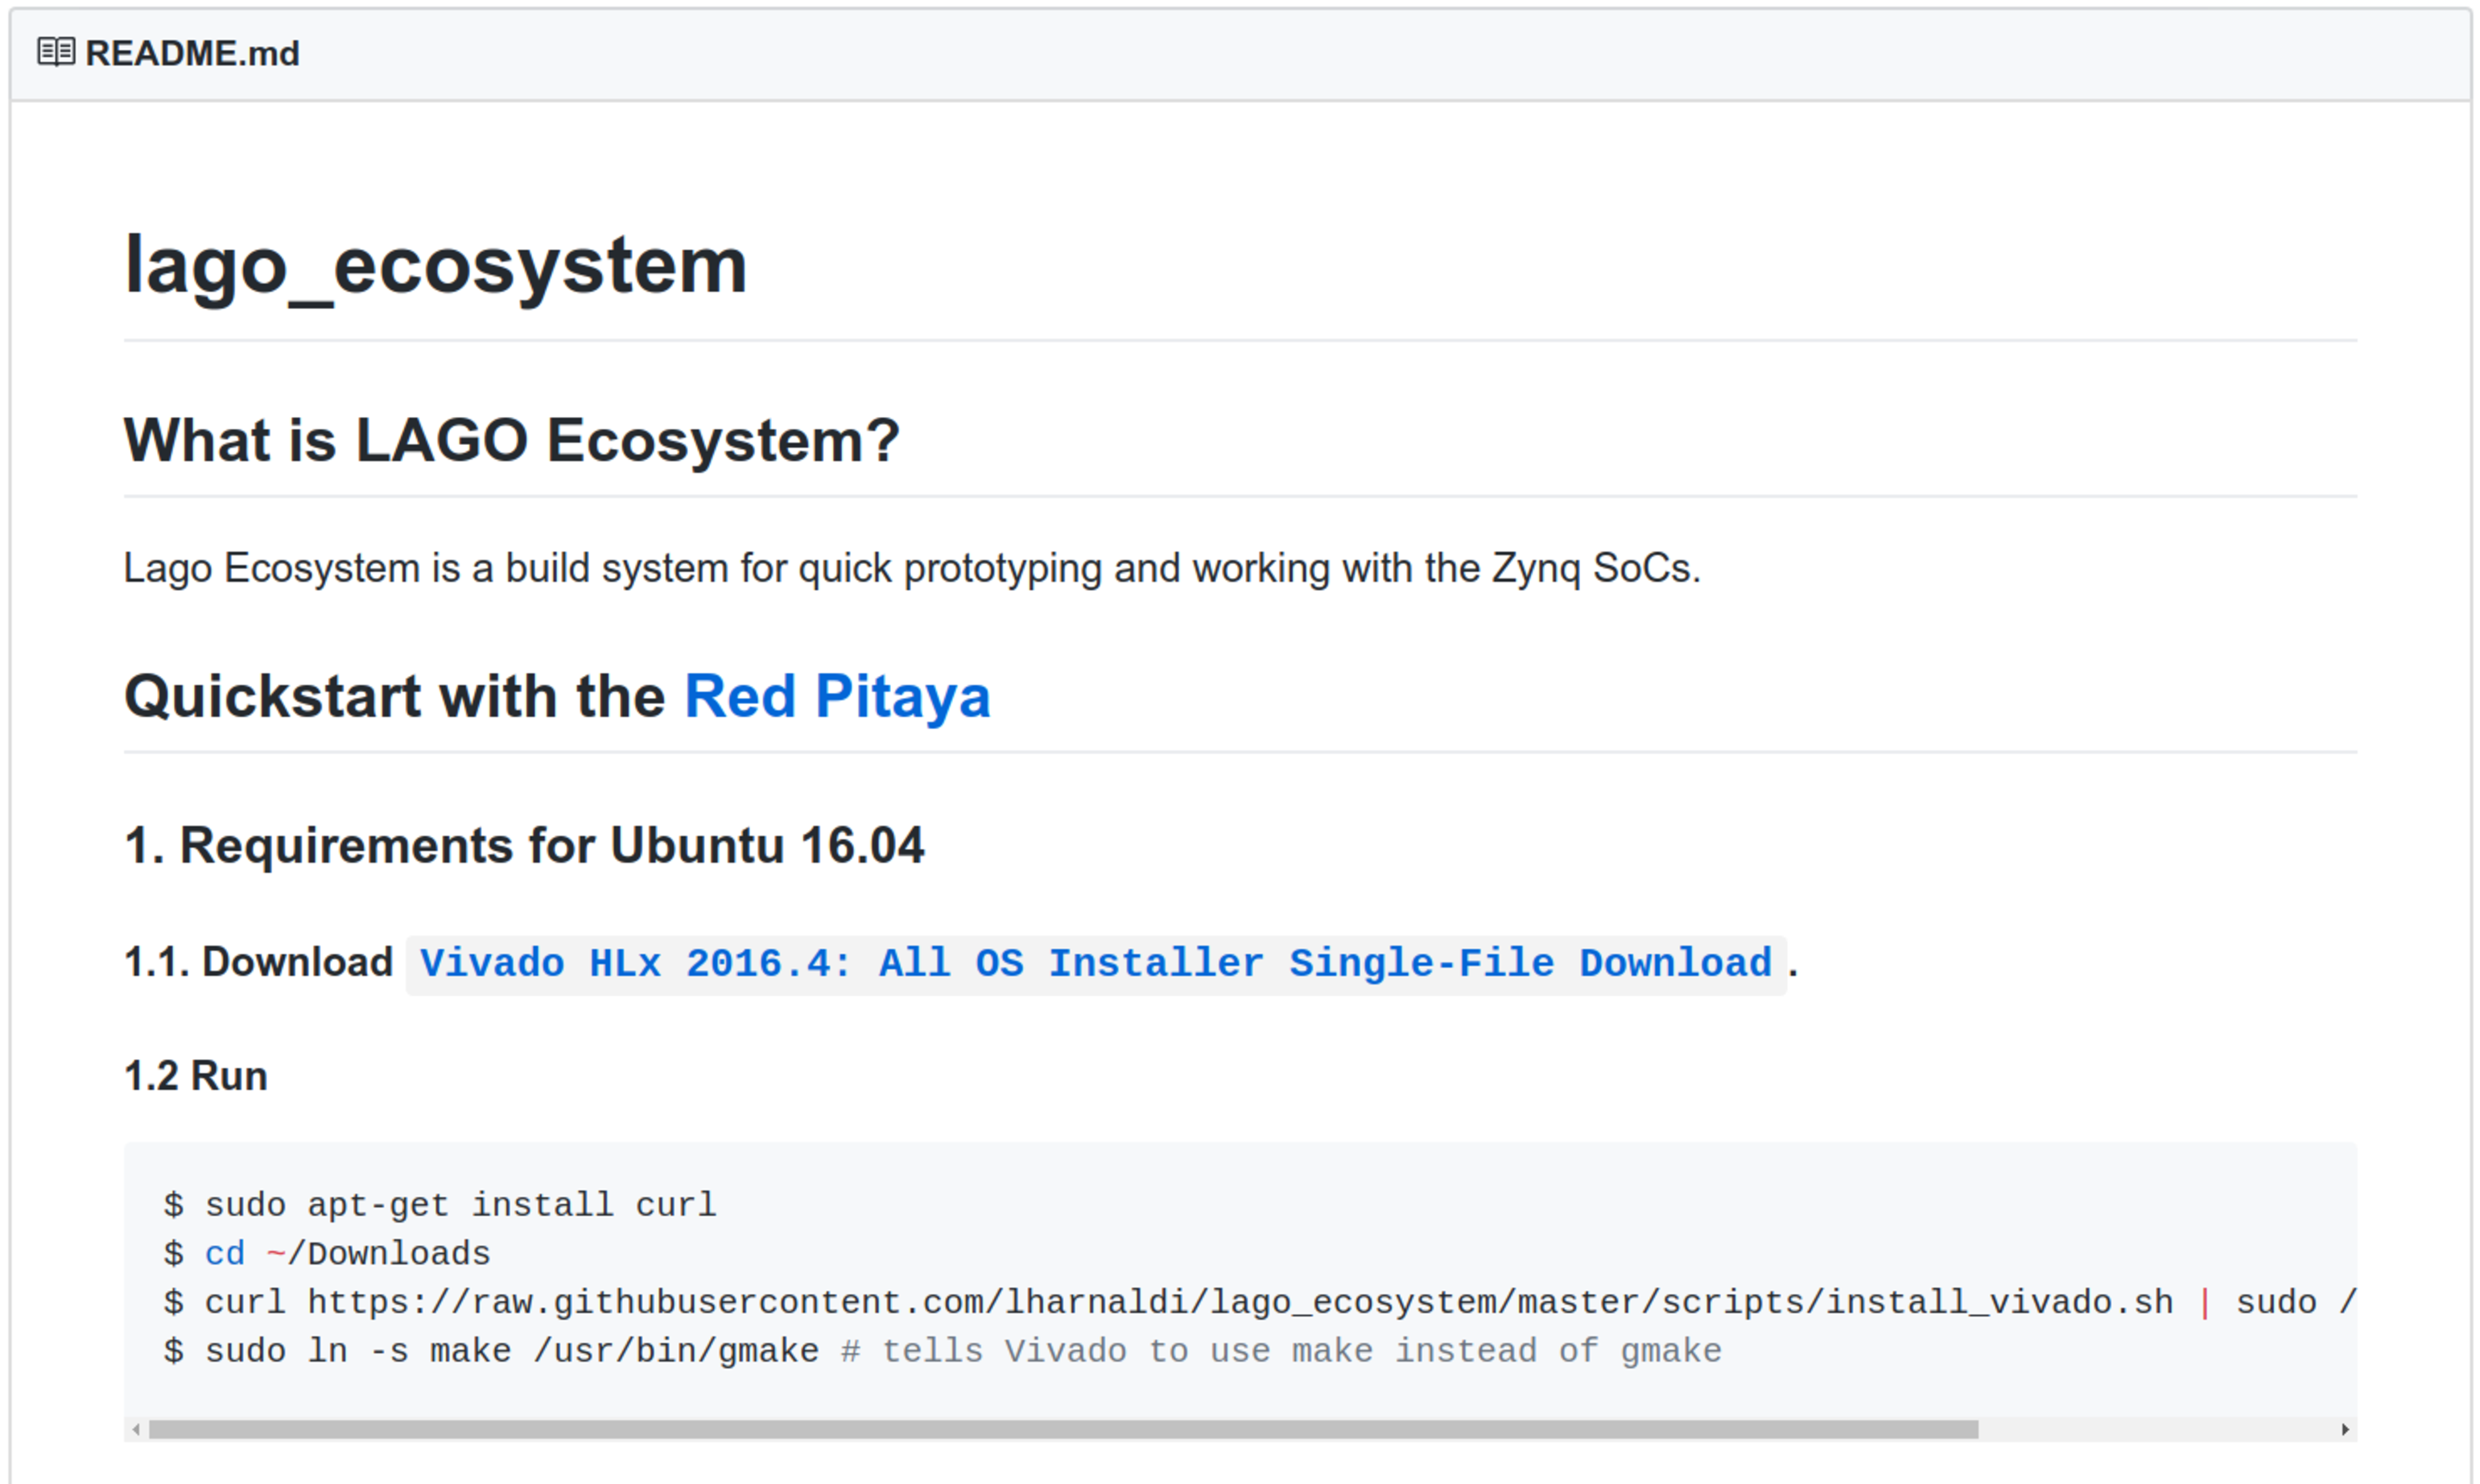
\includegraphics[height=10cm,width=16.5cm]{pag_lago_ecosystem}}
  \caption{Archivo README del ecosistema LAGO, tal como puede verse en el
repositorio git.}
  \label{fig:pag_ecosystem}
\end{figure}

\begin{itemize}
  \item Es una herramienta que facilita el descubrimiento, la
        experimentación, el aprendizaje, el desarrollo y el hecho de compartir una
        variedad de aplicaciones.
  \item Consiste en un sistema de directorios estructurado de acuerdo a los
        componentes software del sistema RedPitaya.
  \item Contiene librerías base que permiten hacer programas para controlar las
entradas/salidas analógicas, las entradas/salidas digitales, la comunicación
(I2C, SPI, UART) y otros.
  \item Sirve para programar y depurar código (C, Python, Matlab, VHDL,
        Verilog, etc.).
  \item Constituye una de las herramientas fundamentales en el proceso de
        desarrollo/modificación de nuevas aplicaciones.
  \item Contiene todo lo necesario para programar la FPGA y el procesador
        ARM.
  \item Se encuentra en un repositorio git para el control de versiones y
        cambios.
%  \item Se va a necesitar lo siguiente para construir los componentes:
%\begin{verbatim}
%  sudo apt-get install make curl xz-utils git
%  sudo apt-get install libssl-dev device-tree-compiler u-boot-tools
%\end{verbatim}
%      \item Xilinx Vivado 2016.4 FPGA development tools.
%      \item Linaro ARM toolchain para cross-compilar las aplicaciones Linux. Se
%            recomienda instalarlo en \texttt{/opt/linaro/} debido a que las
%            instrucciones del proceso de construcción lo buscan allí.

\end{itemize}

\section{Vivado}
Vivado es la herramienta que se utiliza para trabajar con la FPGA (PL, de
\texttt{programmable logic}) y el procesador ARM (PS, de \texttt{processing
system}). La Fig.
\ref{fig:bloques_vivado} muestra el nuevo sistema de adquisición 
implementado en bloques. Entre otras cosas, en
Vivado se pueden asignar las direcciones de memoria en las cuales encontraremos
a nuestros periféricos dentro del sistema Linux, tal como puede verse en la
Fig. \ref{fig:addr_editor}.

\begin{figure}[!h]
  \centering
    \fbox{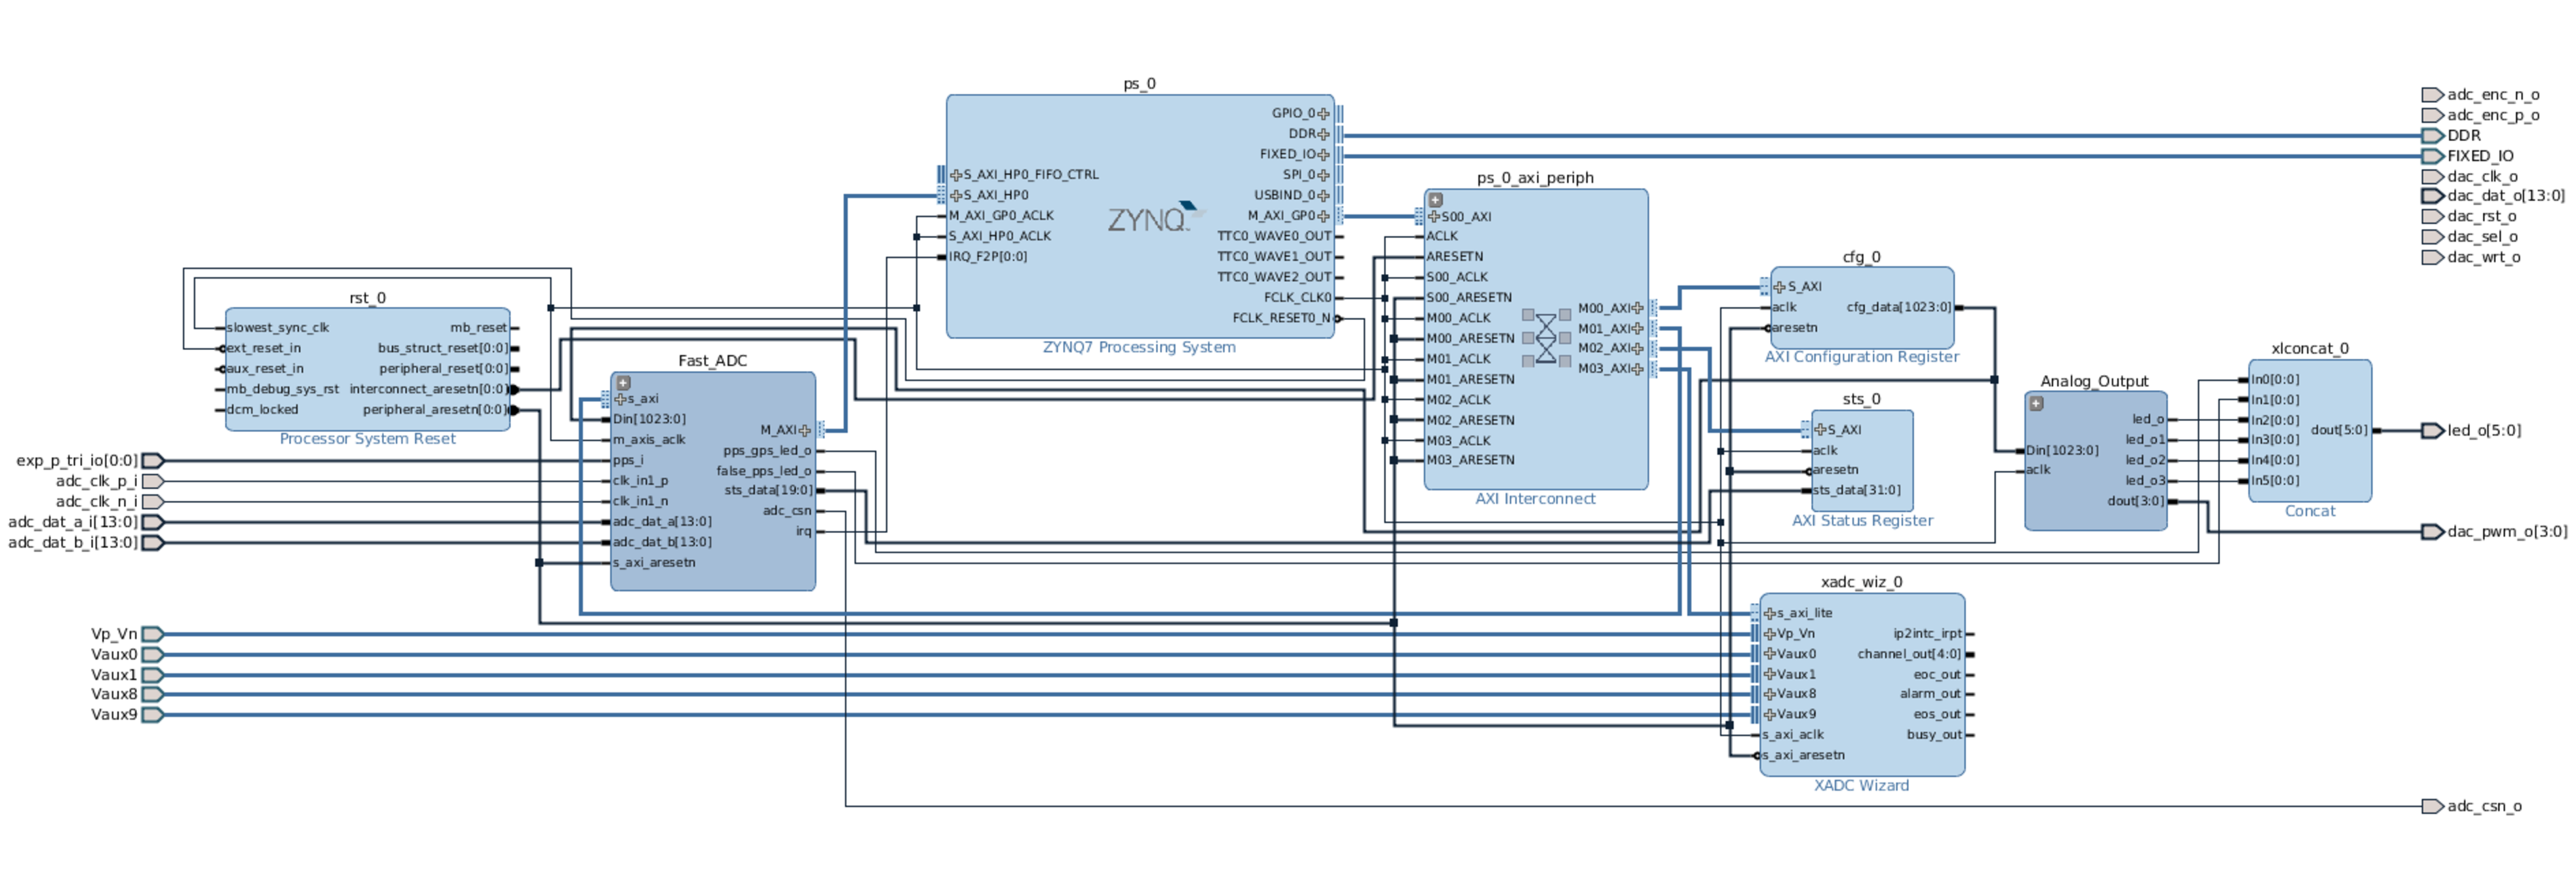
\includegraphics[height=6cm,width=16.5cm]{lago_sch}}
  \caption{Diagrama en bloques del sistema, tal como puede verse en Vivado.}
  \label{fig:bloques_vivado}
\end{figure}

\begin{figure}[!h]
  \centering
    \fbox{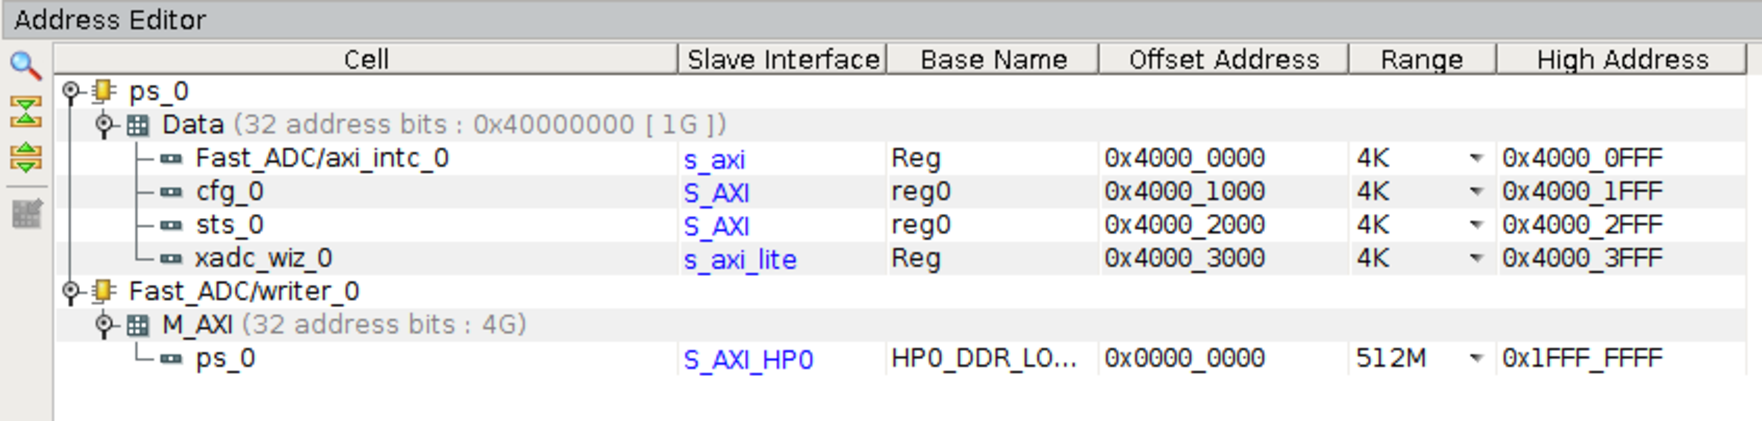
\includegraphics[height=4cm,width=16.5cm]{address_editor}}
  \caption{Address editor de Vivado. Se muestran las direcciones asignadas a los
bloques que componen el nuevo sistema de adquisición.}
  \label{fig:addr_editor}
\end{figure}

\section{Primeros pasos}

Se detallan los primeros pasos, tales como la instalación del sistema operativo
en la tarjeta SD y las configuraciones de proxy y/o red, necesarios para
empezar a trabajar con el nuevo sistema de adquisición de datos.

\noindent Algo muy importante de resaltar es la forma de apagar la RP. Resulta que si uno
simplemente desenchufa el cable de power de la RP para apagarlo, corre el
riesgo de dejar el sistema Linux instalado en la tarjeta SD inutilizable o
corrupto. Entonces, para realizar un apagado correcto del sistema, es necesario
ejecutar:

\begin{verbatim}
root@lago$ poweroff
\end{verbatim}

\noindent y esperar unos segundos antes de quitar la energía a la placa. De esta
forma nos aseguramos que la próxima vez que lo encendamos encontremos todo tal
y como lo habíamos dejado al apagarlo.

\subsection{Instalación del sistema LINUX en la tarjeta SD}

Para obtener la última versión del sitema operativo, dirigirse a la
\href{http://wiki.lagoproject.net/index.php?title=Main\_Page}{wiki del proyecto
LAGO}. En la sección \textit{\textbf{Electrónica}} se puede encontrar un link a
la página de descarga. 

El sistema Linux con el que se trabaja en la RP es un \textbf{Ubuntu 14.04.5
LTS},
distribución Trusty. La imagen se hizo para una tarjeta SD de $2\,\text{GB}$, por lo que
pesa unos $380\,\text{MB}$. Sin embargo, de ser necesario expandir la imagen se puede
consultar la sección \ref{subsub_expansion_sd}.
También se puede descargar la imagen directamente desde
\href{https://mega.nz/#!BxZgmLjY!I8BuaMg53Kzo\_eZQKRjOMfJlu95qR2zWT\_BbRXjgNVQ}{acá}.   

\noindent Para saber qué nombre le asignó el sistema a nuestra tarjeta SD una
vez que la conectamos a la PC, ejecutar:
\begin{verbatim}
lsblk
\end{verbatim}
\noindent con ese comando se puede saber si nuestra tarjeta SD es, por ejemplo,
\texttt{/dev/sdb} o \texttt{/dev/sdc}.

\noindent Una vez descargada la última versión de la distribución, ejecutamos:

\begin{verbatim}
sudo gzip -dc lago_linux_OS_stable_v1_0.gz | sudo dd bs=4M of=/dev/sdb
\end{verbatim}

\noindent y tendremos nuestra tarjeta SD lista para ser usada en la RP.

\subsection{Inicio del sistema}

Para conectarnos a la RP podemos usar la conexión por consola serie (puerto
micro-USB) o la conexión Ethernet.

\subsubsection{Conexión por consola (micro-USB)}

La conexión por puerto serie es independiente de la conexión Ethernet. Se debe
usar un cable con conector micro-USB para conectar la computadora con la
RedPitaya. Este puerto se usa generalmente cuando se necesita hacer debugging o
hacer pruebas en general. Es un puerto más lento que Ethernet, por lo que es de
uso secundario dentro de LAGO. 

La configuración del puerto serie para la
conexión está dada en la tabla \ref{table:uart}. Para conectarse desde una PC se
puede utilizar \texttt{minicom}\cite{bibMinicom}.

\begin{table}[!t]
\renewcommand{\arraystretch}{1.3}
\caption{Parámetros de configuración del puerto serie}
\label{table:uart}
\centering
\begin{tabular}{|l|p{2.0cm}|}
\hline
\bf{Parámetro} & \bf{Valor}\\
\hline\hline
Speed        & 115200\\
Data bits    & 8\\
Stop bits    & 1\\
Parity       & none\\
Flow control & none\\
\hline
\end{tabular}
\end{table}

\subsubsection{Conexión por Ethernet}

Para encontrar nuestra RP en la red de nuestra Universidad/Institución
ejecutamos en nuestra PC:

\begin{verbatim}
sudo nmap -sP 10.73.22.1-254
\end{verbatim}

\noindent Este comando indica que se busque en nuestra red, que es 10.73.22.0 y que busque
entre el rango de direcciones 1 a 254. De esa forma nos aseguramos de buscar en
toda nuestra red. Así, obtendremos una salida con la siguiente apariencia
(además de otras):
 
\begin{verbatim}
Nmap scan report for 10.73.22.195
Host is up (-0.100s latency).
MAC Address: 00:26:32:F0:16:62 (Instrumentation Technologies d.d.)
\end{verbatim}

\noindent De acuerdo a la salida del comando \texttt{nmap}, hemos hallado nuestra RP en la
dirección \texttt{10.73.22.195}. Lo importante acá es hallar la salida que se
corresponda con \texttt{Instrumentation Technologies}. Otro dato adicional que
obtenemos es la MAC address de nuestro dispositivo, que en este caso es
\texttt{00:26:32:F0:16:62}. 

\noindent Una vez que nos conectamos, hacemos el login (user: \texttt{root}, pass: \texttt{escondido})
\begin{verbatim}
lago login: 
Password: 
\end{verbatim}

\noindent Luego de esto estaremos adentro del sistema:

\begin{verbatim}
Welcome to Ubuntu 14.04.5 LTS (GNU/Linux 4.6.0-xilinx armv7l)

 * Documentation:  https://help.ubuntu.com/

The programs included with the Ubuntu system are free software;
the exact distribution terms for each program are described in the
individual files in /usr/share/doc/*/copyright.

Ubuntu comes with ABSOLUTELY NO WARRANTY, to the extent permitted by
applicable law.

root@lago:~# 

\end{verbatim}

\noindent Puede que queramos hacer los cambios necesarios en la interface de red antes de
arrancar el sistema en la RP. Para eso y antes de retirar la tarjeta SD de la
PC, la montamos y vamos a modificar el archivo
\texttt{/etc/network/interfaces.d/eth0} para poder acceder por \texttt{ssh} a una ip fija
que conozcamos. Por defecto Trusty trae habilitado el servidor ssh, pero la
configuración de la interface Ethernet viene puesta por DHCP. Debemos cambiar
esa configuración por defecto y colocar una ip que conozcamos. Esto también nos
servirá en caso de querer conectarnos directamente desde nuestra PC a la RP a
través de un cable UTP.

\noindent Cambiar el archivo \texttt{/etc/network/interfaces.d/eth0}. Donde
dice:

\begin{verbatim}
 iface eth0 inet dhcp
\end{verbatim}

\noindent cambiar por:

\begin{verbatim}
 iface eth0 inet static
 address 10.73.22.220 
 netmask 255.255.255.0
 gateway 10.73.22.2
\end{verbatim}

\noindent donde las direcciones de red, netmask y gateway dependerán de las 
respectivas configuraciones de red que se tengan en sus
Universidades/Instituciones.

\noindent Si es necesario configurar el proxy de la red, creamos el siguiente archivo:

\begin{verbatim}
vim /etc/apt/apt.conf.d/80proxy
\end{verbatim}

\noindent y agregamos (por ejemplo, para el proxy en Bariloche):

\begin{verbatim}
 Acquire::http::proxy "http://proxy.cab.cnea.gov.ar:3128/";
\end{verbatim}

\noindent podemos agregar servidores DNS también (aunque esto no es ya necesario
debido a que el sistema se autoconfigura una vez iniciado). 

Para agregar servidores DNS editamos el archivo \texttt{/etc/resolv.conf} y
colocamos, por ejemplo:

\begin{verbatim}
 nameserver 10.73.2.100
 nameserver 10.73.2.102
 nameserver 8.8.8.8
\end{verbatim}

\noindent Con esto tendremos nuestro sistema listo para inetractuar con nosotros
y los detectores.

\subsection{Automatización del tiempo}
Como sabemos, en LAGO es necesario tener un registro estable y confiable del
tiempo. Para lograr que nuestro sistema se autoconfigure correctamente con el
tiempo local deberemos instalar el paquete NTP. De esta forma siempre tendremos
un sistema sincronizado y actualizado respecto del tiempo. Instalar NTP:

\begin{verbatim}
apt install ntp
\end{verbatim}

\noindent Eso es todo, la RP ahora está sincronizando su tiempo con los servidores NTP. Por
defecto usa servidores NTP que generalmente están lejos de nuestra locación.
Esto es malo para la precisión del tiempo. Así que primero debemos ir a la página
\texttt{pool.ntp.org} y buscar una ubicación lo más cerca posible a nosotros.
Para configurar los servidores NTP,
abrimos el archivo de configuración ntp.

\begin{verbatim}
vim /etc/ntp.conf
\end{verbatim}

\noindent y encontramos las líneas que comiencen con ``servidor''. Reemplazamos esas líneas
por líneas con servidores de \texttt{pool.ntp.org}. En nuestro caso (Bariloche)
la configuración se ve así:

\begin{verbatim}
 server 0.south-america.pool.ntp.org
 server 1.south-america.pool.ntp.org
 server 2.south-america.pool.ntp.org
 server 3.south-america.pool.ntp.org
\end{verbatim}

\noindent Ahora debemos reiniciar el servicio NTP:

\begin{verbatim}
/etc/init.d/ntp restart
\end{verbatim}

\noindent Luego tenemos el comando para verificar si el tiempo se está
sincronizando correctamente. Para enumerar los servidores NTP con los que la RP está
sincronizando:

\begin{verbatim}
ntpq -pn
\end{verbatim}

\subsection{Instalación de dependencias}

La imagen para la tarjeta SD tiene instalados la mayoría de los paquetes
necesarios para que todo funcione desde el principio, sin embargo, aquí se
indican las dependencias.

\noindent Dependencias a instalar para que funcione el nuevo sistema de
adquisición:

\begin{verbatim}
apt update
apt install i2c-tools libi2c-dev python-smbus build-essential
\end{verbatim}

\subsection{Expansión del sistema de archivos}\label{subsub_expansion_sd}
Va a ocurrir en ocasiones que nosotros contamos con una tarjeta SD de mayor
tamaño que la imagen que descargamos para LAGO. Para verificar que estemos
utilizando toda la extensión de nuestra tarjeta SD, ejecutamos: 

\begin{verbatim}
root@lago:~/src# df -h
Filesystem      Size  Used Avail Use% Mounted on
/dev/root       1.8G  630M  1.1G  38% /
devtmpfs        224M  4.0K  224M   1% /dev
none            4.0K     0  4.0K   0% /sys/fs/cgroup
none             47M  188K   47M   1% /run
none            5.0M     0  5.0M   0% /run/lock
none            233M     0  233M   0% /run/shm
none            100M     0  100M   0% /run/user
/dev/mmcblk0p1   12M  6.3M  5.7M  53% /boot
root@lago:~/src# 

\end{verbatim}

\noindent si el caso es que necesitamos extender el tamaño del sistema de
archivos, deberemos seguir los siguientes pasos: 
\textbf{NOTA:} Estos pasos se hacen con la Redpitaya encendida y el sistema ya
iniciado.

\noindent Para que se disponga de la totalidad del espacio de la SD hay que ejecutar
\begin{itemize}
\item Borrar la segunda partición
\begin{verbatim}
fdisk /dev/mmcblk0
\end{verbatim}
Presionar las siguientes teclas en orden:
d 2 para borrar,
n p 2 Enter Enter para re-crear.

\item Reboot e ingresar:
\begin{verbatim}
 resize2fs /dev/mmcblk0p2
\end{verbatim}

\end{itemize}

\noindent Con eso tenemos el sistema en toda la SD. Para que los cambios surtan
efecto, hacer un reboot con: 
\begin{verbatim}
shutdown -r now
\end{verbatim}

\section{Trabajando con el código}

En la implementación del nuevo sistema de adquisición para LAGO se intentó
mantener la mayor compatibilidad posible con lo que hoy en día tenemos
funcionando. Sin embargo, existen diferencias obvias debido al cambio de
plataforma, como por ejemplo, que ahora se tienen dos canales en
lugar de los tres originales. El código es similar en su
funcionamiento y comandos a lo que ya tenemos funcionando. Así, por
ejemplo, para ver el estado de los registros es:

\begin{verbatim}
root@lago:~/src# ./lago -a
#Trigger Level Ch1 = 8190
#Trigger Level Ch2 = 8190
#High Voltage 1    = 0 
#High Voltage 2    = 0
#Trigger Scaler 1  = 1
#Trigger Scaler 2  = 1
#No GPS device is present or enabled

Status from registers complete!
\end{verbatim}

\noindent Para ver las opciones disponibles:
\begin{verbatim}
root@lago:~/src# ./lago -h

	The LAGO ACQUA suite
	Data acquisition system for the LAGO BRC electronic
	(c) 2012-Today, The LAGO Project, http://lagoproject.org
	(c) 2012, LabDPR, http://labdpr.cab.cnea.gov.ar

	The LAGO Project, lago@lagoproject.org

	DPR Lab. 2018
	H. Arnaldi, lharnaldi@gmail.com
	X. Bertou, bertou@gmail.com
	LAGO v2r0 comms soft

Usage: ./lago <action> <register> <value> [options]

	Actions:
	-a				Get all registers status
	-s				Set registers
	-f				Start DAQ and save data to file
	-o				Start DAQ and send data to stdout
	-g				Get GPS data
	-t				Get Pressure and Temperature data
	-i				Initialise registers to default values
	-x				Read the voltage in the XADC channels
	-v				Show DAQ version

	Registers:
	t1, t2				Specify triggers 1 and 2
	sc1, sc2			Specify scaling factor 1 and 2
	hv1, hv2			Specify high voltages
	ov1, ov2, ov3, ov4		Specify output voltages

	Options:
	-f <filename>			Specify file name


root@lago:~/src# 

\end{verbatim}

\noindent Para configurar un nivel de trigger:
\begin{verbatim}
root@lago:~/src# ./lago -s t1 300
Complete. Data written: 0x0000012c
root@lago:~/src# 
\end{verbatim}

\noindent donde 300 es un valor en ADC. En este caso $300\,\text{ADC}$ se
corresponde con unos $36.6\,\text{mV}$, ya que la resolución del ADC es de 14
bits.

\subsection{Cambios en el código}
Hasta ahora se tenía las siguientes salidas en el archivo de datos generado:

\begin{verbatim}
# x r D2         34837
# x r D1         35641
\end{verbatim}

\noindent en este caso, $D1$ y $D2$ correspondían a constantes solicitadas al
sensor de presión y temperatura HP03 de HopeRF. Ahora esas constantes no son
necesarias, ya que con el nuevo sensor BMP180 o BMP280 se leen directamente los
valores de presión y temperatura.

Ahora, el archivo de datos generado por la RedPitaya entrega los siguientes
datos:

\begin{verbatim}
# r2 0
# r1 1
\end{verbatim}

\noindent $r1$ y $r2$ corresponden a los rates (o frecuencias) de pulsos que se
tiene en los canales 1 y 2, respectivamente.

En cualquier caso, antes de iniciar la toma de datos y una vez que se haya
instalado el sistema operativo en la tarjeta SD y se haya iniciado el sistema
por primera vez, lo que hay que hacer es actualizar la carpeta \texttt{src/} que
viene con la imagen original. 

Para actualizar esa carpeta se pueden hacer dos cosas:
\begin{enumerate}
				\item Instalar GIT en la RedPitaya y luego clonar el repositorio
								completo del ecosistema

								\href{https://github.com/lharnaldi/lago\_ecosystem}{https://github.com/lharnaldi/lago\_ecosystem} 

								Esto no es recomendable ya que el ecosistema LAGO contiene
								muchas otras cosas que no son necesarias para la adquisición de
								los datos, lo cual lleva a utilizar espacio en disco que podría
								usarse para datos dentro de la RedPitaya.
				\item Instalar GIT en otra PC, clonar el repositorio y luego copiar
								solamente la carpeta 

								\texttt{lago\_ecosystem/projects/lago\_v1\_1/src} 
								
								que está en el
								repositorio a la RedPitaya. Luego del copiado, ejecutar
								\texttt{make} en la RedPitaya, dentro de esa carpeta, para tener
								la última versión del código funcionando.
\end{enumerate}
\section{La placa RP\_CTRL\_BOARD v1r0}
Esta placa se desarrolló en Bariloche y trabaja con el software presente en el
directorio \texttt{projects/lago\_v1\_1} dentro del ecosistema de trabajo. Los
archivos Gerbers y los esquemas de construcción de esta placa, así como mayor
información sobre la misma se puede encontrar en la Wiki de lago.

\begin{figure}[!h]
  \centering
    \fbox{\includegraphics[height=7cm,width=10cm]{rp_ctrl_board}}
  \caption{Placa rp\_ctrl\_board v1r0. Esta versión incluye todo lo necesario
para hacer funcionar hasta dos detectores de LAGO a la vez. Además, incluye un
conector para adosar un ventilador de $12\,V$ al sistema y así poder enfriar el
procesador.}
  \label{fig:rp_ctrl_board_photo}
\end{figure}

\section{La placa Leopard v0.1}

Las pruebas iniciales de funcionamiento del sistema de adquisición de datos se
hicieron con la placa Leopard v0.1. Esta placa es un desarrollo de la gente de
Ecuador y permite proveer los voltajes necesarios para alimentar una base de
PMT. También permite monitorear la tensión aplicada al PMT, así como el sensor
de temperatura presente en la base. El sistema de adquisición está probado con
esta placa y es completamente funcional con ella.

\begin{figure}[!h]
  \centering
    \fbox{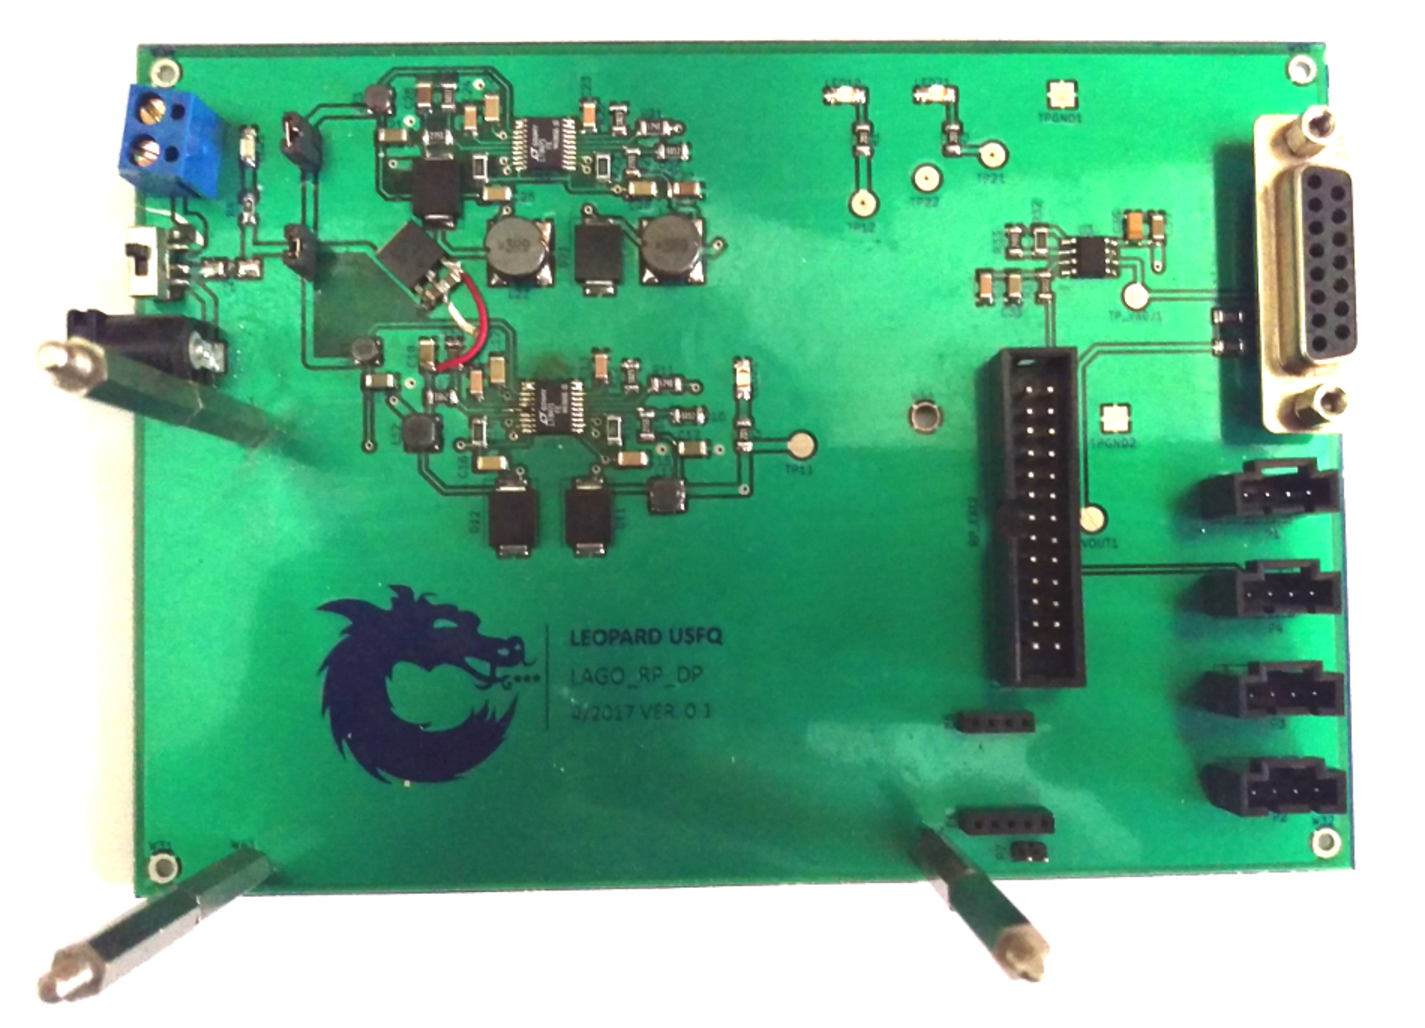
\includegraphics[height=7cm,width=10cm]{leopard_board_v0_1}}
  \caption{Placa Leopard v0.1. Esta versión tiene las salidas de +3.3V y -3.3V
para alimentar los sensores, además de la salida de +5V para alimentar la base
del PMT.}
  \label{fig:leopard_photo}
\end{figure}

\begin{figure}[!h]
  \centering
    \fbox{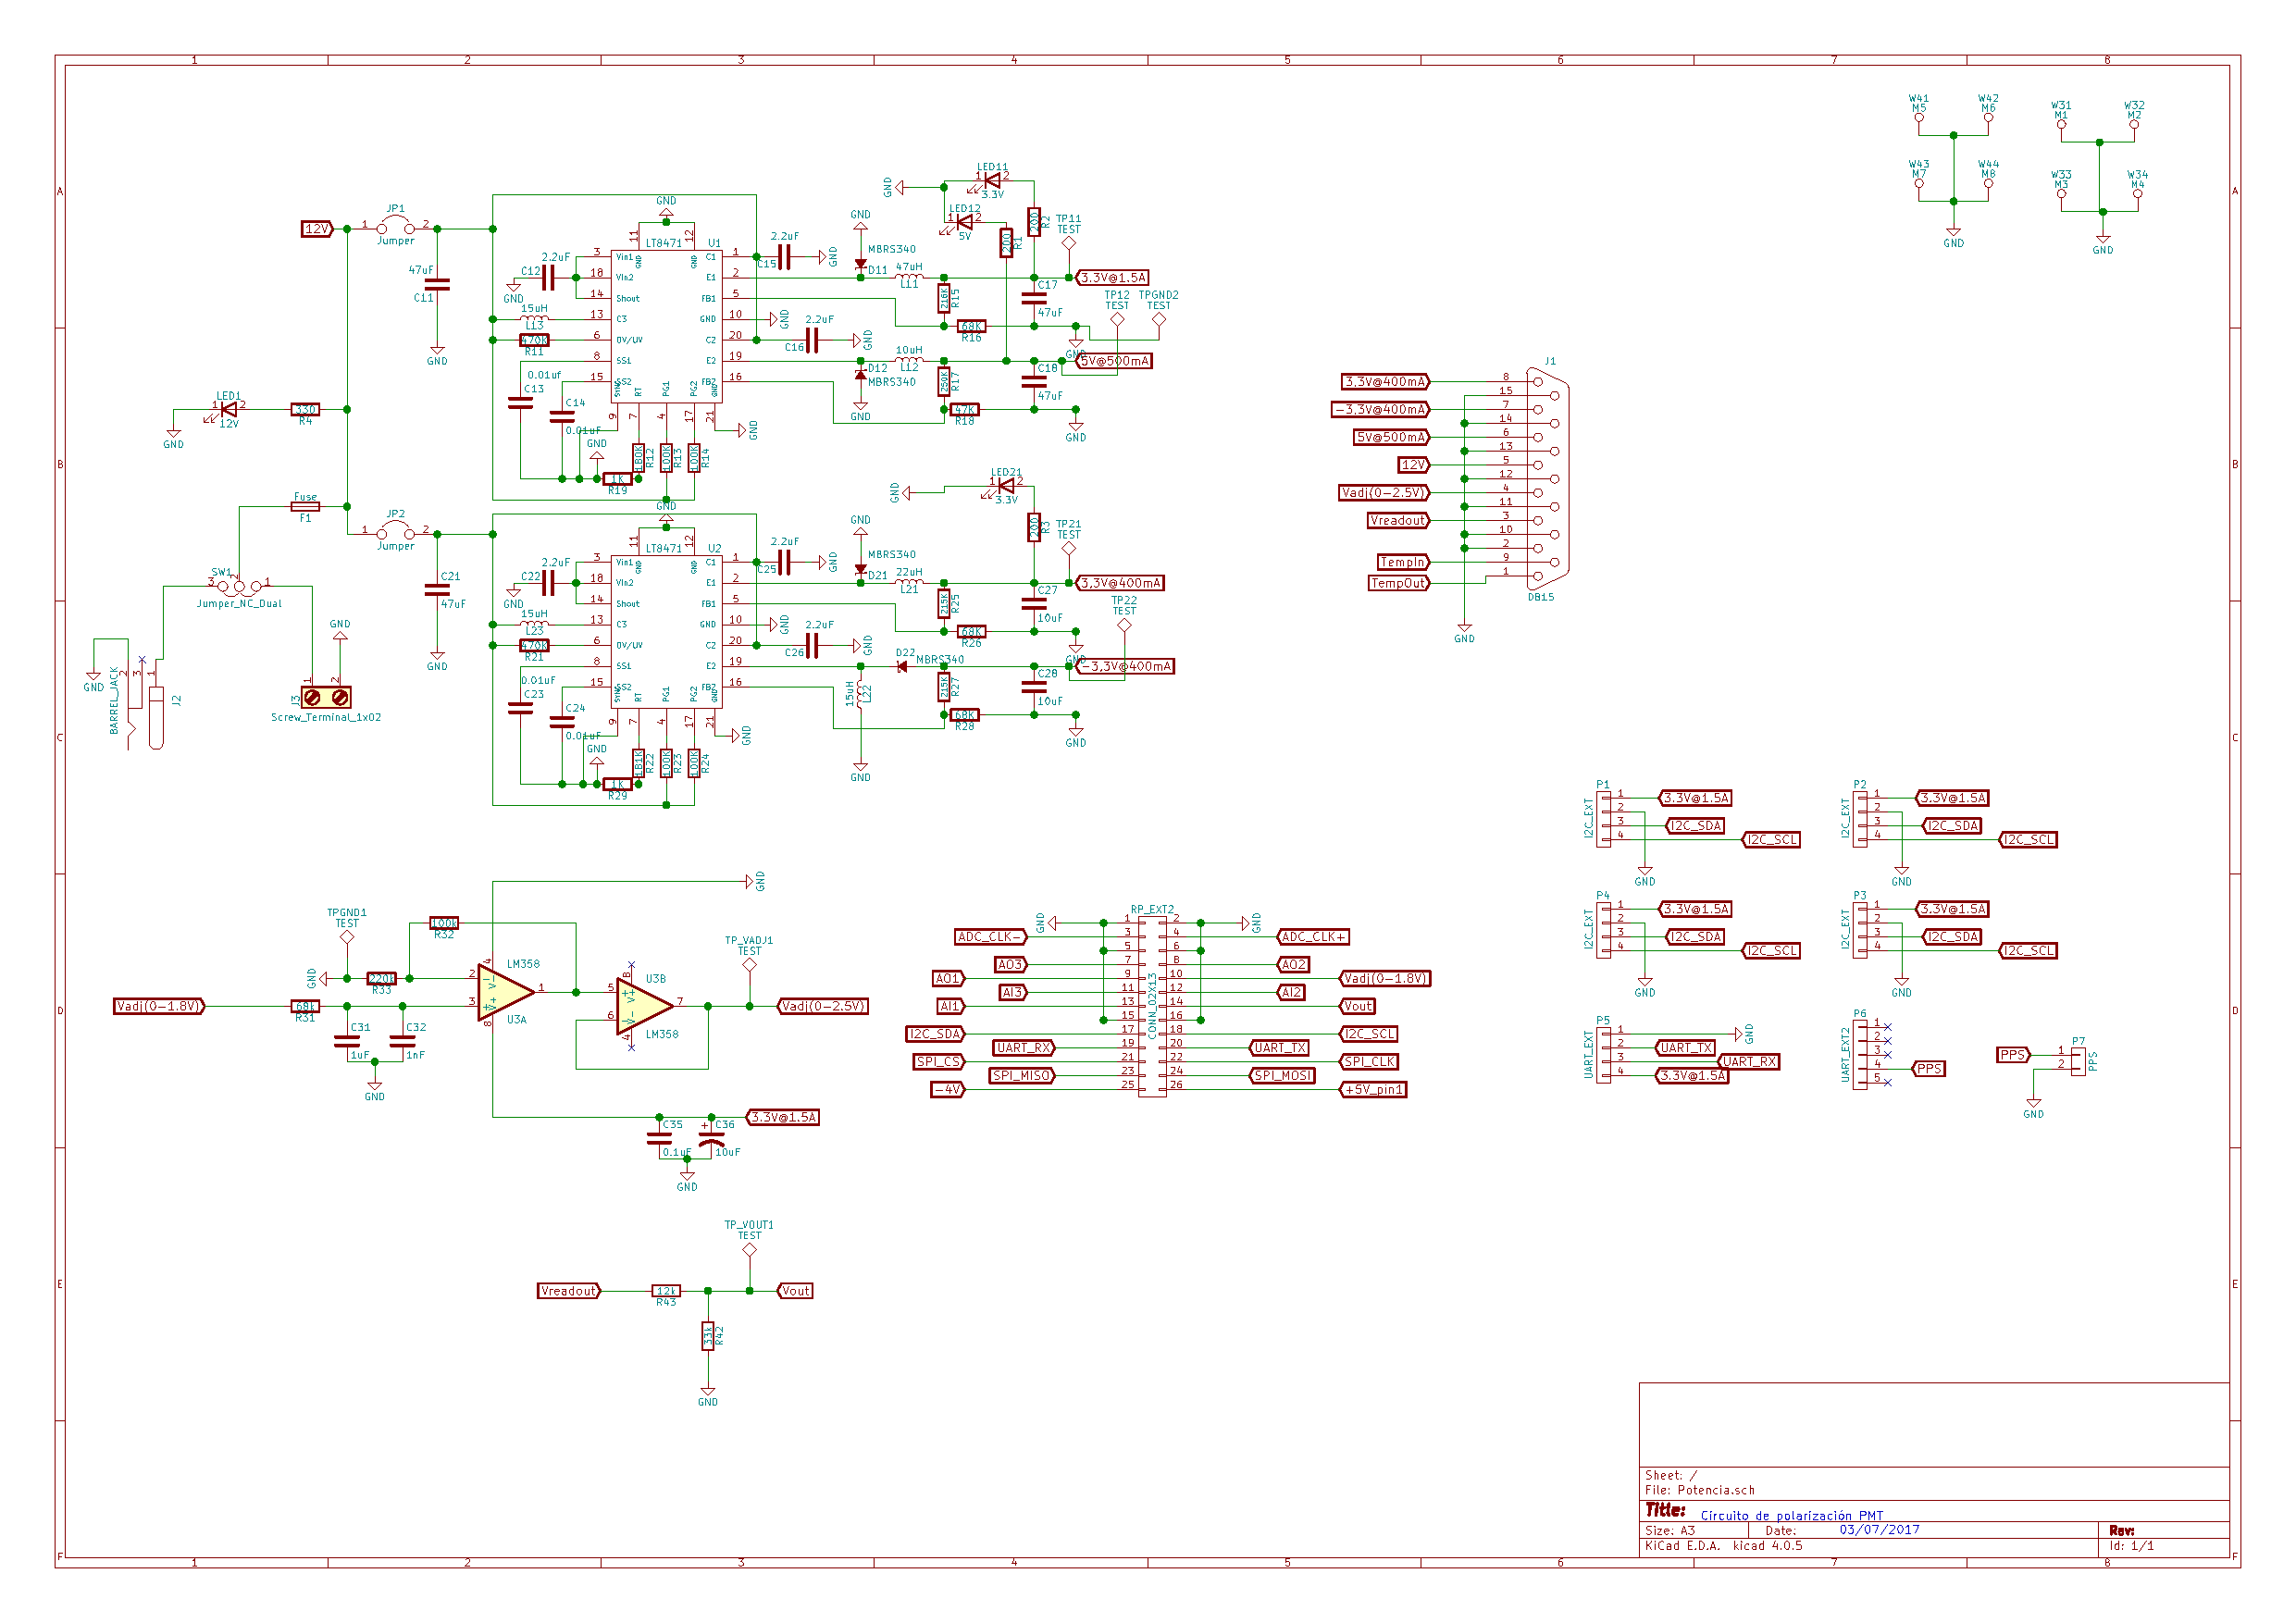
\includegraphics[height=10cm,width=16.5cm]{leopard_sch_v0_1}}
  \caption{Esquema de conexiones para la placa Leopard v0.1.}
  \label{fig:leopard_sch}
\end{figure}

\section{Sensores}
\subsection{GPS}
El GPS utilizado por el nuevo sistema de adquisición de datos es el GPSBee v1.2
\cite{bibGPSBee}.
En realidad, los comandos que entrega cualquier placa GPS actual son estándar y
se ajustan al protocolo NMEA. 
Se utiliza el estándar XBee para que sea compatible con muchos de los GPS que se
venden en la actualidad.

\begin{figure}[!h]
  \centering
    \fbox{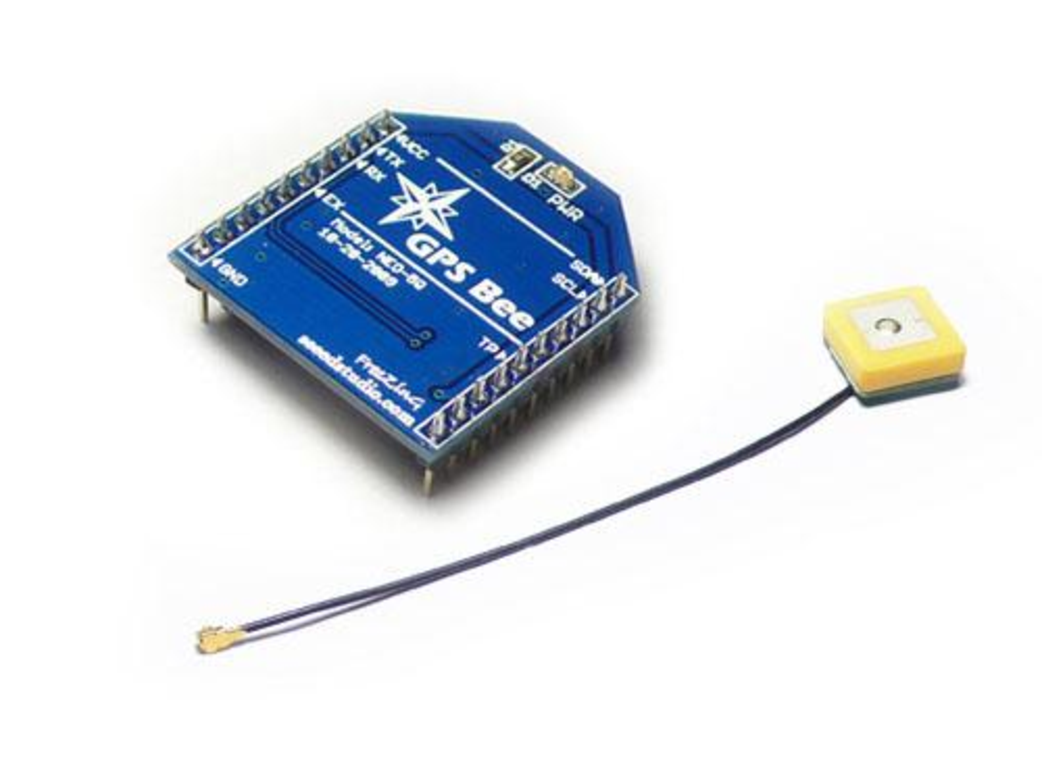
\includegraphics[height=6cm,width=6cm]{gpsbee}}
  \caption{Placa GPSBee en su versión v1.2. Esta placa es la que se utilizó en
las pruebas iniciales de funcionamiento del nuevo sistema de adquisición de
datos.}
  \label{fig:gpsbee}
\end{figure}

\subsubsection{Pruebas con el GPS}
Existe \href{https://github.com/lagoprojectrp/rp\_venusGps}{un repositorio
git} con el cual se pueden hacer pruebas de funcionamiento del GPS adosado a la
RP. Este es el resultado de correr el programa luego de compilarlo en la RP:
\begin{verbatim}
root@lago#./position_logger
-1.686342 -78.648947
-1.686345 -78.648957
-1.686348 -78.648962
-1.686355 -78.648970
-1.686360 -78.648975
-1.686365 -78.648982
-1.686370 -78.648990
-1.686375 -78.648995
-1.686378 -78.649003
-1.686382 -78.649012
-1.686387 -78.649015
\end{verbatim}

\subsection{Sensor de presión y temperatura}

\begin{figure}[!h]
  \centering
    \fbox{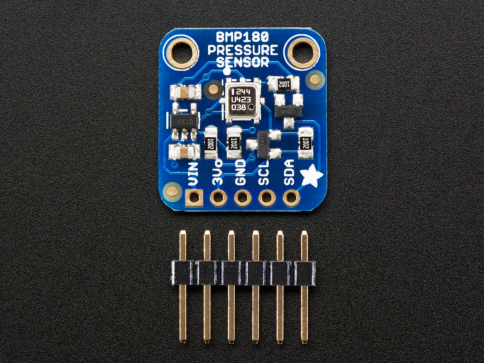
\includegraphics[height=6cm,width=8cm]{bmp180}}
  \caption{Placa BMP180. Esta placa es la que se utilizó en
las pruebas iniciales de funcionamiento del nuevo sistema de adquisición de
datos.}
  \label{fig:bmp180}
\end{figure}

Este sensor de bajo costo sirve para medir la presión barométrica, altitud y
temperatura. El sensor está soldado a un PCB con un regulador de 3.3V, un
circuito de cambio de niveles I2C y resistencias de pull-up en los pines I2C
\cite{bibBMP180}.

Esta placa se puede conectar a 5V. Se incluye un regulador de 3.3V y un circuito de
cambio de nivel I2C para que se pueda usar este sensor de forma segura con 5V de
lógica y potencia.

\subsubsection{Pruebas con el sensor de presión y temperatura}
Existe \href{https://github.com/lagoprojectrp/rp\_bmp180}{un repositorio
git} con el cual se pueden hacer pruebas de funcionamiento del sensor de PyT
adosado a la RP. Este es el resultado de correr el programa luego de compilarlo
en la RP:
\begin{verbatim}
root@lago# make
gcc -Wall -c bmp180.c -o bmp180.o -lm
gcc -Wall bmp180.o test.c -o test -lm
redpitaya> ls
bmp180.c  bmp180.h  bmp180.o  Makefile  test  test.c
redpitaya> ./test
Temperature = 23.2, Pressure = 73499, Altitude= 2627.0
Temperature = 23.2, Pressure = 73506, Altitude= 2626.6
Temperature = 23.1, Pressure = 73502, Altitude= 2627.3
Temperature = 23.1, Pressure = 73506, Altitude= 2626.6
Temperature = 23.1, Pressure = 73504, Altitude= 2626.6
Temperature = 23.1, Pressure = 73497, Altitude= 2626.8
Temperature = 23.1, Pressure = 73495, Altitude= 2627.4
Temperature = 23.1, Pressure = 73500, Altitude= 2627.0
Temperature = 23.1, Pressure = 73498, Altitude= 2626.7
\end{verbatim}

\section{NFS en RedPitaya}
\subsection{Montaje NFS}
\begin{itemize}
  \item NFS (sistema de archivos de red: \textbf{``Network File System''}) es un
        protocolo que permite acceso remoto a un sistema de archivos a
        través de la red.
  \item Todos los sistemas \textbf{Unix} pueden trabajar con este protocolo
  \item En un entorno de trabajo como LAGO se hace imprescindible disponer de
        un servicio que permita el acceso seguro a archivos remotos de forma
        trasparente.
  \item NFS trabaja bien para directorios que necesitan accederse de
        forma regular.
  \item NFS proporciona este servicio siguiendo la estructura
        cliente-servidor.
  \item El servidor NFS comparte una serie de directorios
        seleccionados con unas condiciones de seguridad concretas.
  \item El cliente NFS, si está autorizado para ello, puede ``montar''
        dichos directorios en su propio sistema de archivos pudiendo acceder
        a los archivos como si fueran locales.
  \item El montaje lo puede realizar en secuencia de arranque del equipo o
        cuando lo necesite.
\end{itemize}

\subsection{Prerequisitos}
\begin{itemize}
  \item Vamos a configurar el uso compartido de directorios entre dos
        dispositivos con Linux (PC y RedPitaya).
  \item Cada uno de estos dispositivos tendrá que tener una cuenta
        configurada con privilegios sudo.
  \item Vamos a hacer referencia al servidor que se va a compartir sus
        directorios como el \textbf{host} y el dispositivo que va a montar estos
        directorios como \textbf{cliente}. Para nuestro caso, el host es la PC y
        el cliente es la RedPitaya.
  \item Con el fin de demostrar la instalación, se van a utilizar las
        siguientes direcciones IP para el host y el cliente:
\begin{verbatim}
host: 192.168.0.112 
cliente: 192.168.0.111
\end{verbatim}
        \textbf{Se deben sustituir estos valores por los adecuados para sus
        host y cliente.}
\end{itemize}

\subsection{Descarga e instalación de componentes (servidor)}
\begin{itemize}
\item Antes de empezar, necesitamos instalar los componentes necesarios en
      ambos, el cliente y el servidor.
\item En el \textbf{host} necesitamos instalar el paquete
\texttt{nfs-kernel-server}, el cual nos permitirá compartir nuestros
directorios.
\begin{verbatim}
sudo apt-get update
sudo apt-get install nfs-kernel-server
\end{verbatim}
\end{itemize}

\subsection{Descarga e instalación de componentes (cliente)}
\begin{itemize}
\item En el \textbf{cliente} necesitamos instalar el paquete
            \texttt{nfs-common}, el cual permite tener la funcionalidad de NFS
            sin necesidad de incluir los componentes del servidor.
            directorios.
\begin{verbatim}
sudo apt-get update
sudo apt-get install nfs-common

\end{verbatim}
\end{itemize}

\subsection{El servidor NFS}
\subsubsection{Crear el directorio compartido}
En este caso, nos gustaría hacer que el directorio \texttt{/var/nfs} fuera
accesibles al cliente; por lo tanto  debemos ``exportarlo'' en el servidor.

Cuando un cliente accede a un recurso compartido de NFS, sucede normalmente como
el usuario \textbf{nobody}. 
%Generalmente el directorio /home no es propiedad de nadie (y no lo recomiendo
%cambiar su propiedad a nadie!), porque si queremos leer y escribir en /home,
%decimos al NFS que los accesos deben hacerse como root (si nuestra cuota/Inicio
%era de sólo lectura, esto no sería necesario). 

%No existe el directorio \texttt{/var/nfs}, así que debemos crearlo y cambiar sus
%propiedades de acceso.
%; en mis pruebas el usuario y grupo nobody tiene el ID el 99 en ambos mis
%sistemas de prueba de CentOS (servidor y cliente); Cuando traté de escribir a
%/var/nfs desde el cliente NFS, tengo un error de permiso denegado , así que
%hice un chmod 777 /var/nfs para que todo el mundo pudiera escribir en ese
%directorio.
    \begin{itemize}
      \item Creamos el directorio que vamos a compartir y le damos permisos
            adecuados:
\begin{verbatim}
sudo mkdir /var/nfs
sudo chown nobody:nogroup /var/nfs
\end{verbatim}
\end{itemize}

\subsubsection{Configurar \texttt{exports} de NFS}
\begin{itemize}
\item Ahora que tenemos nuestros directorios creados y asignados, podemos
      modificar el archivo de configuración de NFS para establecer la
      distribución de estos recursos.
\item Abrir el archivo \texttt{/etc/exports} con privilegios de root:
\begin{verbatim}
sudo vi /etc/exports
\end{verbatim}
\item Agregar la linea:
\begin{verbatim}
/var/nfs 192.168.0.111(rw,sync,no_subtree_check)
\end{verbatim}
\item A continuación, debe crear la tabla de NFS que mantiene las
exportaciones de sus acciones escribiendo:
\begin{verbatim}
sudo exportfs -a
\end{verbatim}
\item El servicio NFS no está funcionando realmente todavía. Puede
iniciarlo escribiendo:
\begin{verbatim}
sudo service nfs-kernel-server start
\end{verbatim}

\end{itemize}

\subsection{El cliente NFS}

Primero creamos el/los directorios donde queremos montar las acciones NFS, por
ejemplo:

%mkdir -p /mnt/nfs/home
\begin{verbatim}
mkdir -p /mnt/nfs/var/nfs
\end{verbatim}

Posteriormente, podremos montarlos (debemos hacerlo como root, o
escribiendo sudo delante si es un usuario con permisos):

\begin{itemize}
  \item Hay dos formas de hacer la configuración del montaje de recursos
        remotos:
        \begin{enumerate}
          \item Montar el directorio compartido solamente cuando se
                necesite.
          \item Hacer el que sistema monte el directorio remoto en el
                arranque.
        \end{enumerate}
\end{itemize}

\subsubsection{Montar el directorio remoto solo cuando se necesite}
\begin{itemize}
  \item Para eso ejecutar:
\begin{verbatim}
  mount -o nolock 192.168.0.112:/var/nfs /mnt
\end{verbatim}
\end{itemize}

\subsubsection{Montar el directorio remoto en el arranque del sistema}
\begin{itemize}
  \item Abrir el archivo:
\begin{verbatim}
sudo vim /etc/fstab
\end{verbatim}
\item En la parte inferior del archivo, vamos a añadir una línea:
\begin{verbatim}
192.168.0.112:/var/nfs /mnt/nfs/var/nfs  nfs  \\
rsize=8192,wsize=8192,timeo=14,intr
\end{verbatim}
%\\
%auto,noatime,nolock,bg,nfsvers=4,sec=krb5p,intr,tcp,actimeo=1800 0 0  
\end{itemize}

De esta forma, cuando se tomen datos con el sistema de adquisición, se podrá ir
guardando esos datos remotamente en el servidor.
Así, por ejemplo, para tomar y guardar los datos de forma remota:
\begin{verbatim}
./lago -f /mnt/nfs/var/nfs/gaga
\end{verbatim}

\section{Vivado: Instalación \& Licenciamiento}
\subsection{Introducción}

\subsubsection{Vivado como herramienta de desarrollos}
    \begin{itemize}
      \item Sirve para programar, depurar y simular código HDL (VHDL, Verilog e
incluso C) para la FPGA.
      \item Constituye una de las herramientas fundamentales en el proceso de
            desarrollo/modificación de nuevas aplicaciones.
      \item Permite trabajar con esquemas (bloques) y/o código HDL.
      \item Soporta todas las familias de FPGA de la serie Zync7000.
      \item Existe un sistema listo para usar dedicado a RedPitaya.
    \end{itemize}

\subsubsection{Página de descargas}
 Página de descargas: xilinx.com
  Vivado HLx Web Install Client
    Descargamos el cliente web ($\sim$\,80\,MB). Este cliente se encargará de
descargar e instalar todo lo necesario en nuestro sistema.
\begin{figure}[!h]
	\centering				
    \fbox{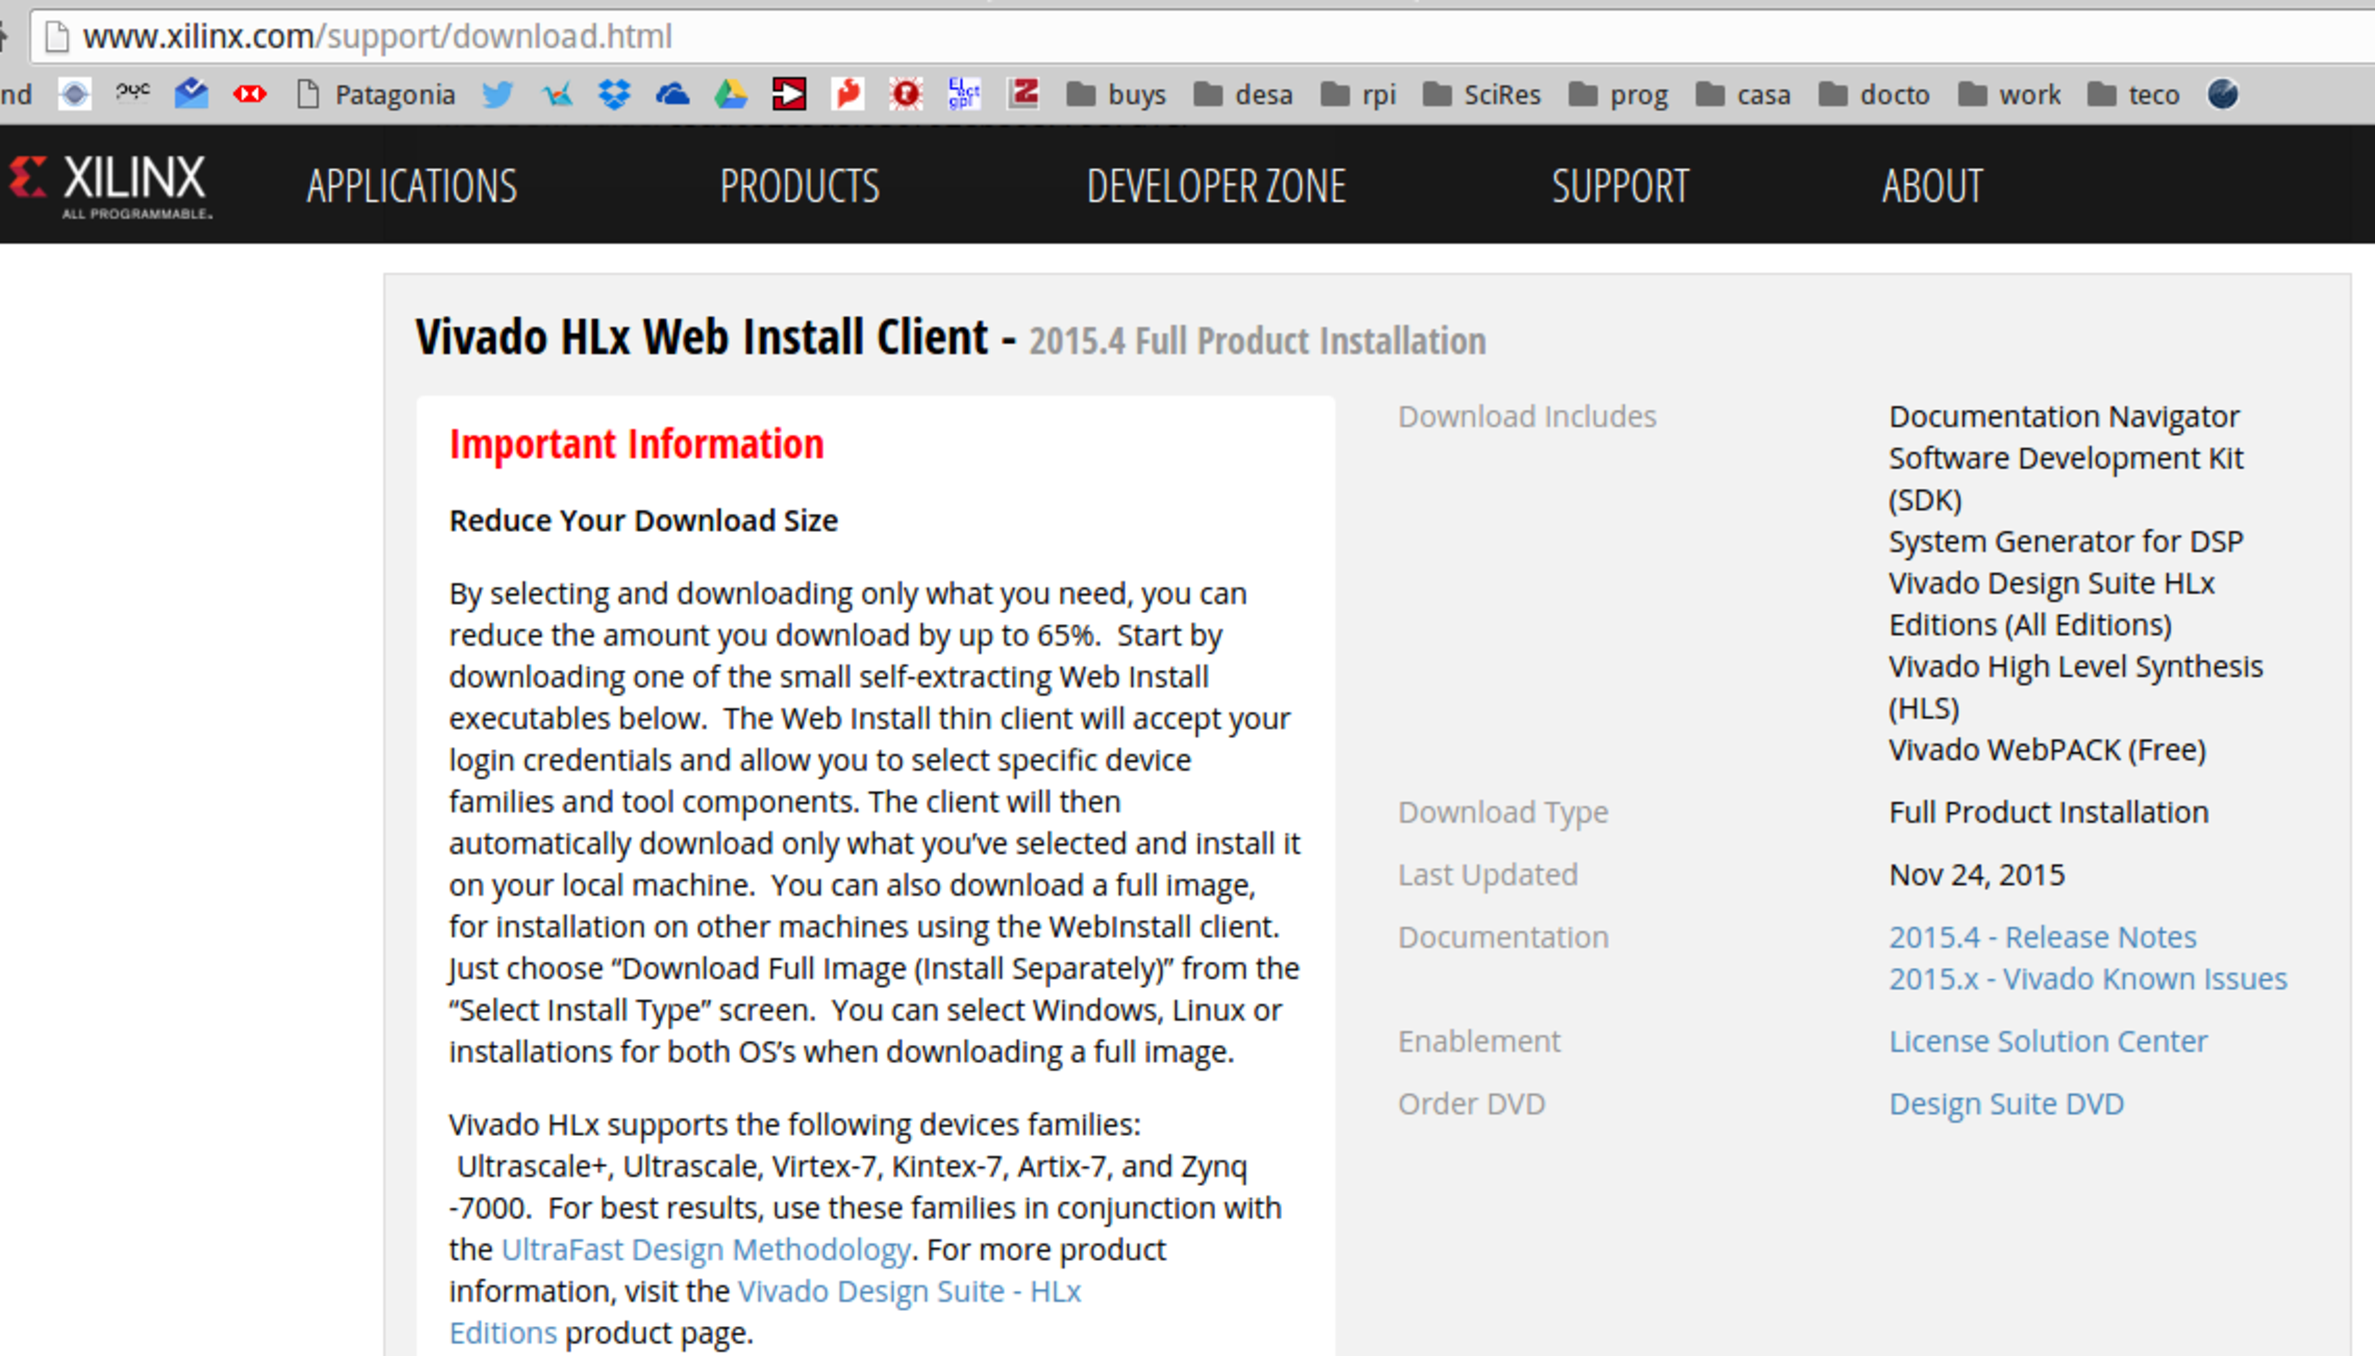
\includegraphics[height=7cm,width=8cm]{vivado_install_client}}
	\caption{XXXXPrimera versión del detector ASCII de $0.25\,m^2$.
	Sirvió como prototipo para demostrar su utilidad.}
	\label{fig:ASCII1} 
\end{figure}

\subsubsection{El cliente web}
  Ejecución
    Para lanzar el cliente una vez descargado:
    \begin{verbatim}
      $ chmod +x Xilinx_Vivado_SDK_2015.4_1118_2_Lin64.bin
      $ sudo ./Xilinx_Vivado_SDK_2015.4_1118_2_Lin64.bin
    \end{verbatim}
    \begin{itemize}
      \item \textbf{Importante: ejecutarlo con permisos de usuario root}
    \end{itemize}
    \begin{center}
    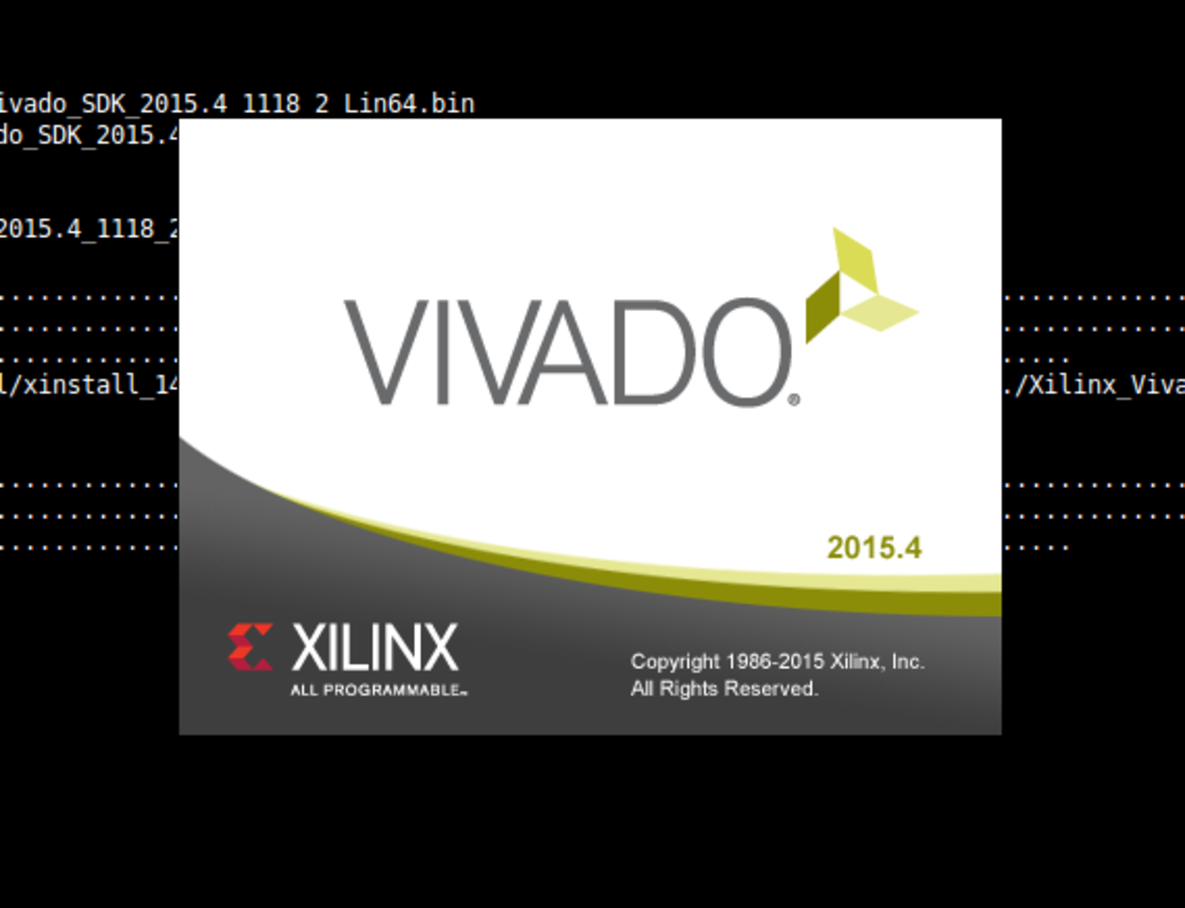
\includegraphics[height=7cm,width=8cm]{vivado_installer_0}
    \end{center}

\subsubsection{Proceso de instalación}
  Utilizar las credenciales de xilinx.com
    En este paso, colocar los datos de registro que hemos generado en
    xilinx.com. En caso de que no hayamos hecho el registro en la página,
    hacerlo ahora.
    \begin{center}
    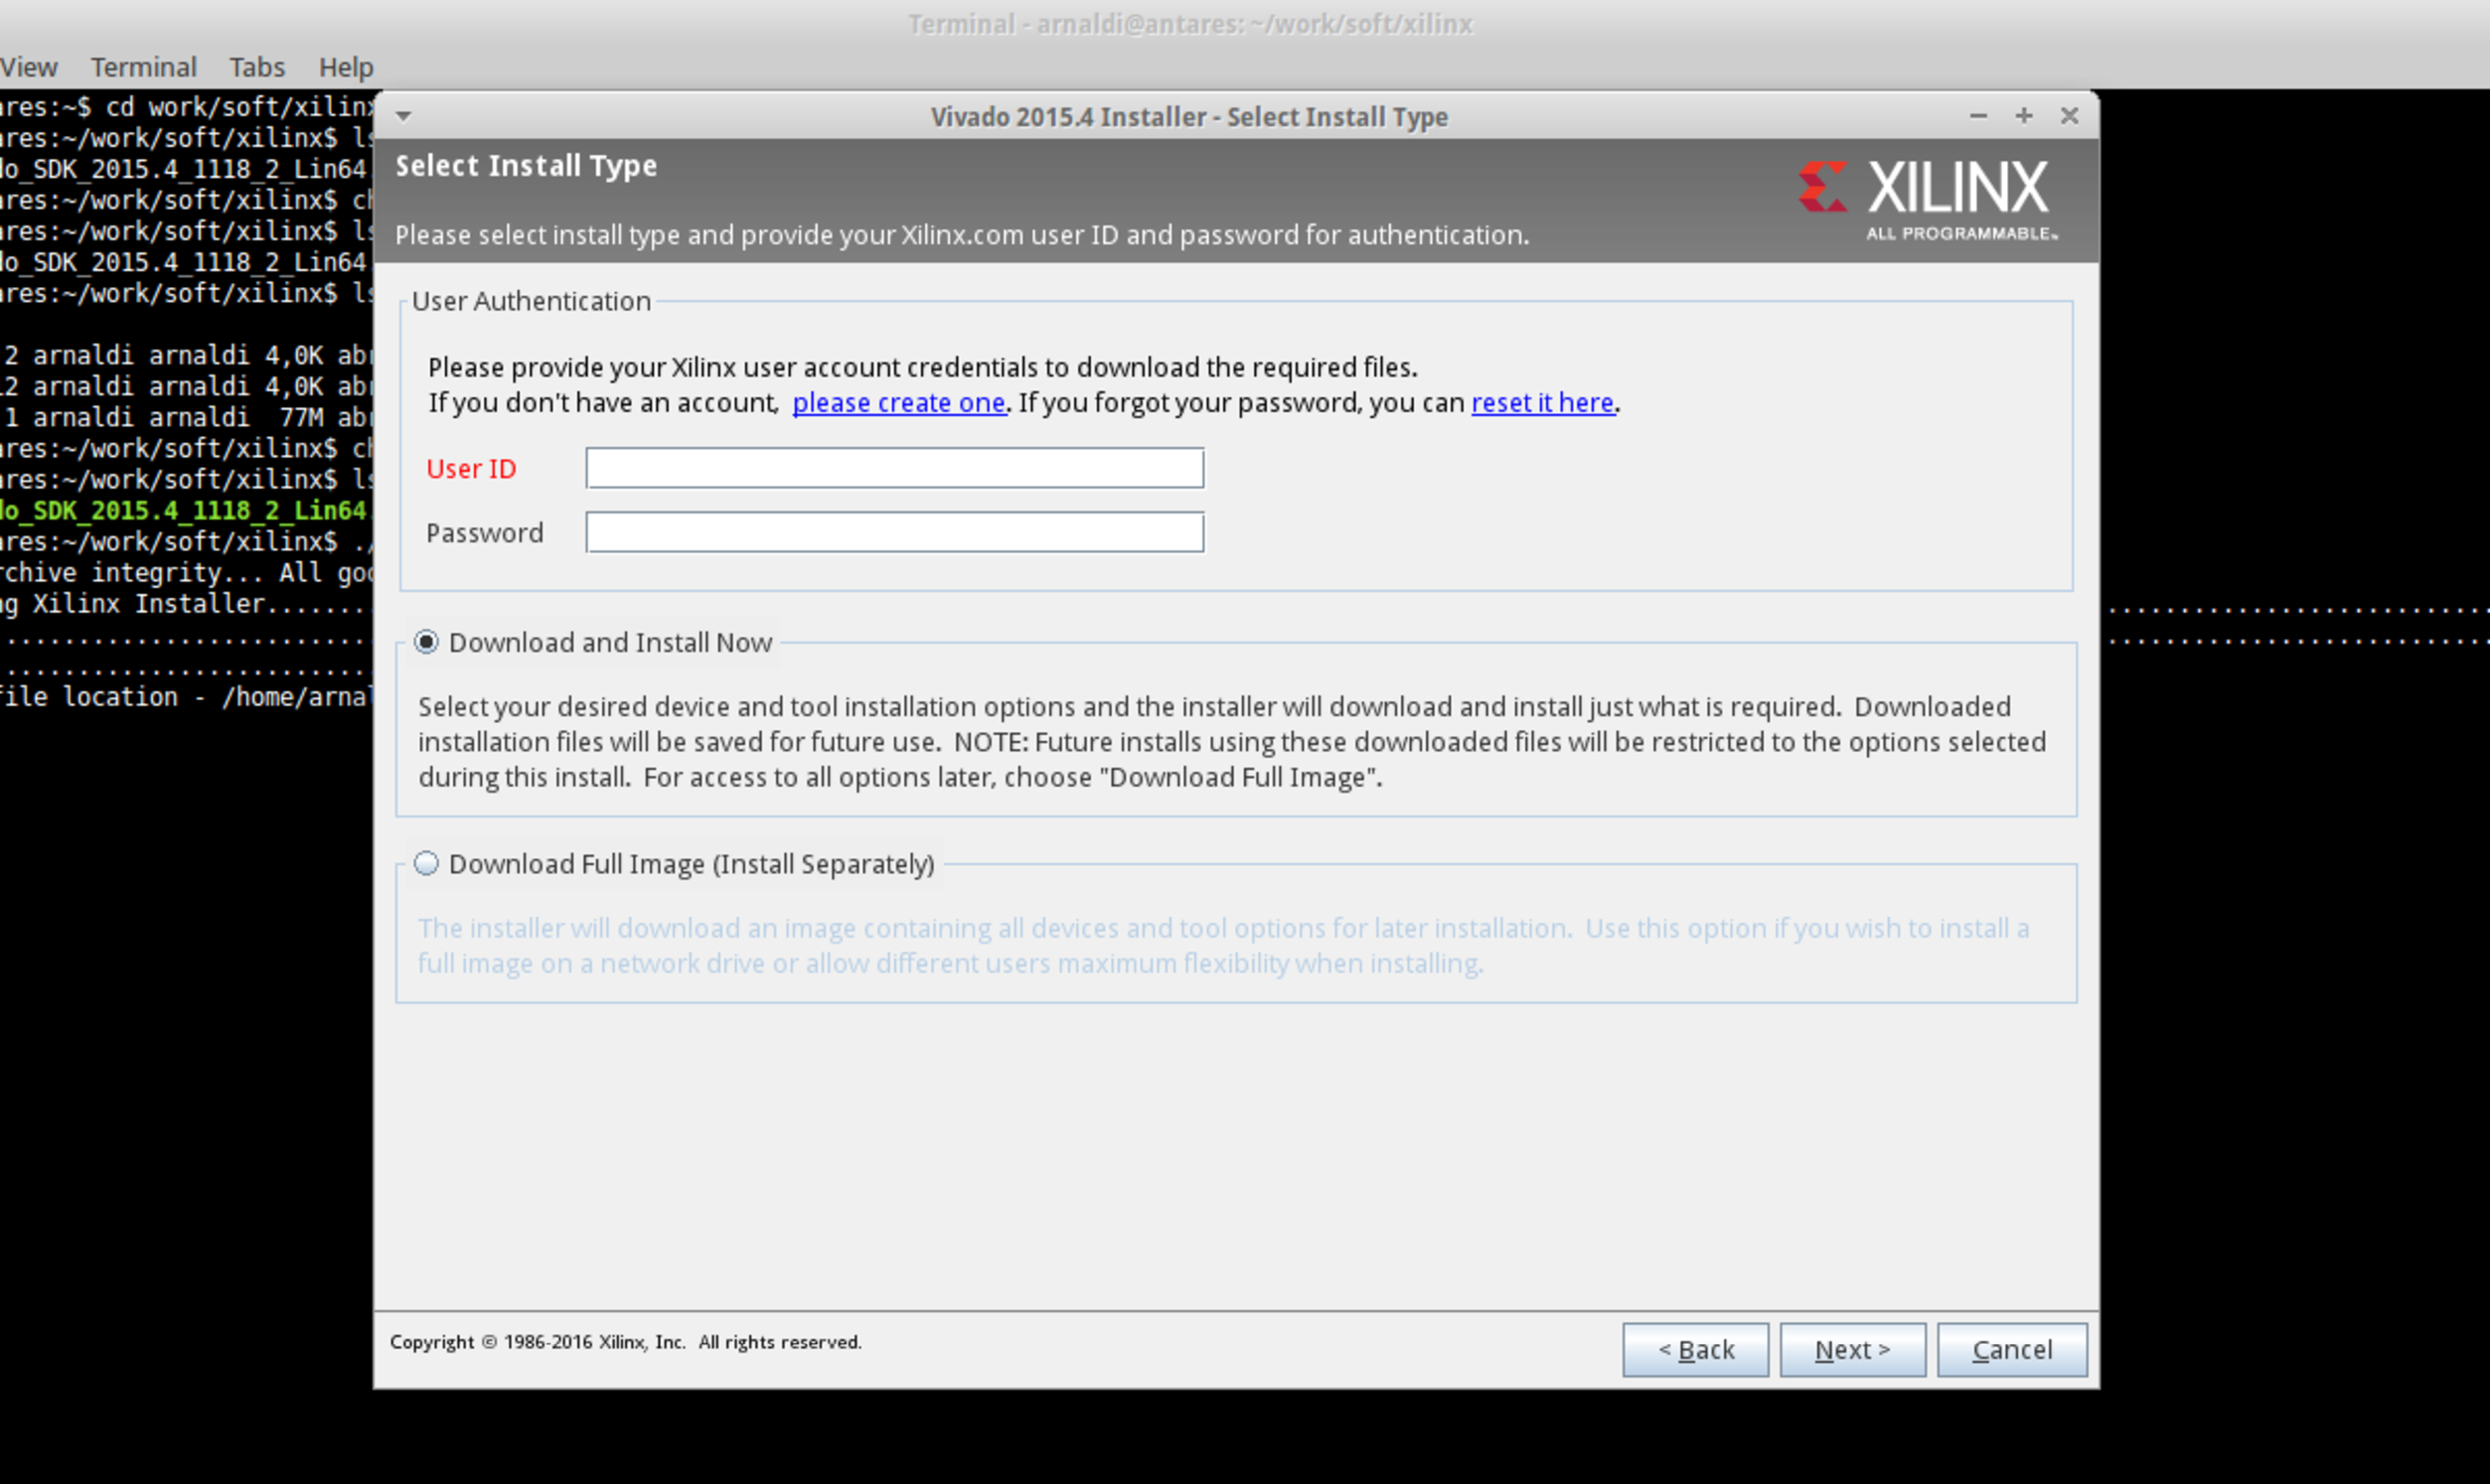
\includegraphics[height=7cm,width=9cm]{vivado_installer_2}
    \end{center}

Elegir Vivado HL Design Edition
    \begin{center}
    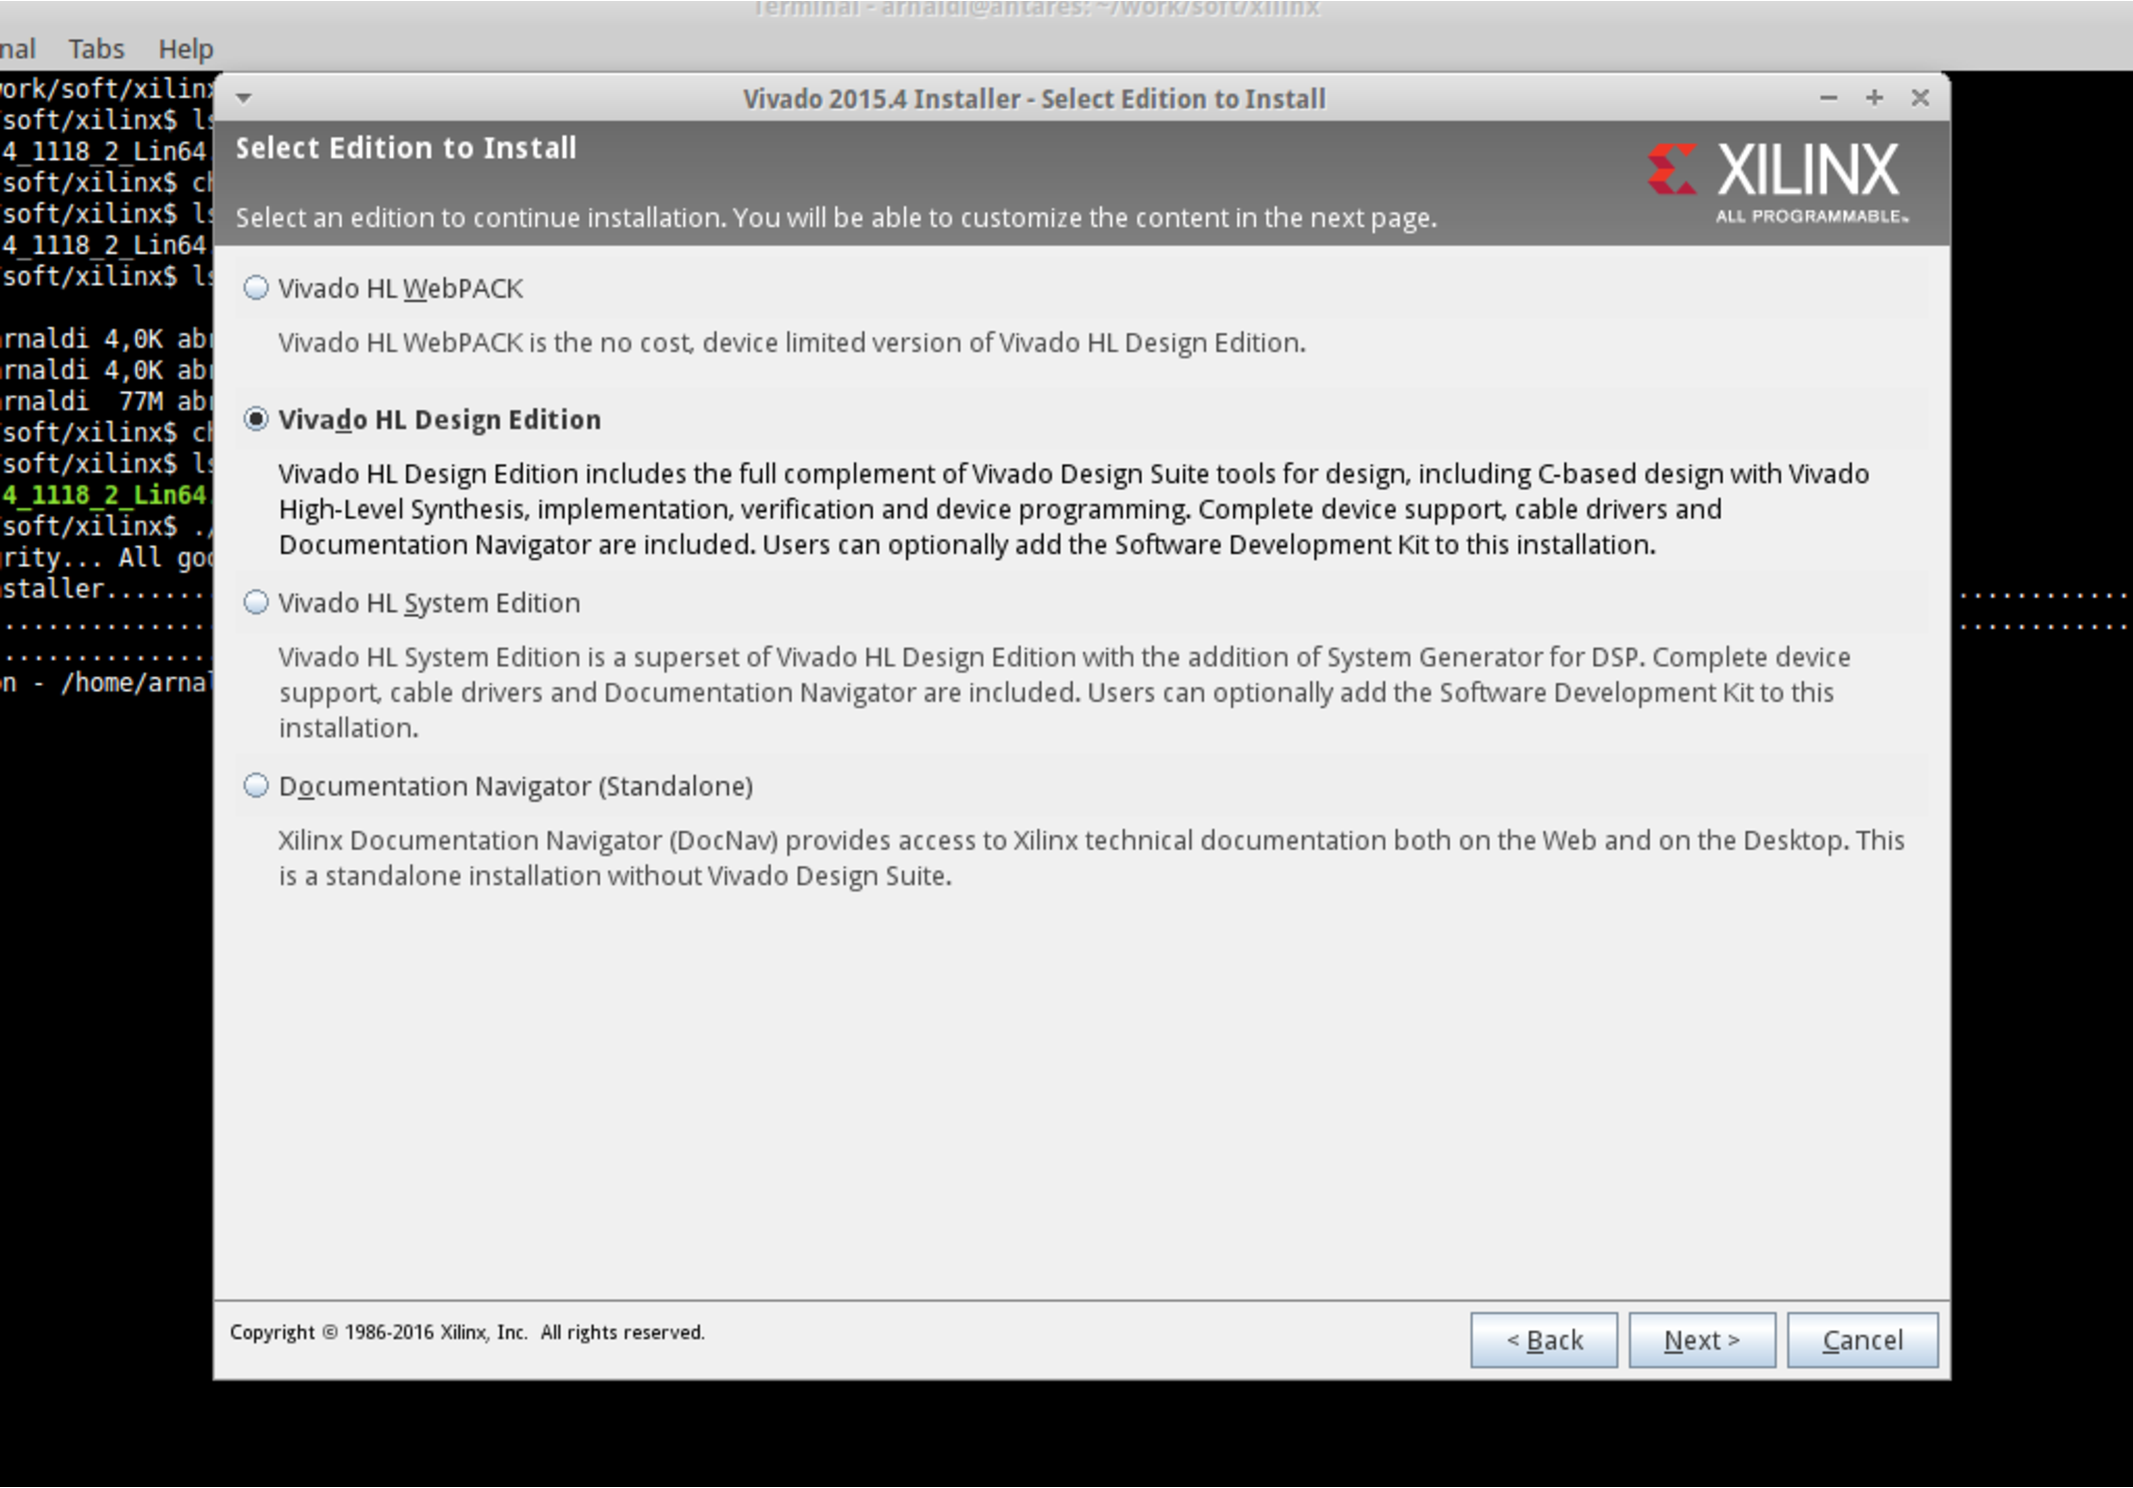
\includegraphics[height=8cm,width=12cm]{vivado_installer_3}
    \end{center}

\subsubsection{Elección de herramientas}
    \begin{itemize}
      \item Se debe tildar la opción \textbf{Software Development Kit} (SDK)
dentro de la solapa Design Tools.
      \item En la solapa Devices, destildar las opciones \textbf{UltraScale} y
            \textbf{UltraScale+}.
    \end{itemize}
    \begin{center}
    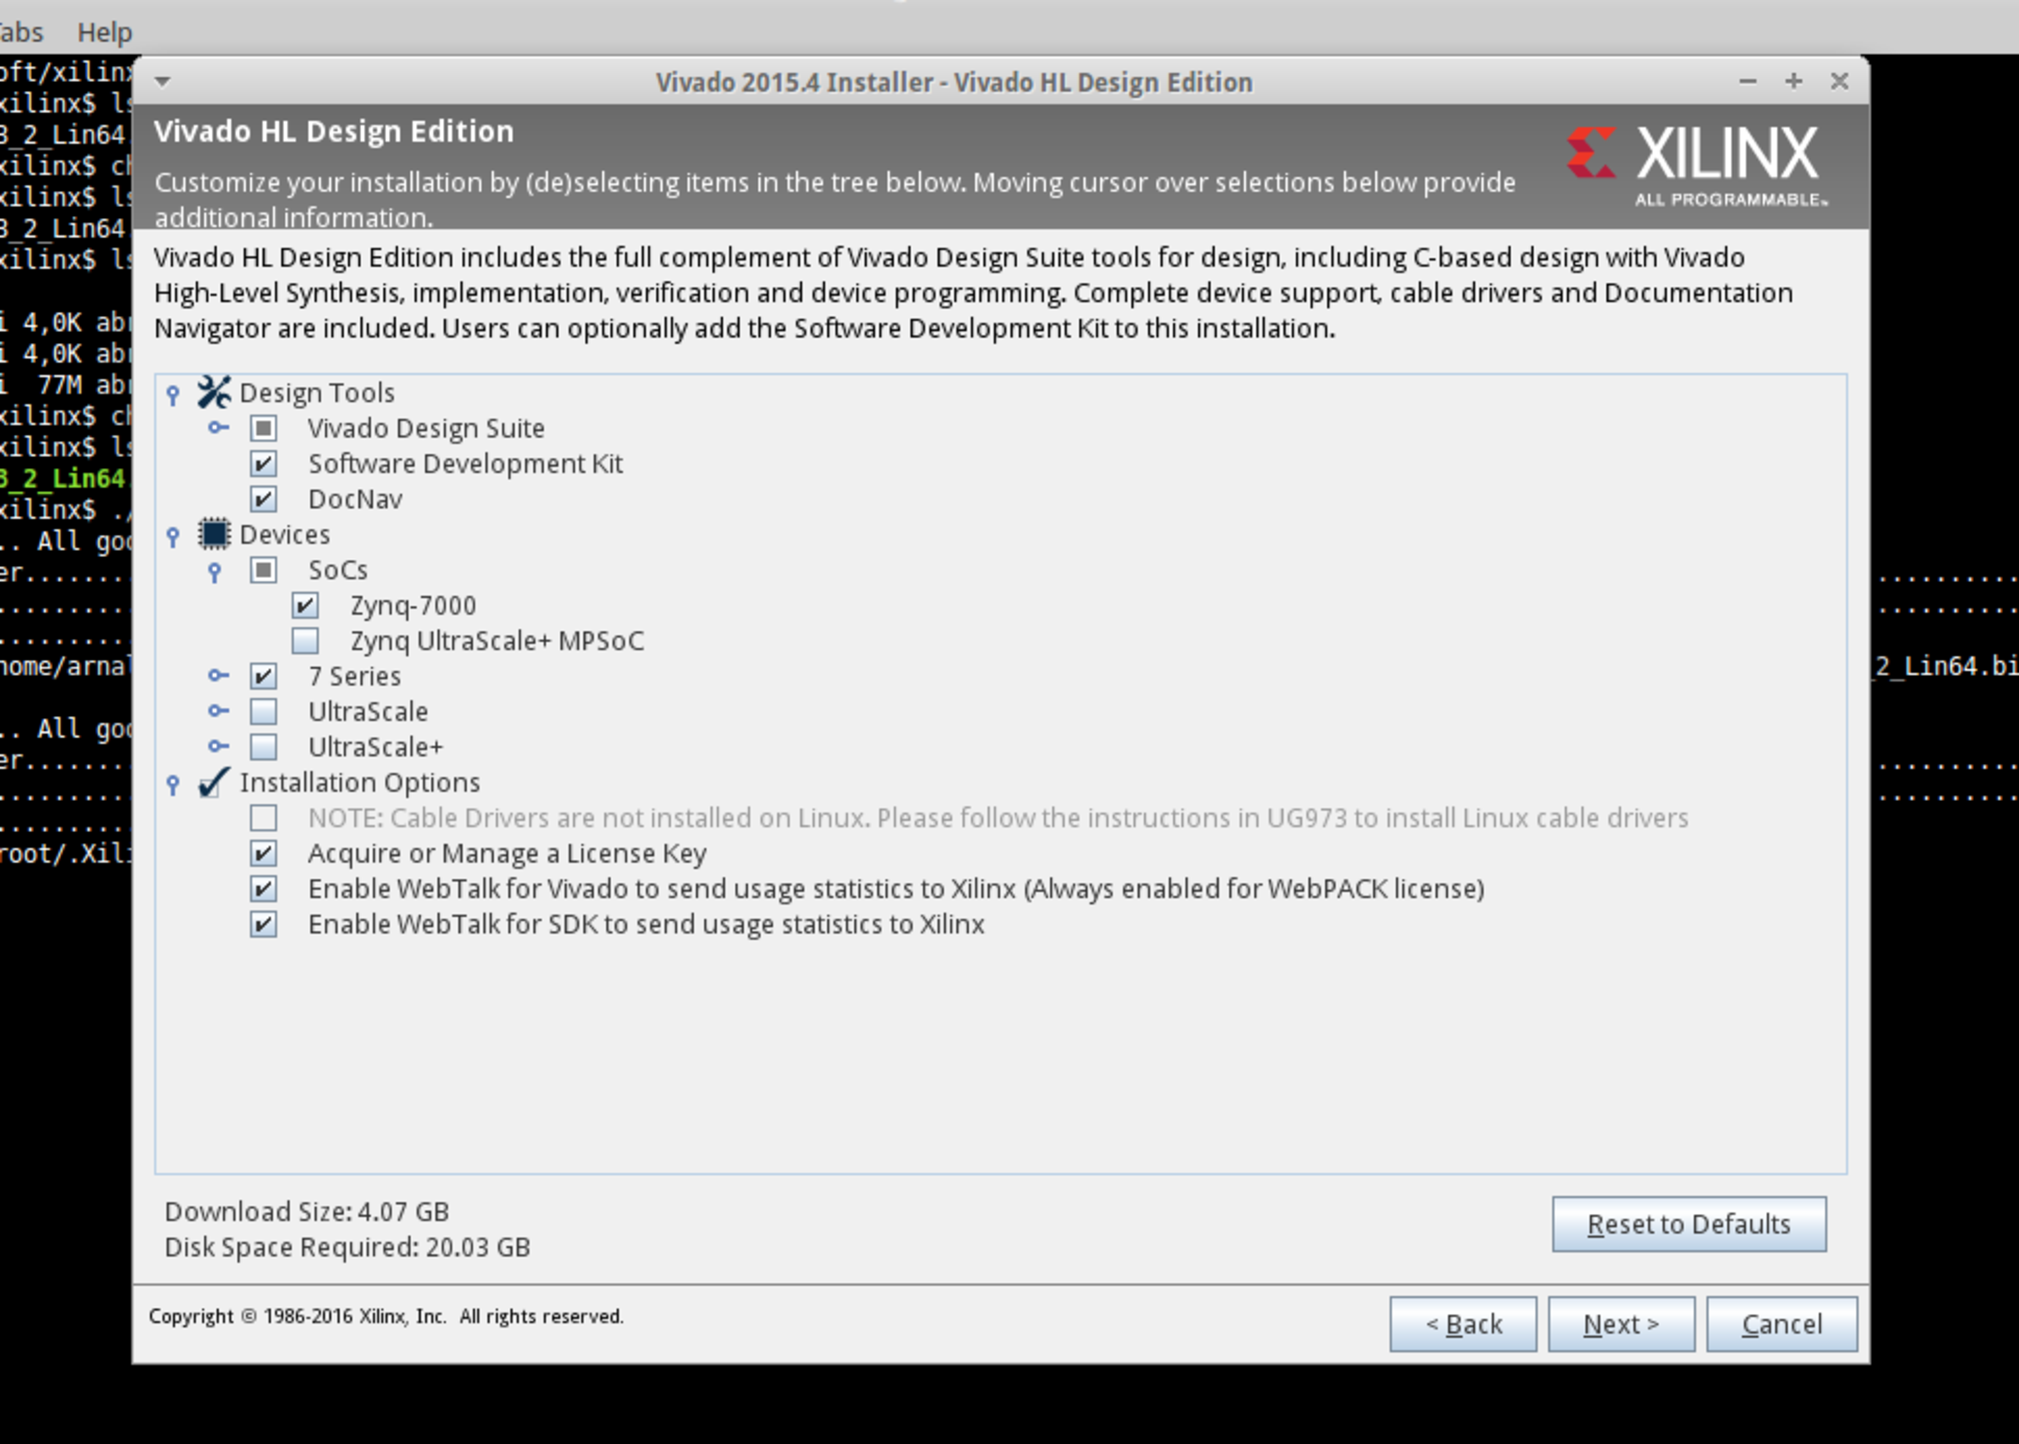
\includegraphics[height=7cm,width=9cm]{vivado_installer_4}
    \end{center}

    \begin{center}
    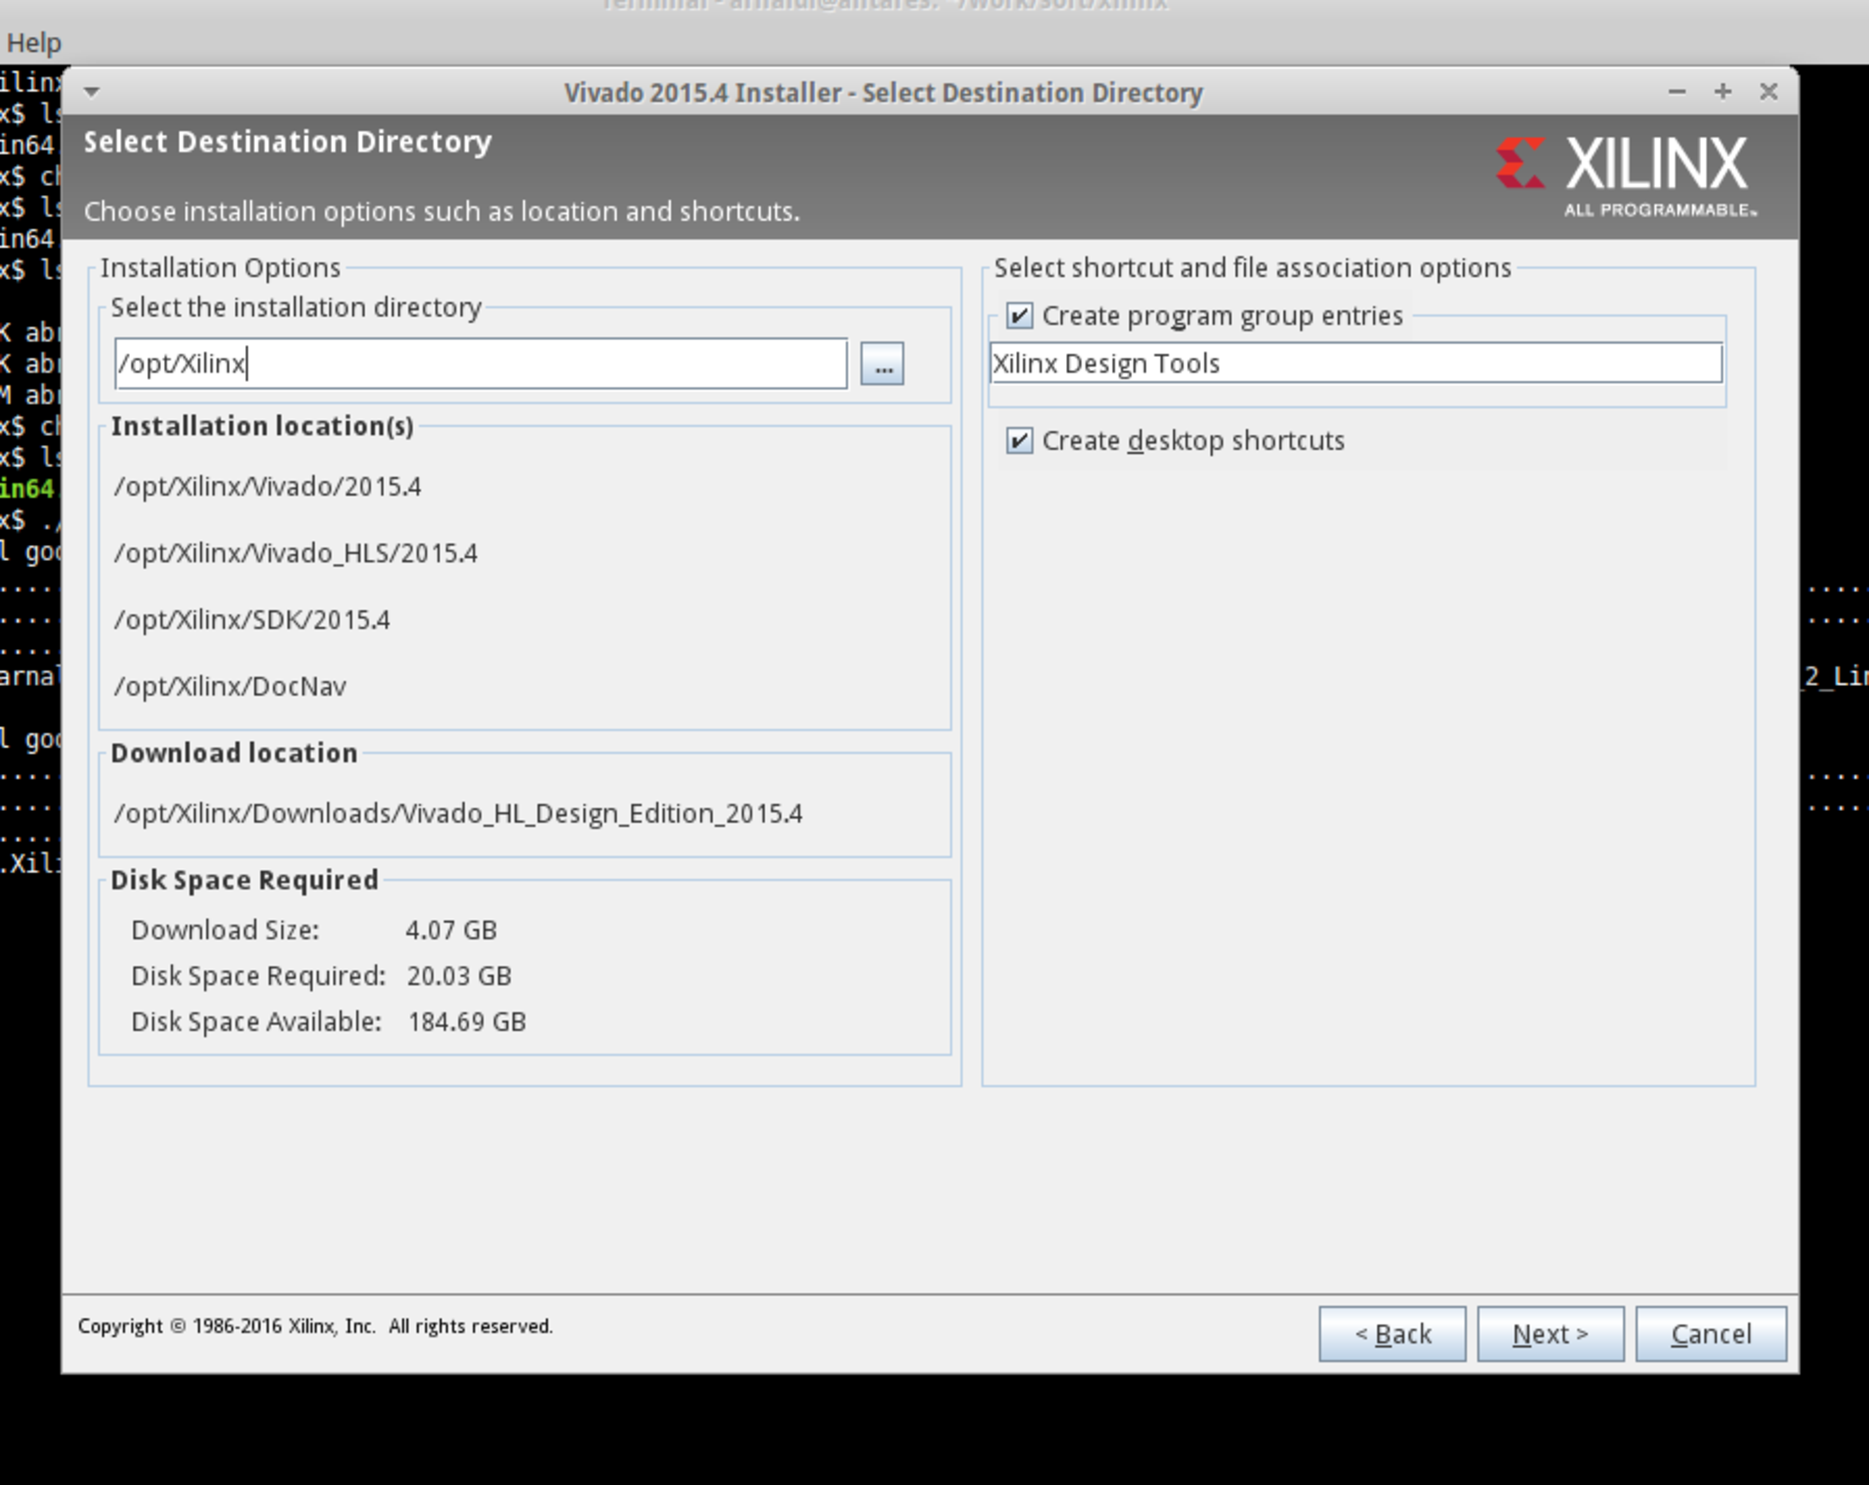
\includegraphics[height=8cm,width=12cm]{vivado_installer_5}
    \end{center}

    \begin{center}
    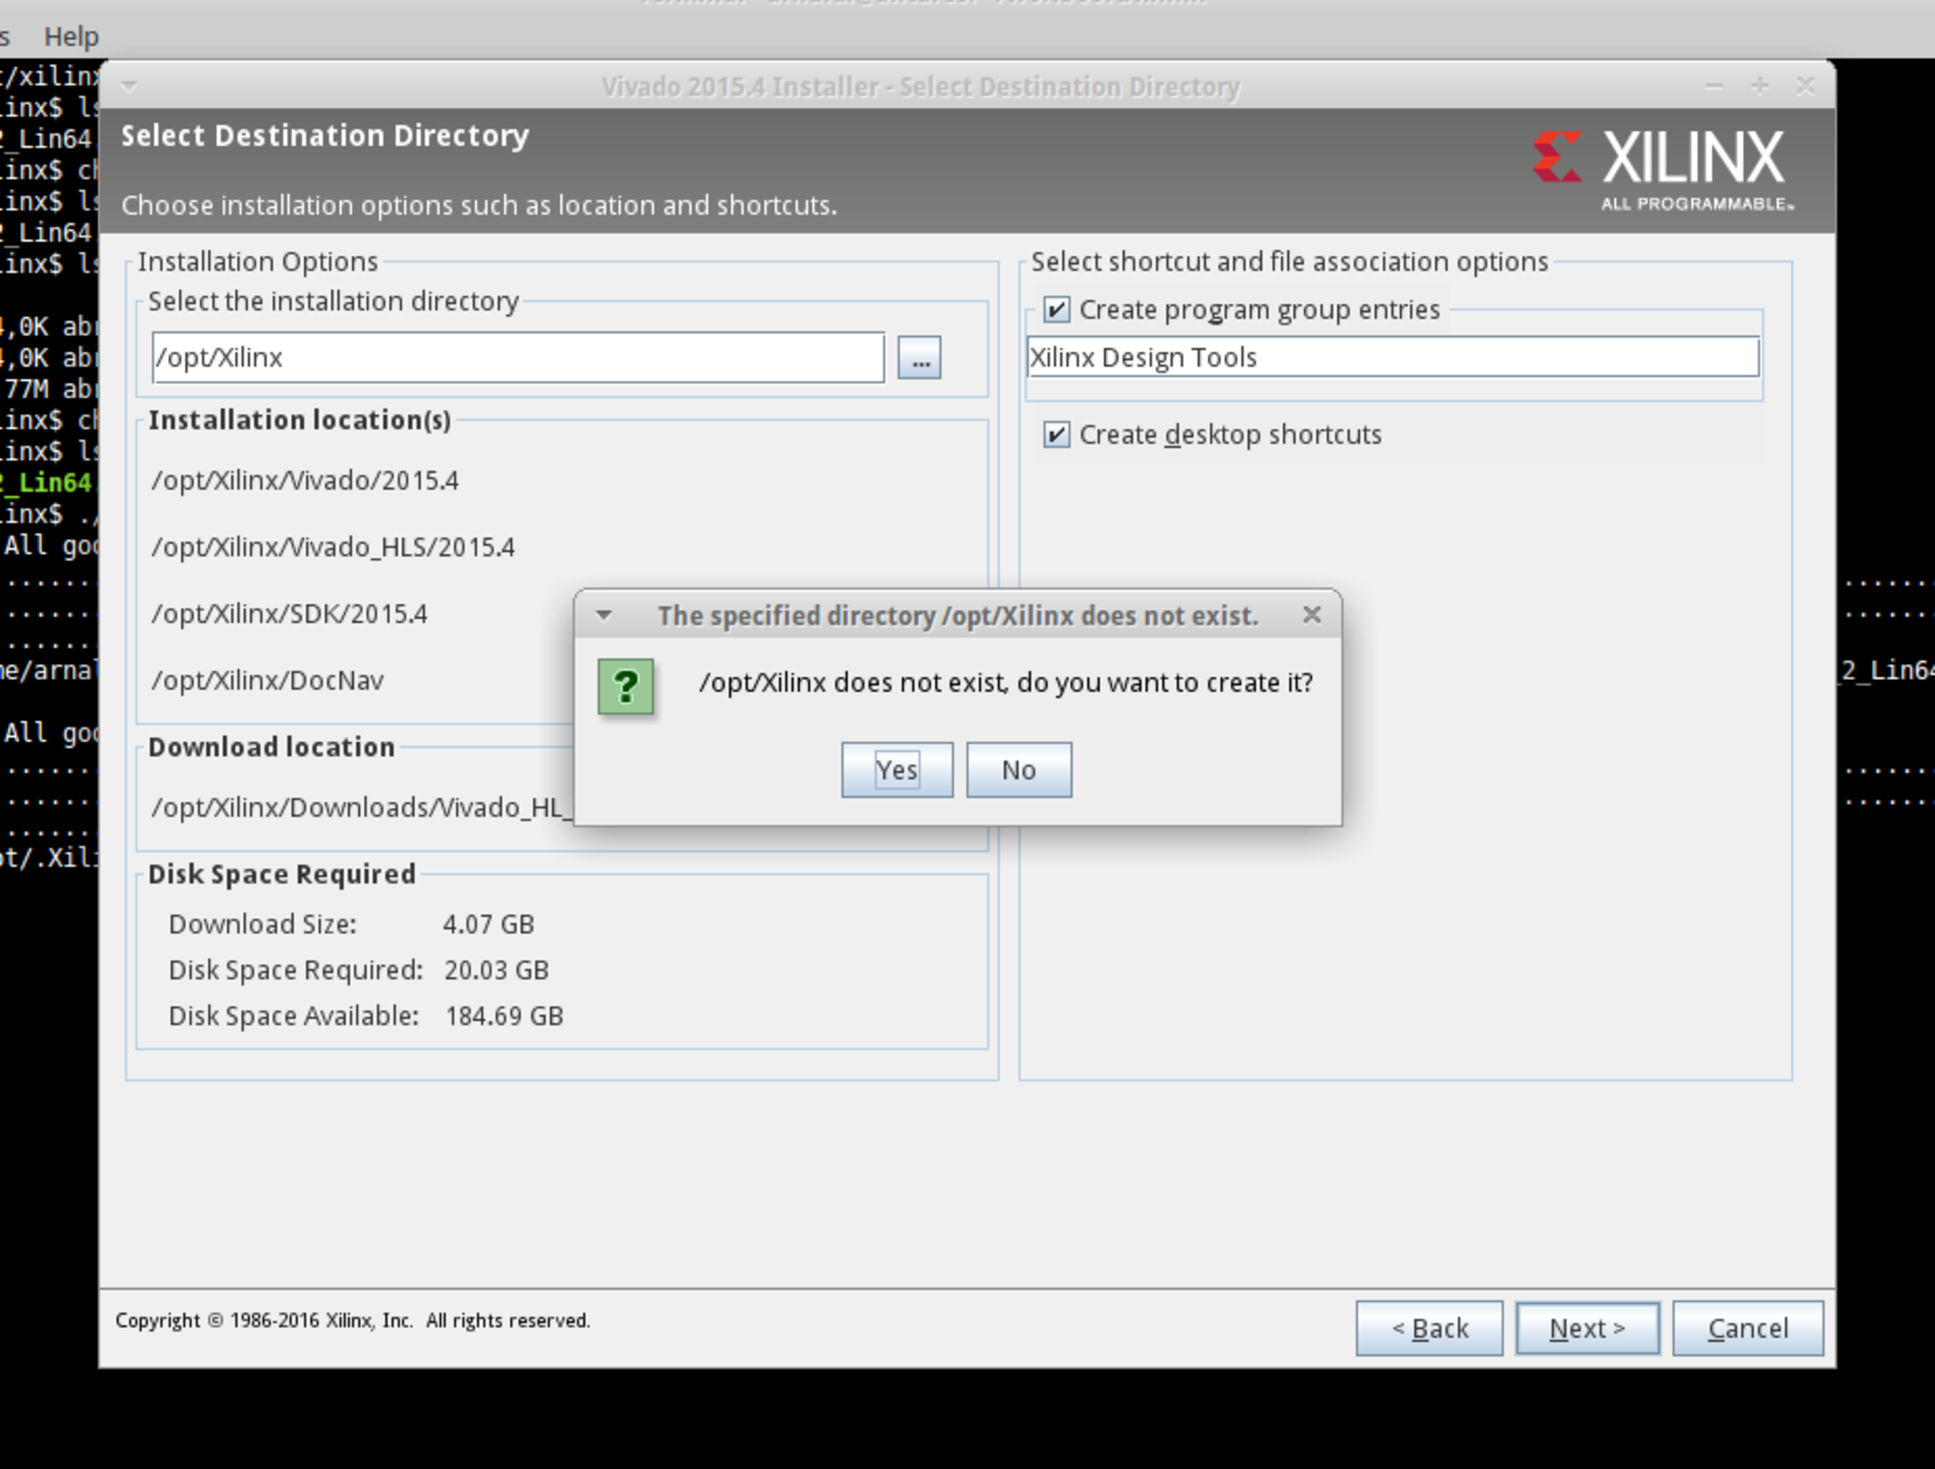
\includegraphics[height=8cm,width=12cm]{vivado_installer_6}
    \end{center}

    \begin{center}
    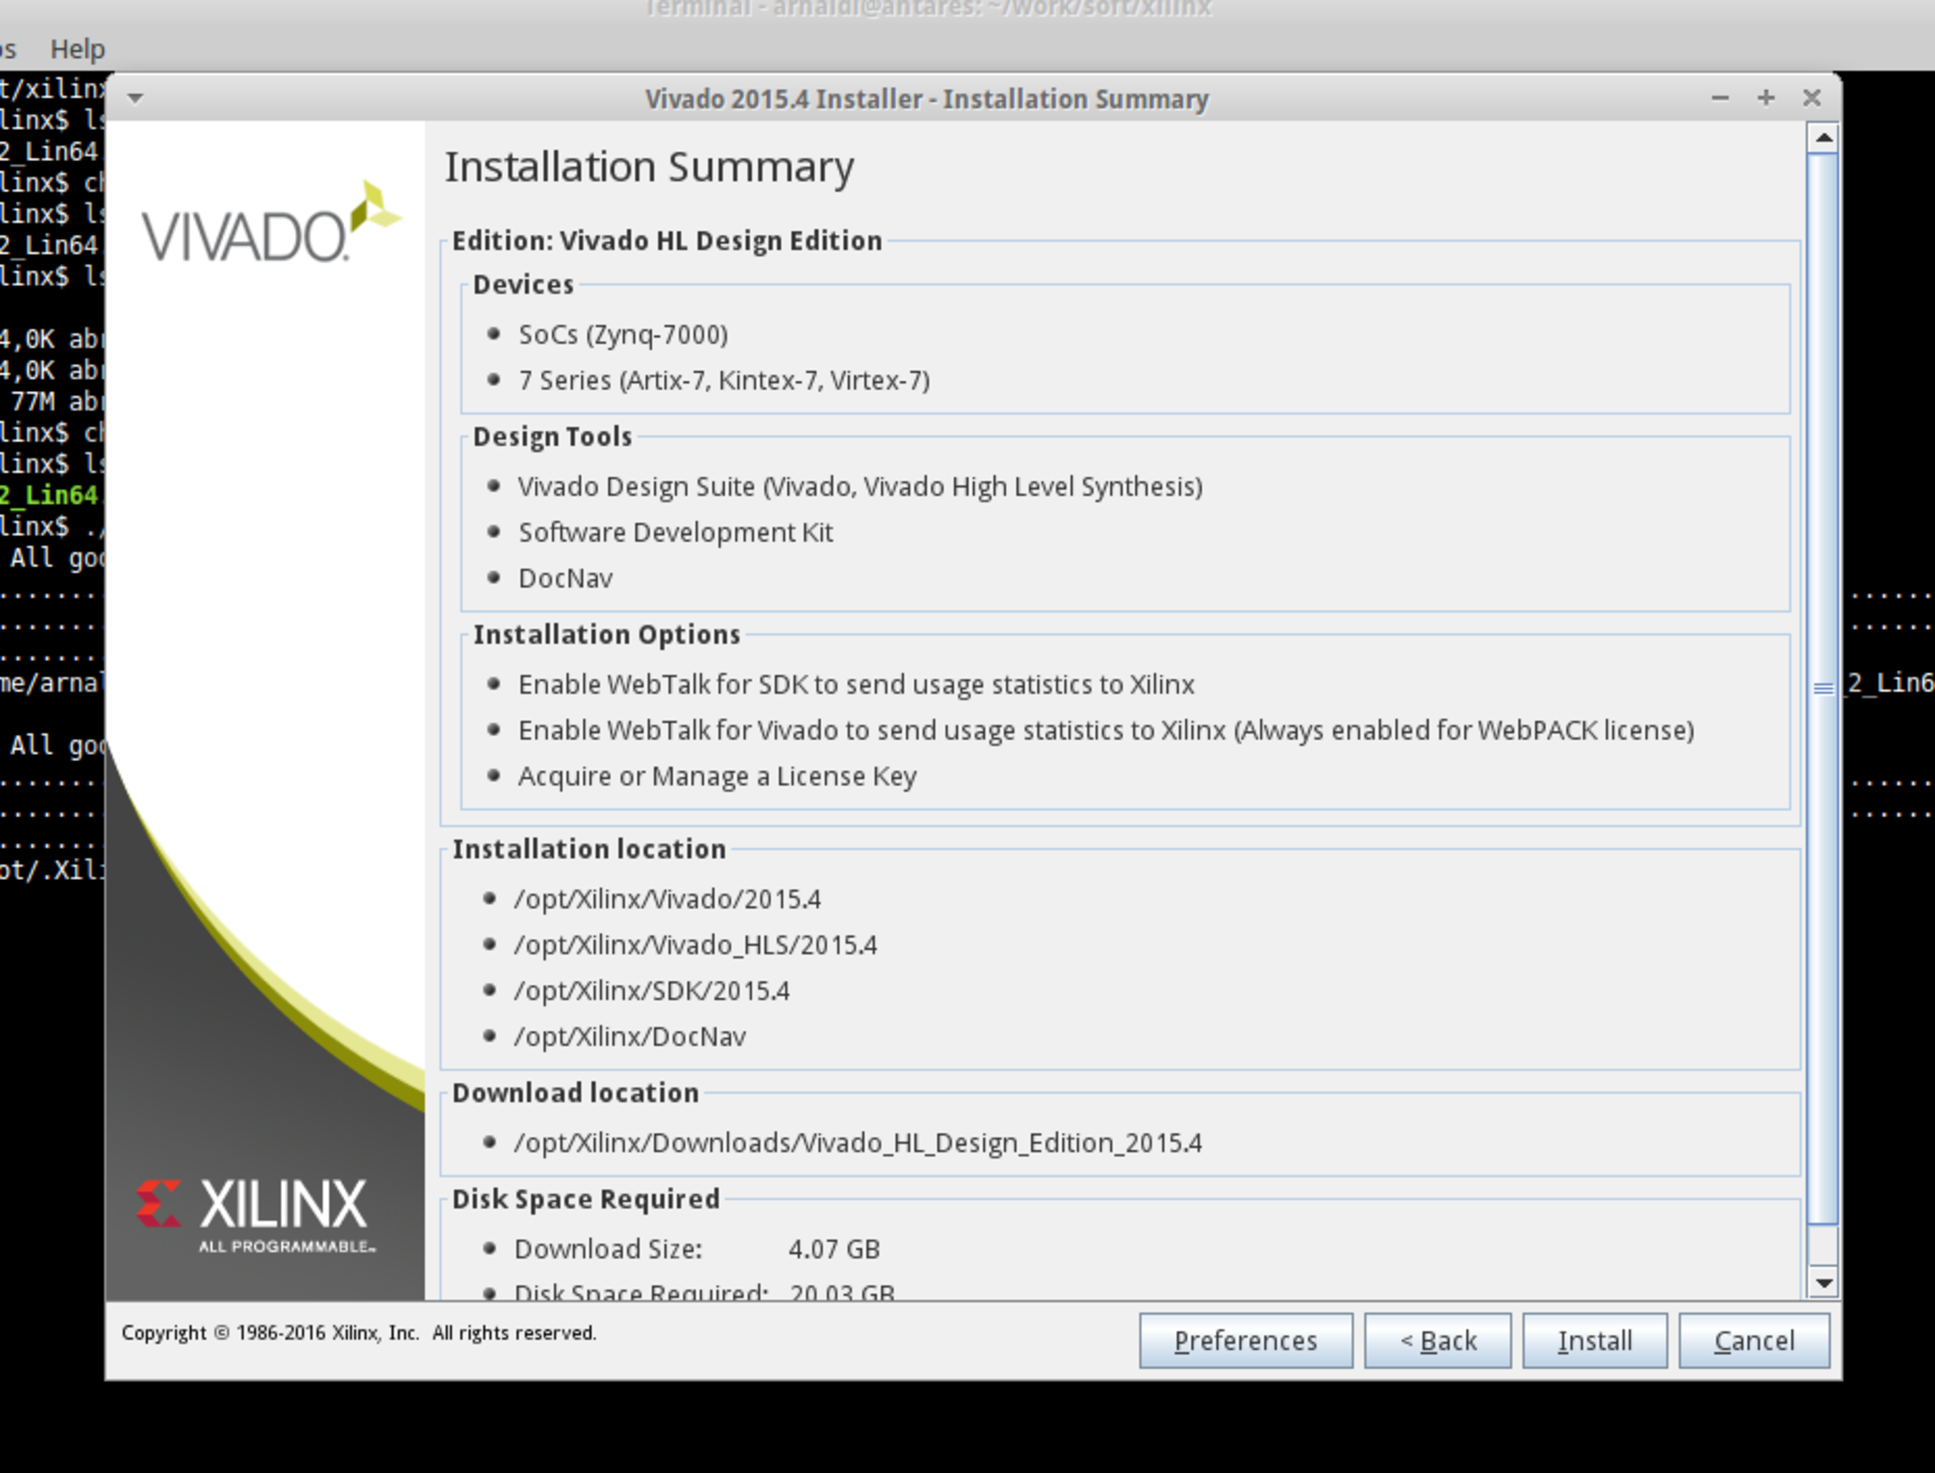
\includegraphics[height=8cm,width=12cm]{vivado_installer_7}
    \end{center}

    \begin{center}
    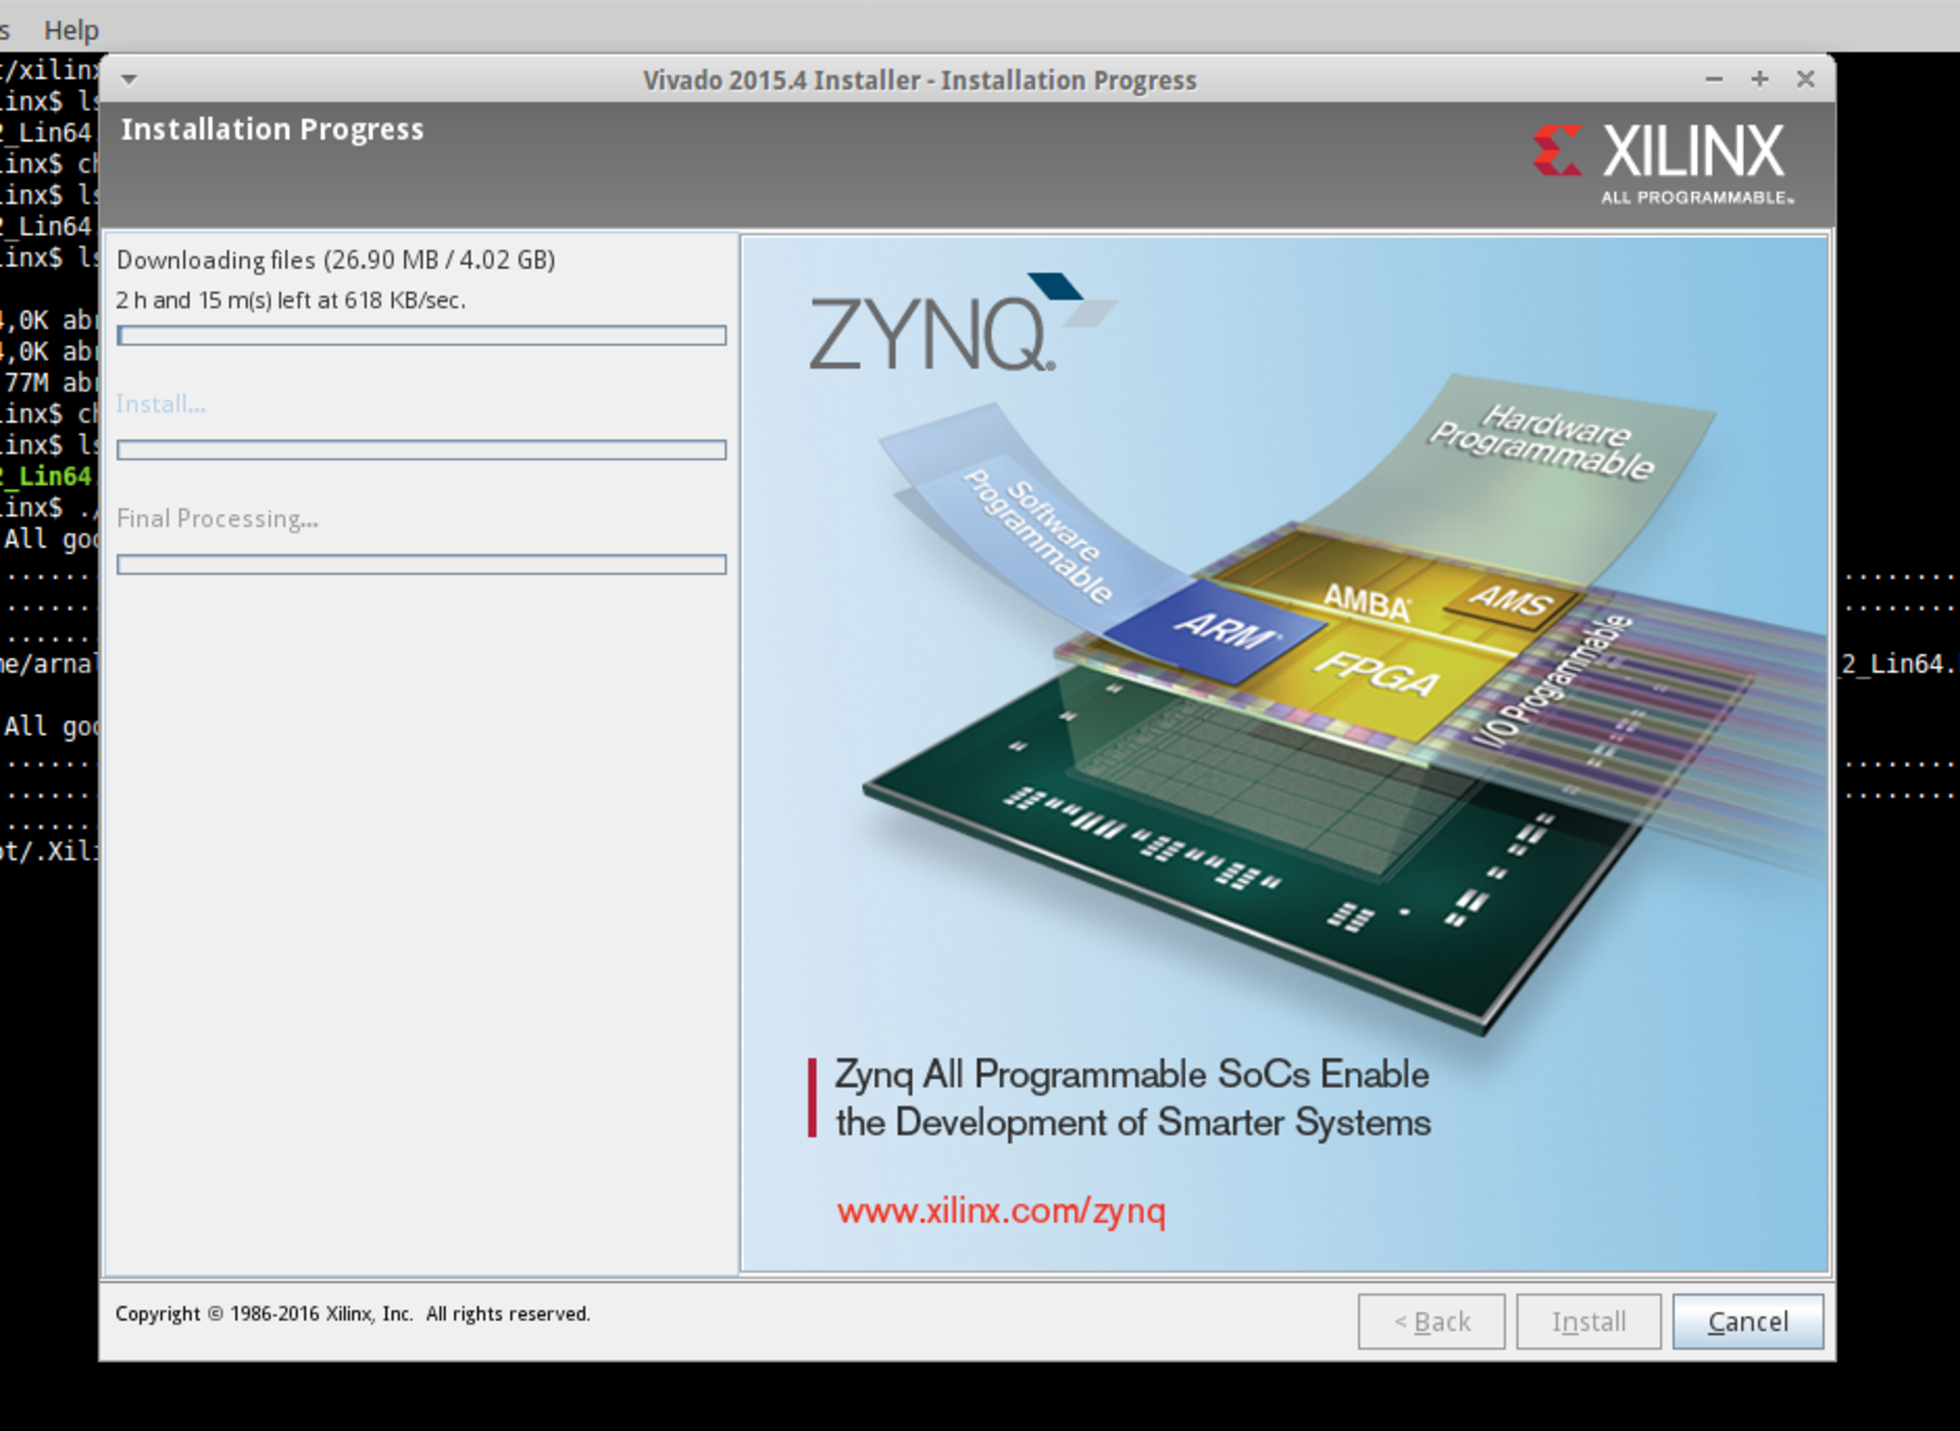
\includegraphics[height=8cm,width=12cm]{vivado_installer_8}
    \end{center}

    \begin{center}
    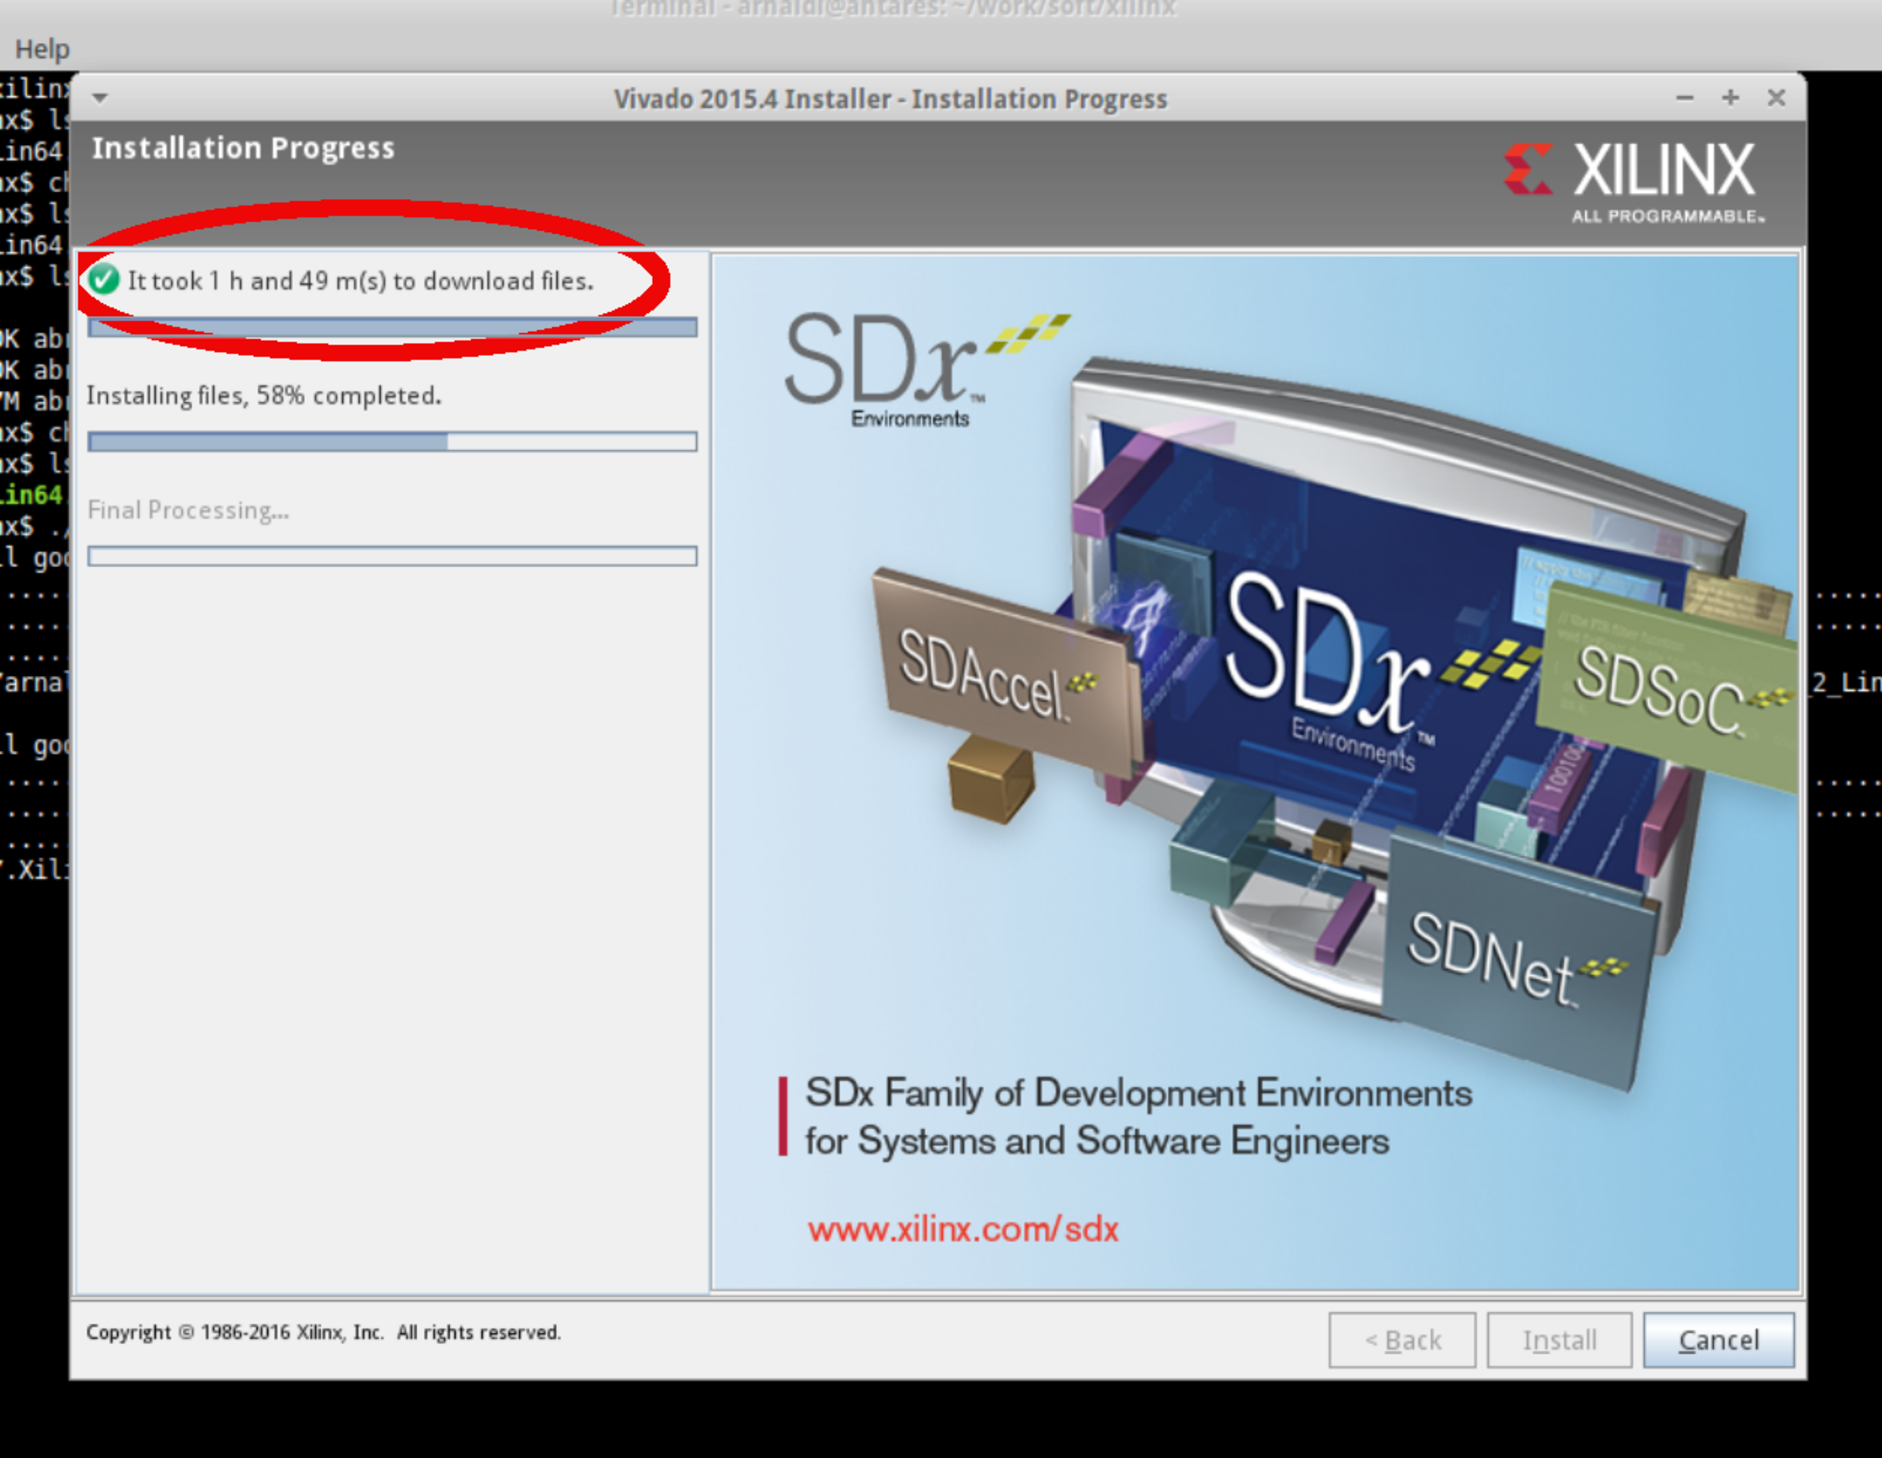
\includegraphics[height=8cm,width=12cm]{vivado_installer_9}
    \end{center}

\subsubsection{Licenciamiento}

    \begin{center}
    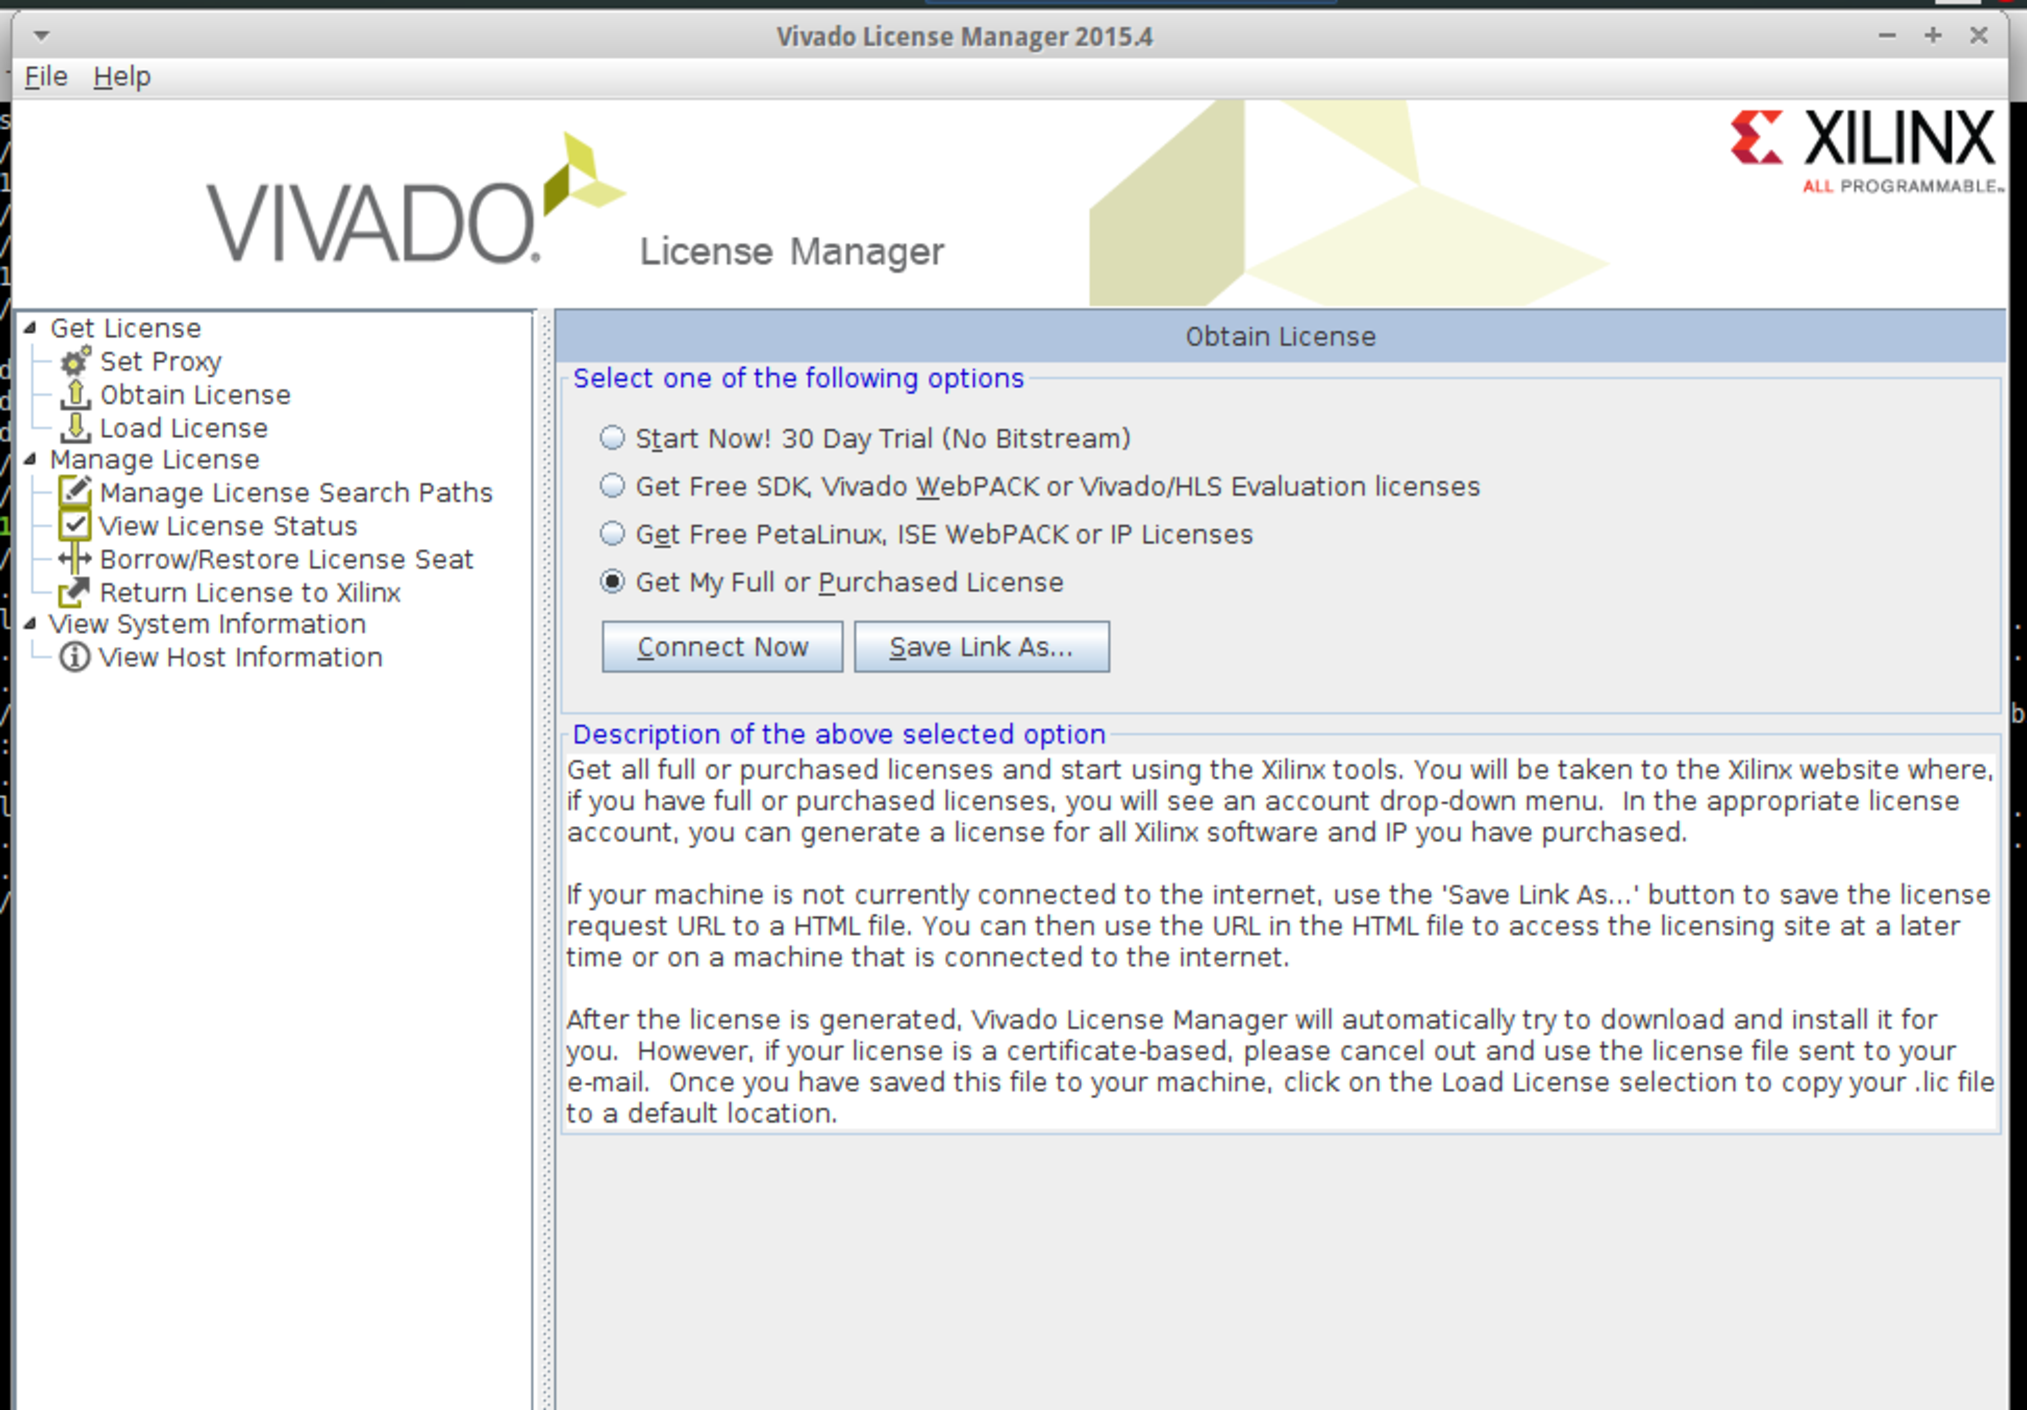
\includegraphics[height=8cm,width=12cm]{vivado_installer_10}
    \end{center}

    \begin{center}
    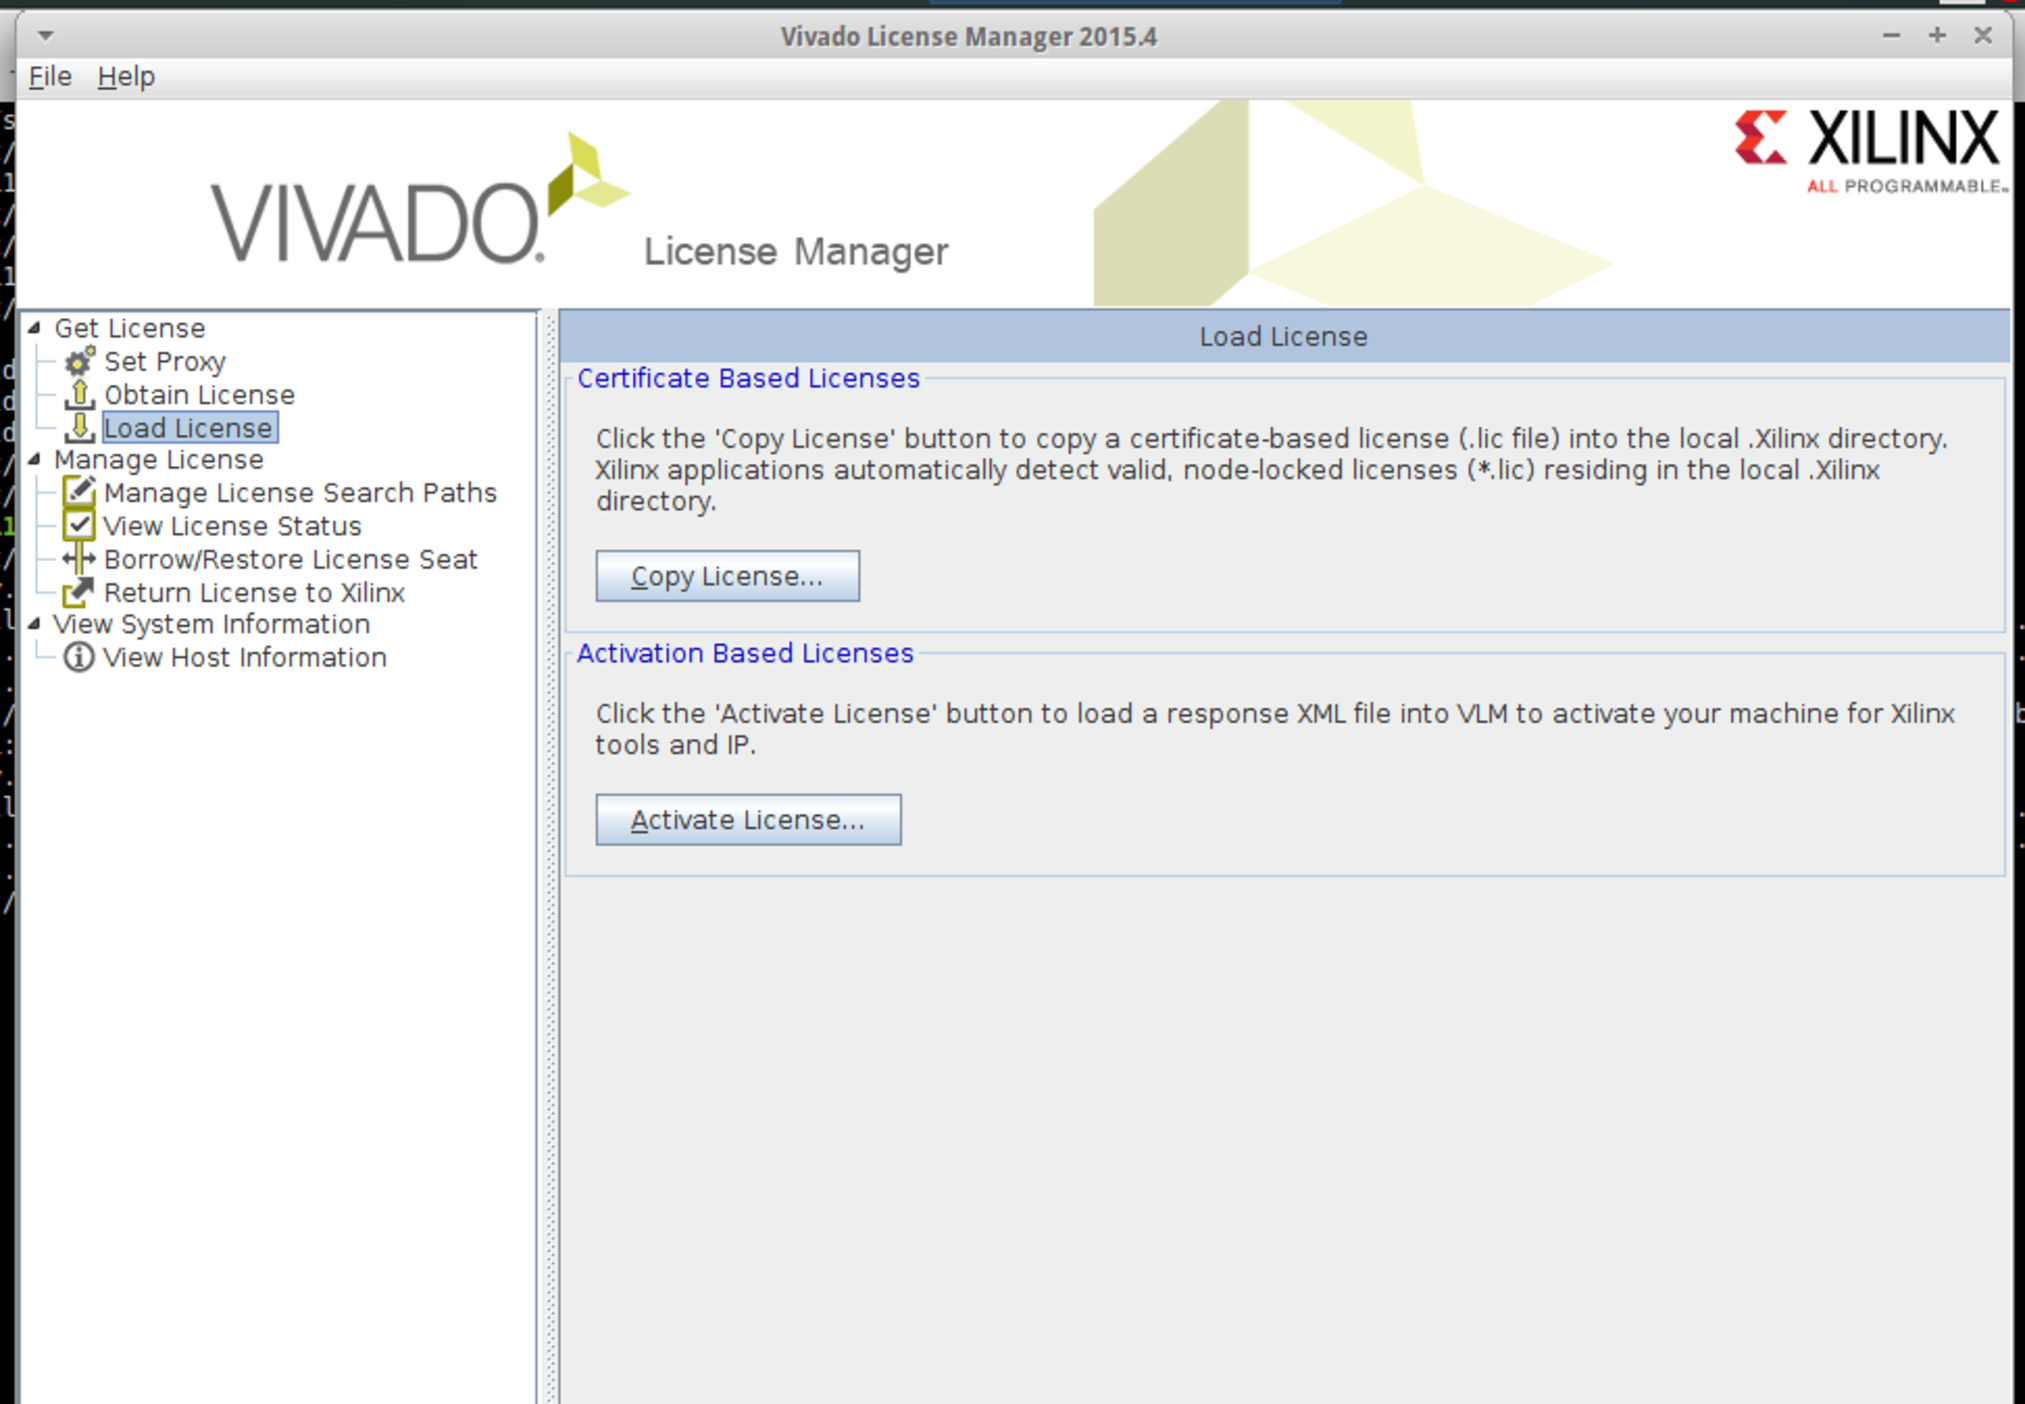
\includegraphics[height=8cm,width=12cm]{vivado_installer_11}
    \end{center}

    \begin{center}
    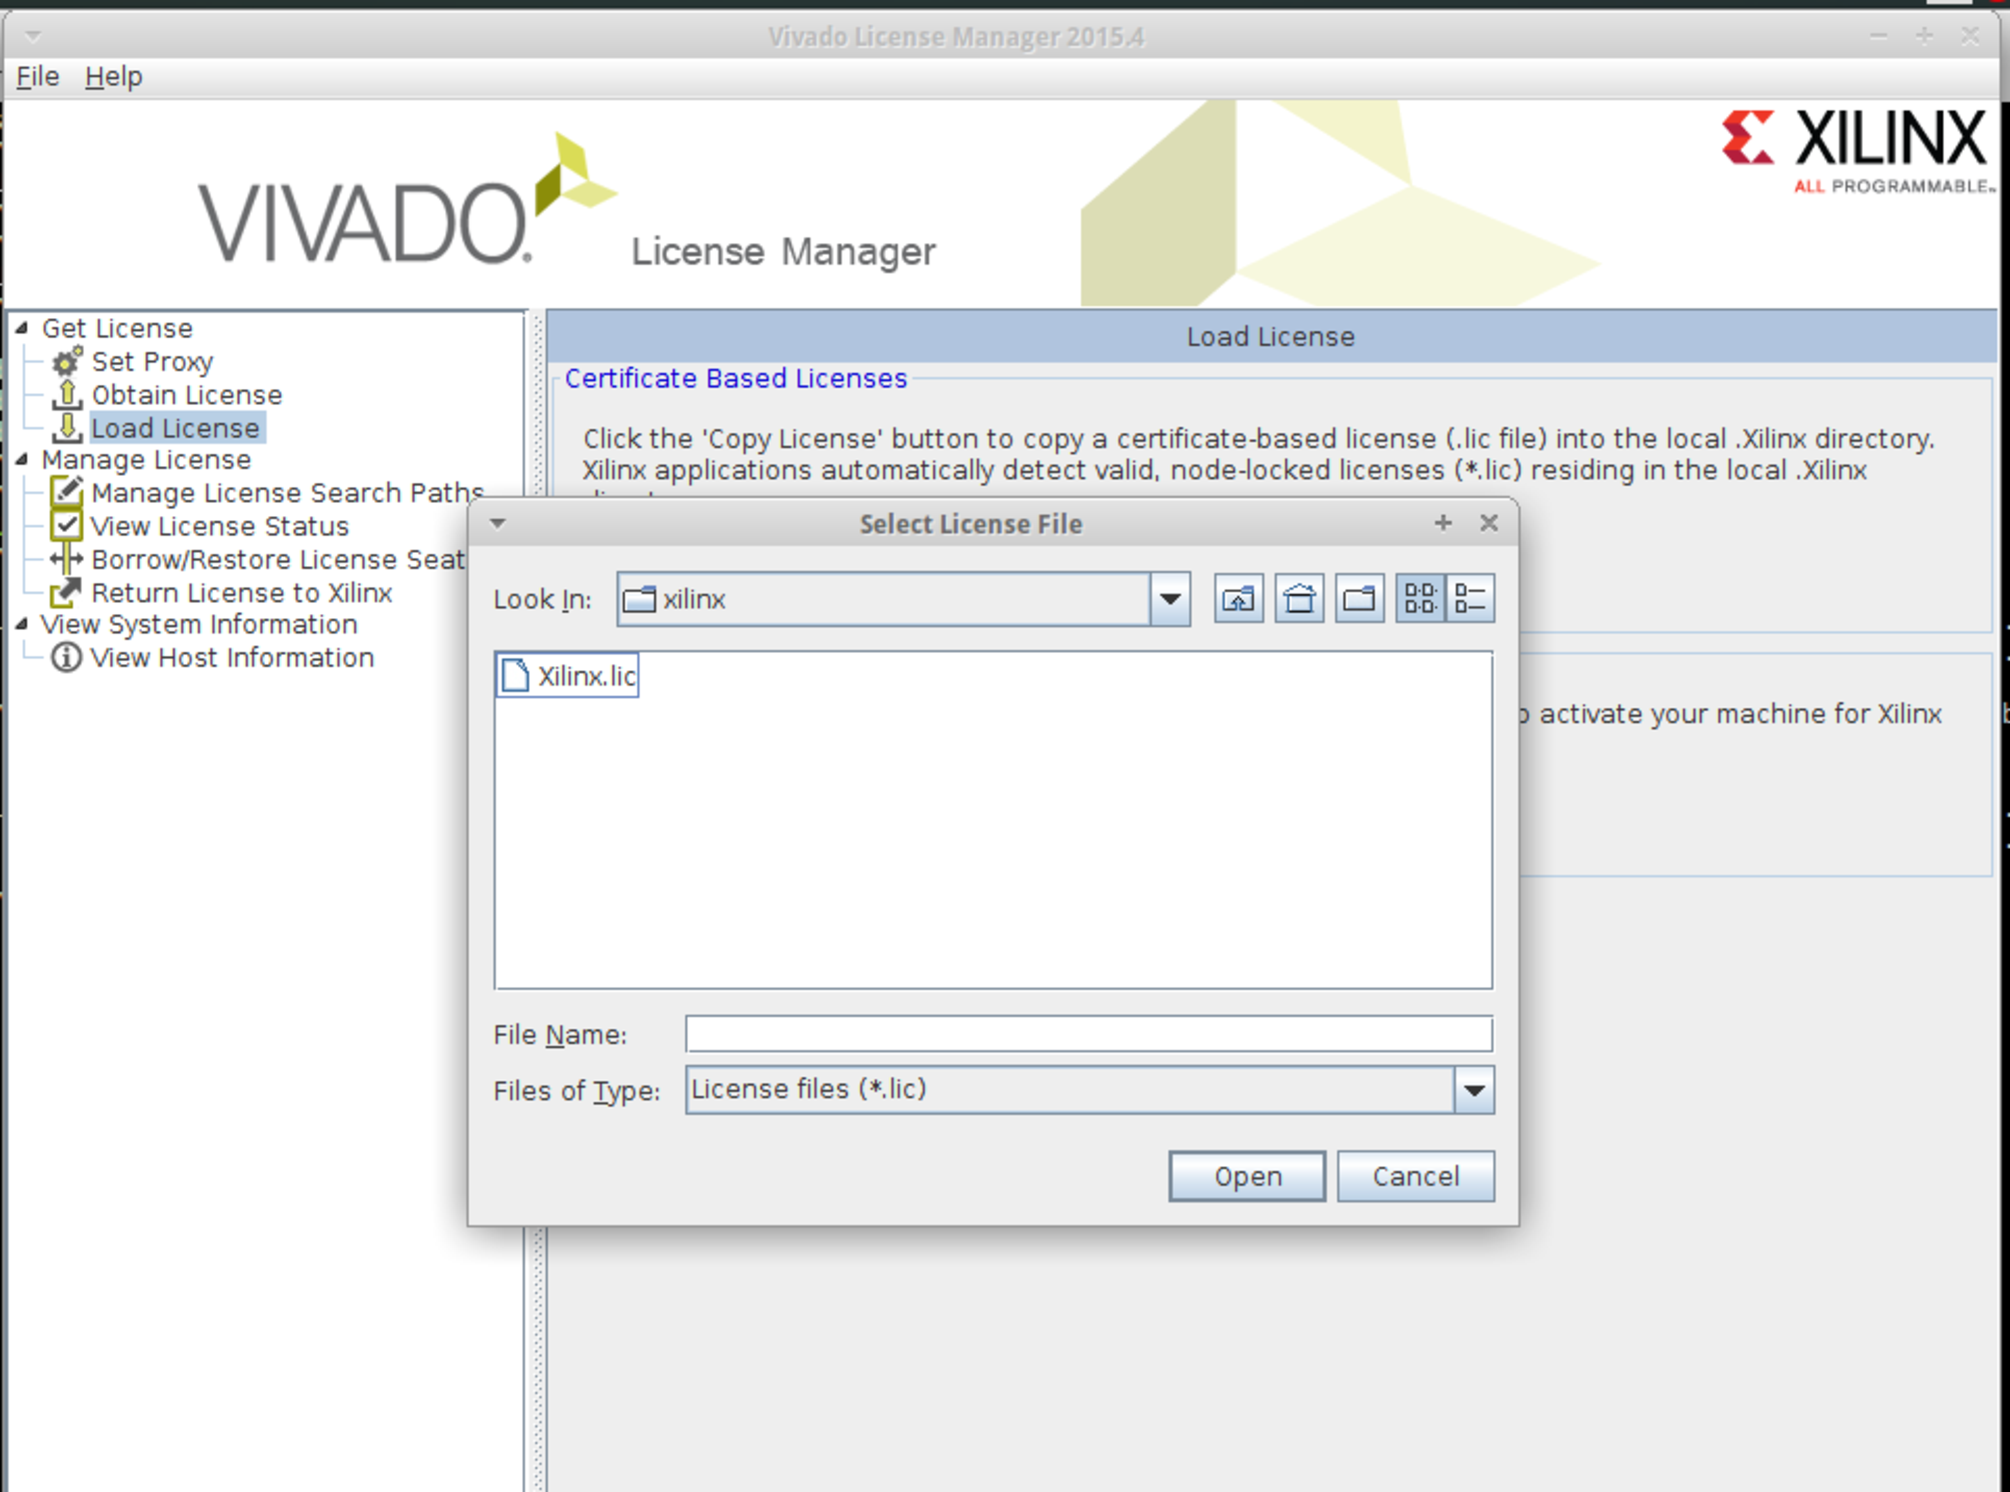
\includegraphics[height=8cm,width=12cm]{vivado_installer_12}
    \end{center}

    \begin{center}
    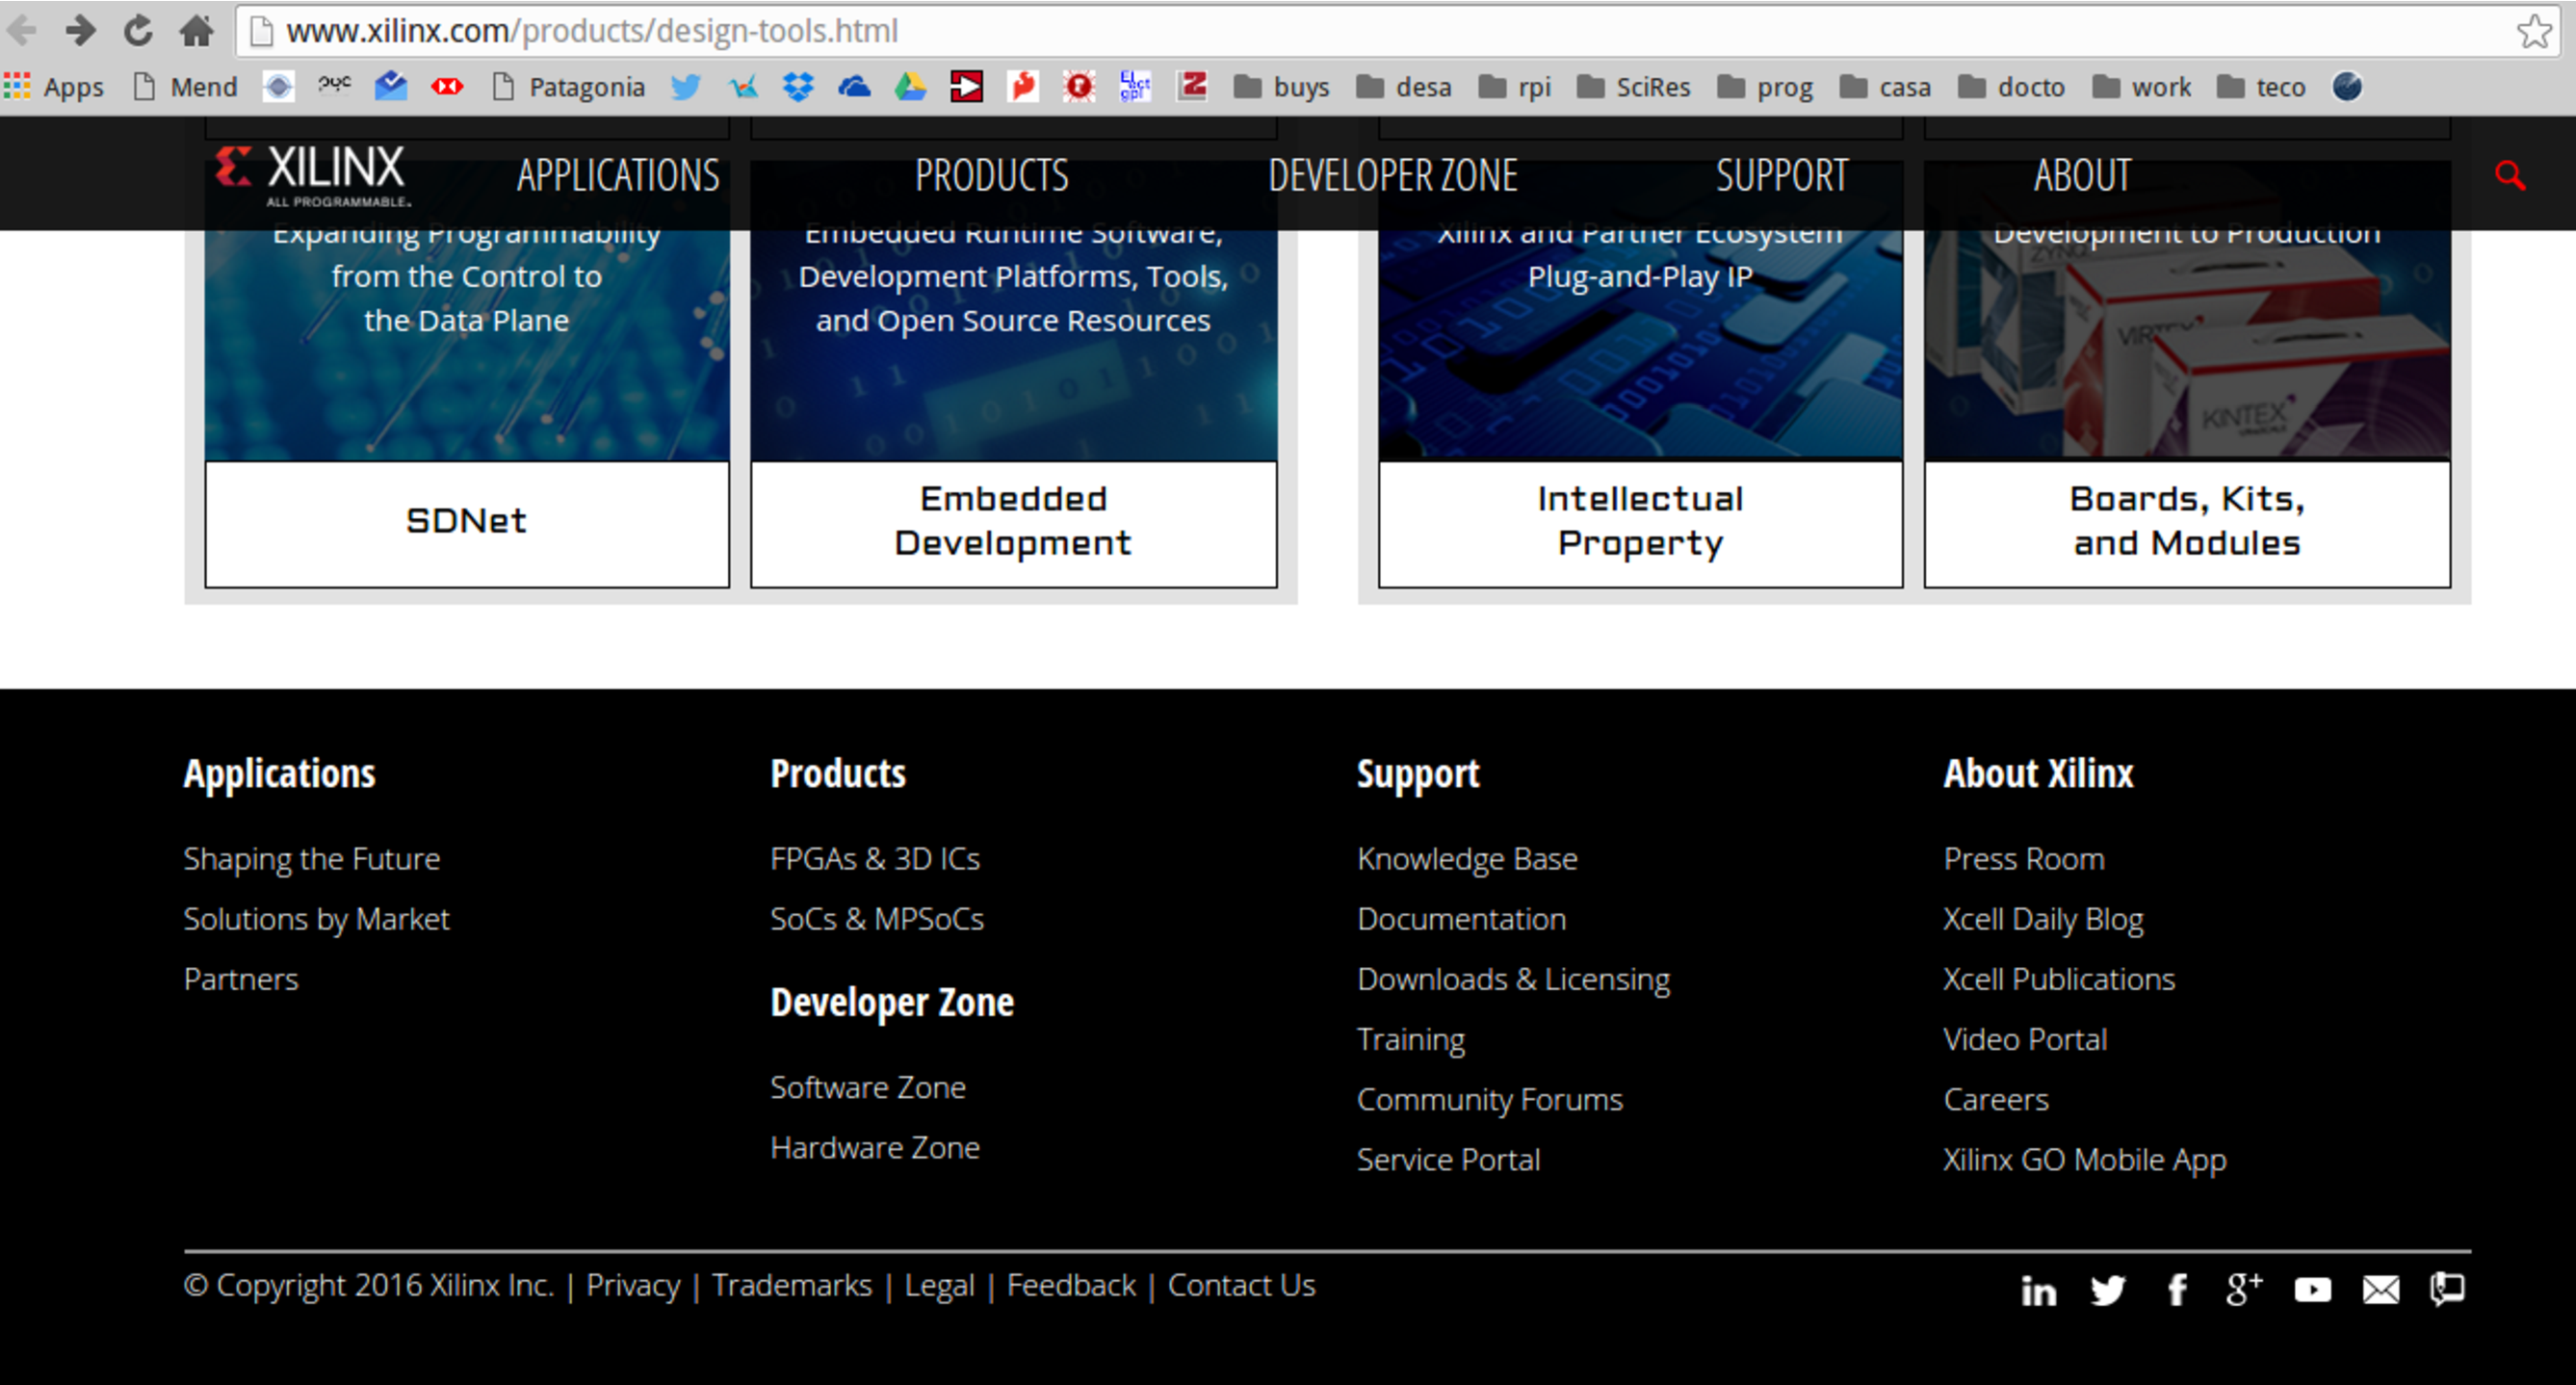
\includegraphics[height=8cm,width=12cm]{vivado_installer_13}
    \end{center}

    \begin{center}
    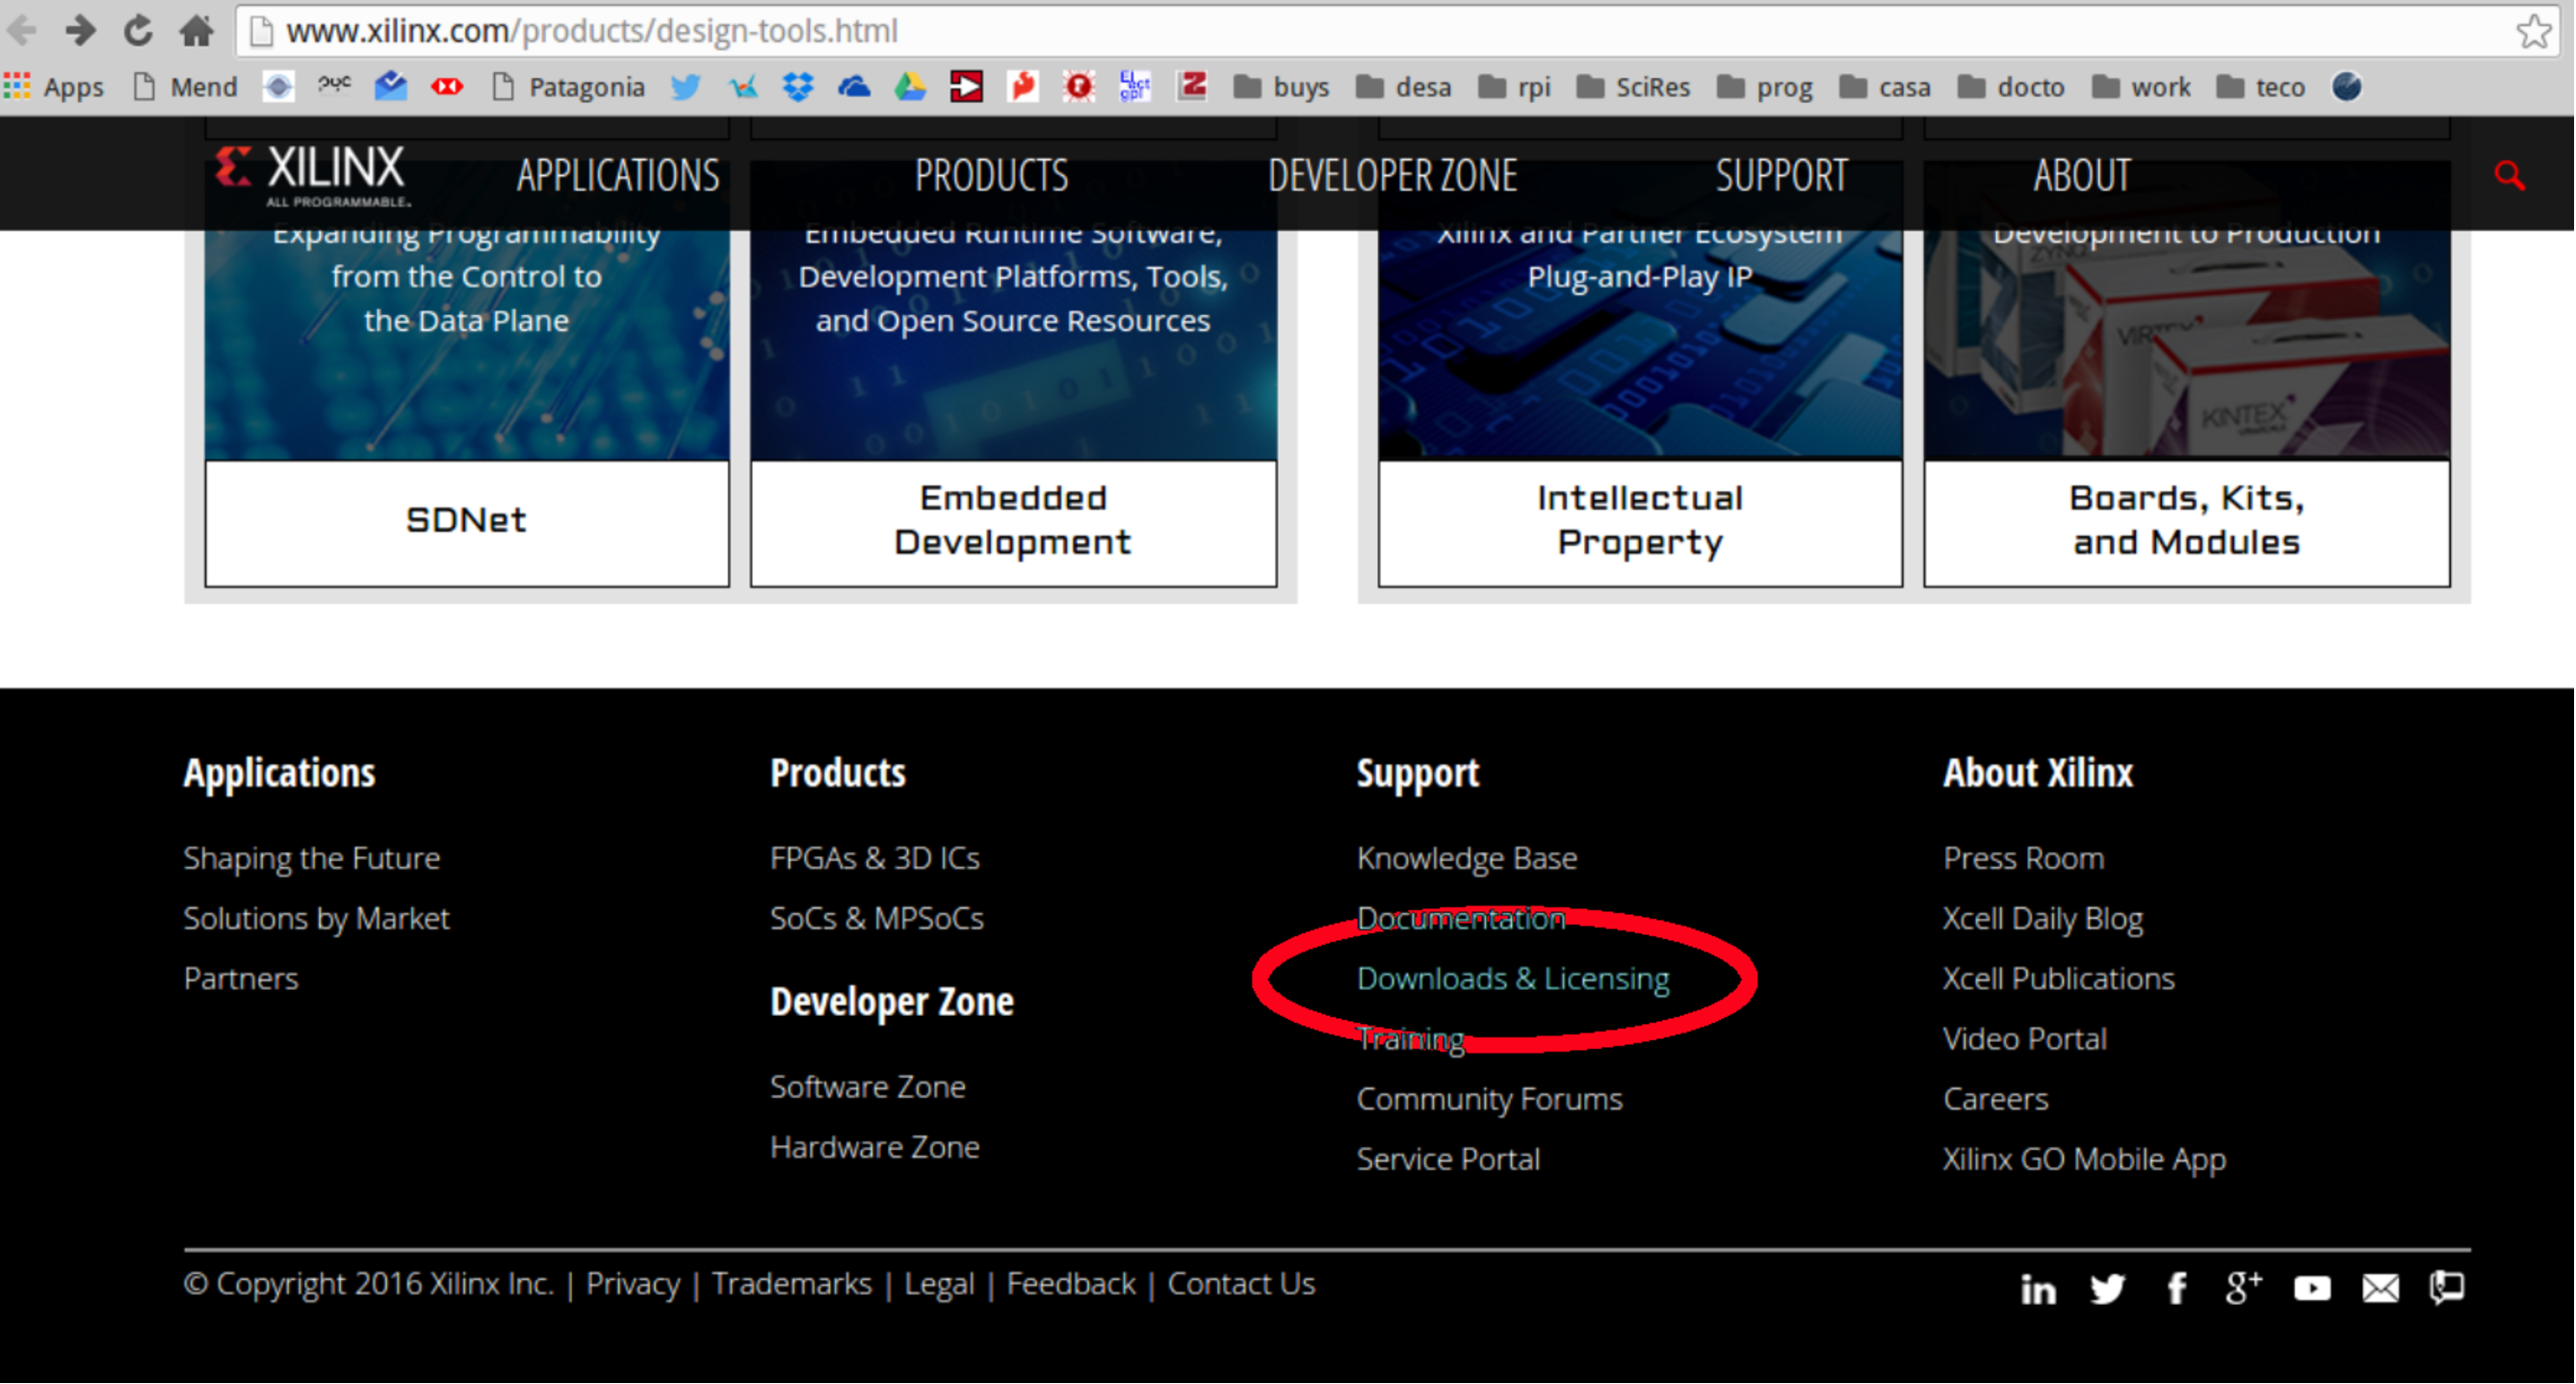
\includegraphics[height=8cm,width=12cm]{vivado_installer_13_bis}
    \end{center}

    \begin{center}
    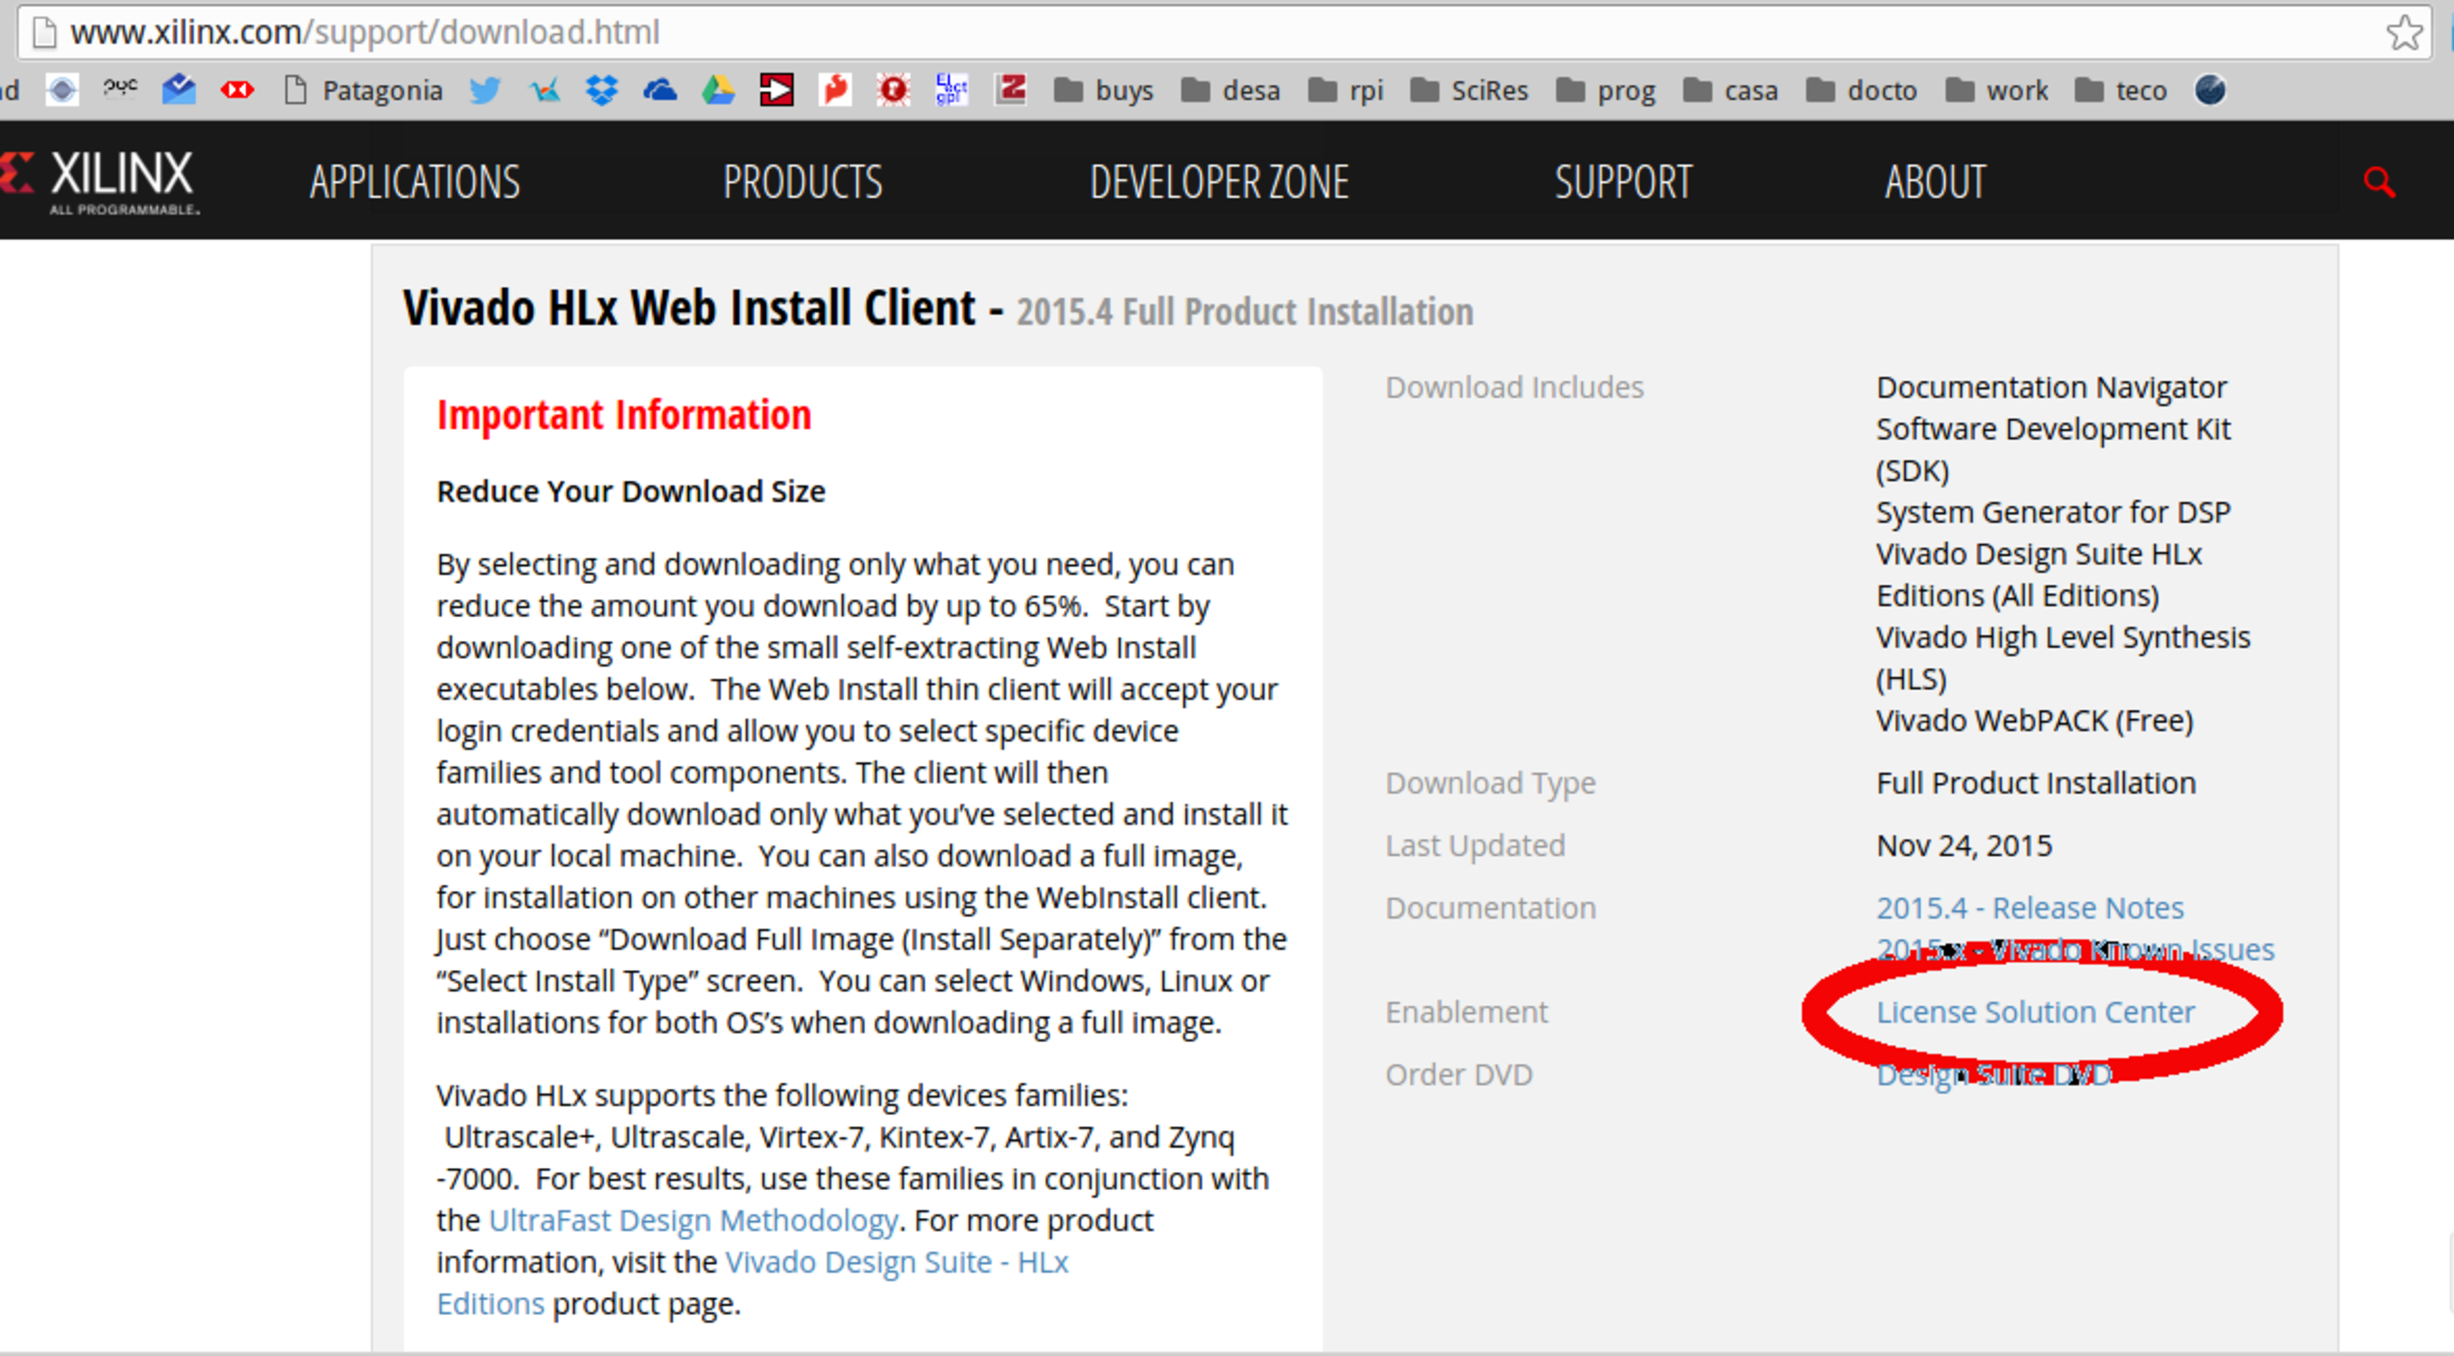
\includegraphics[height=8cm,width=12cm]{vivado_installer_14}
    \end{center}

    \begin{center}
    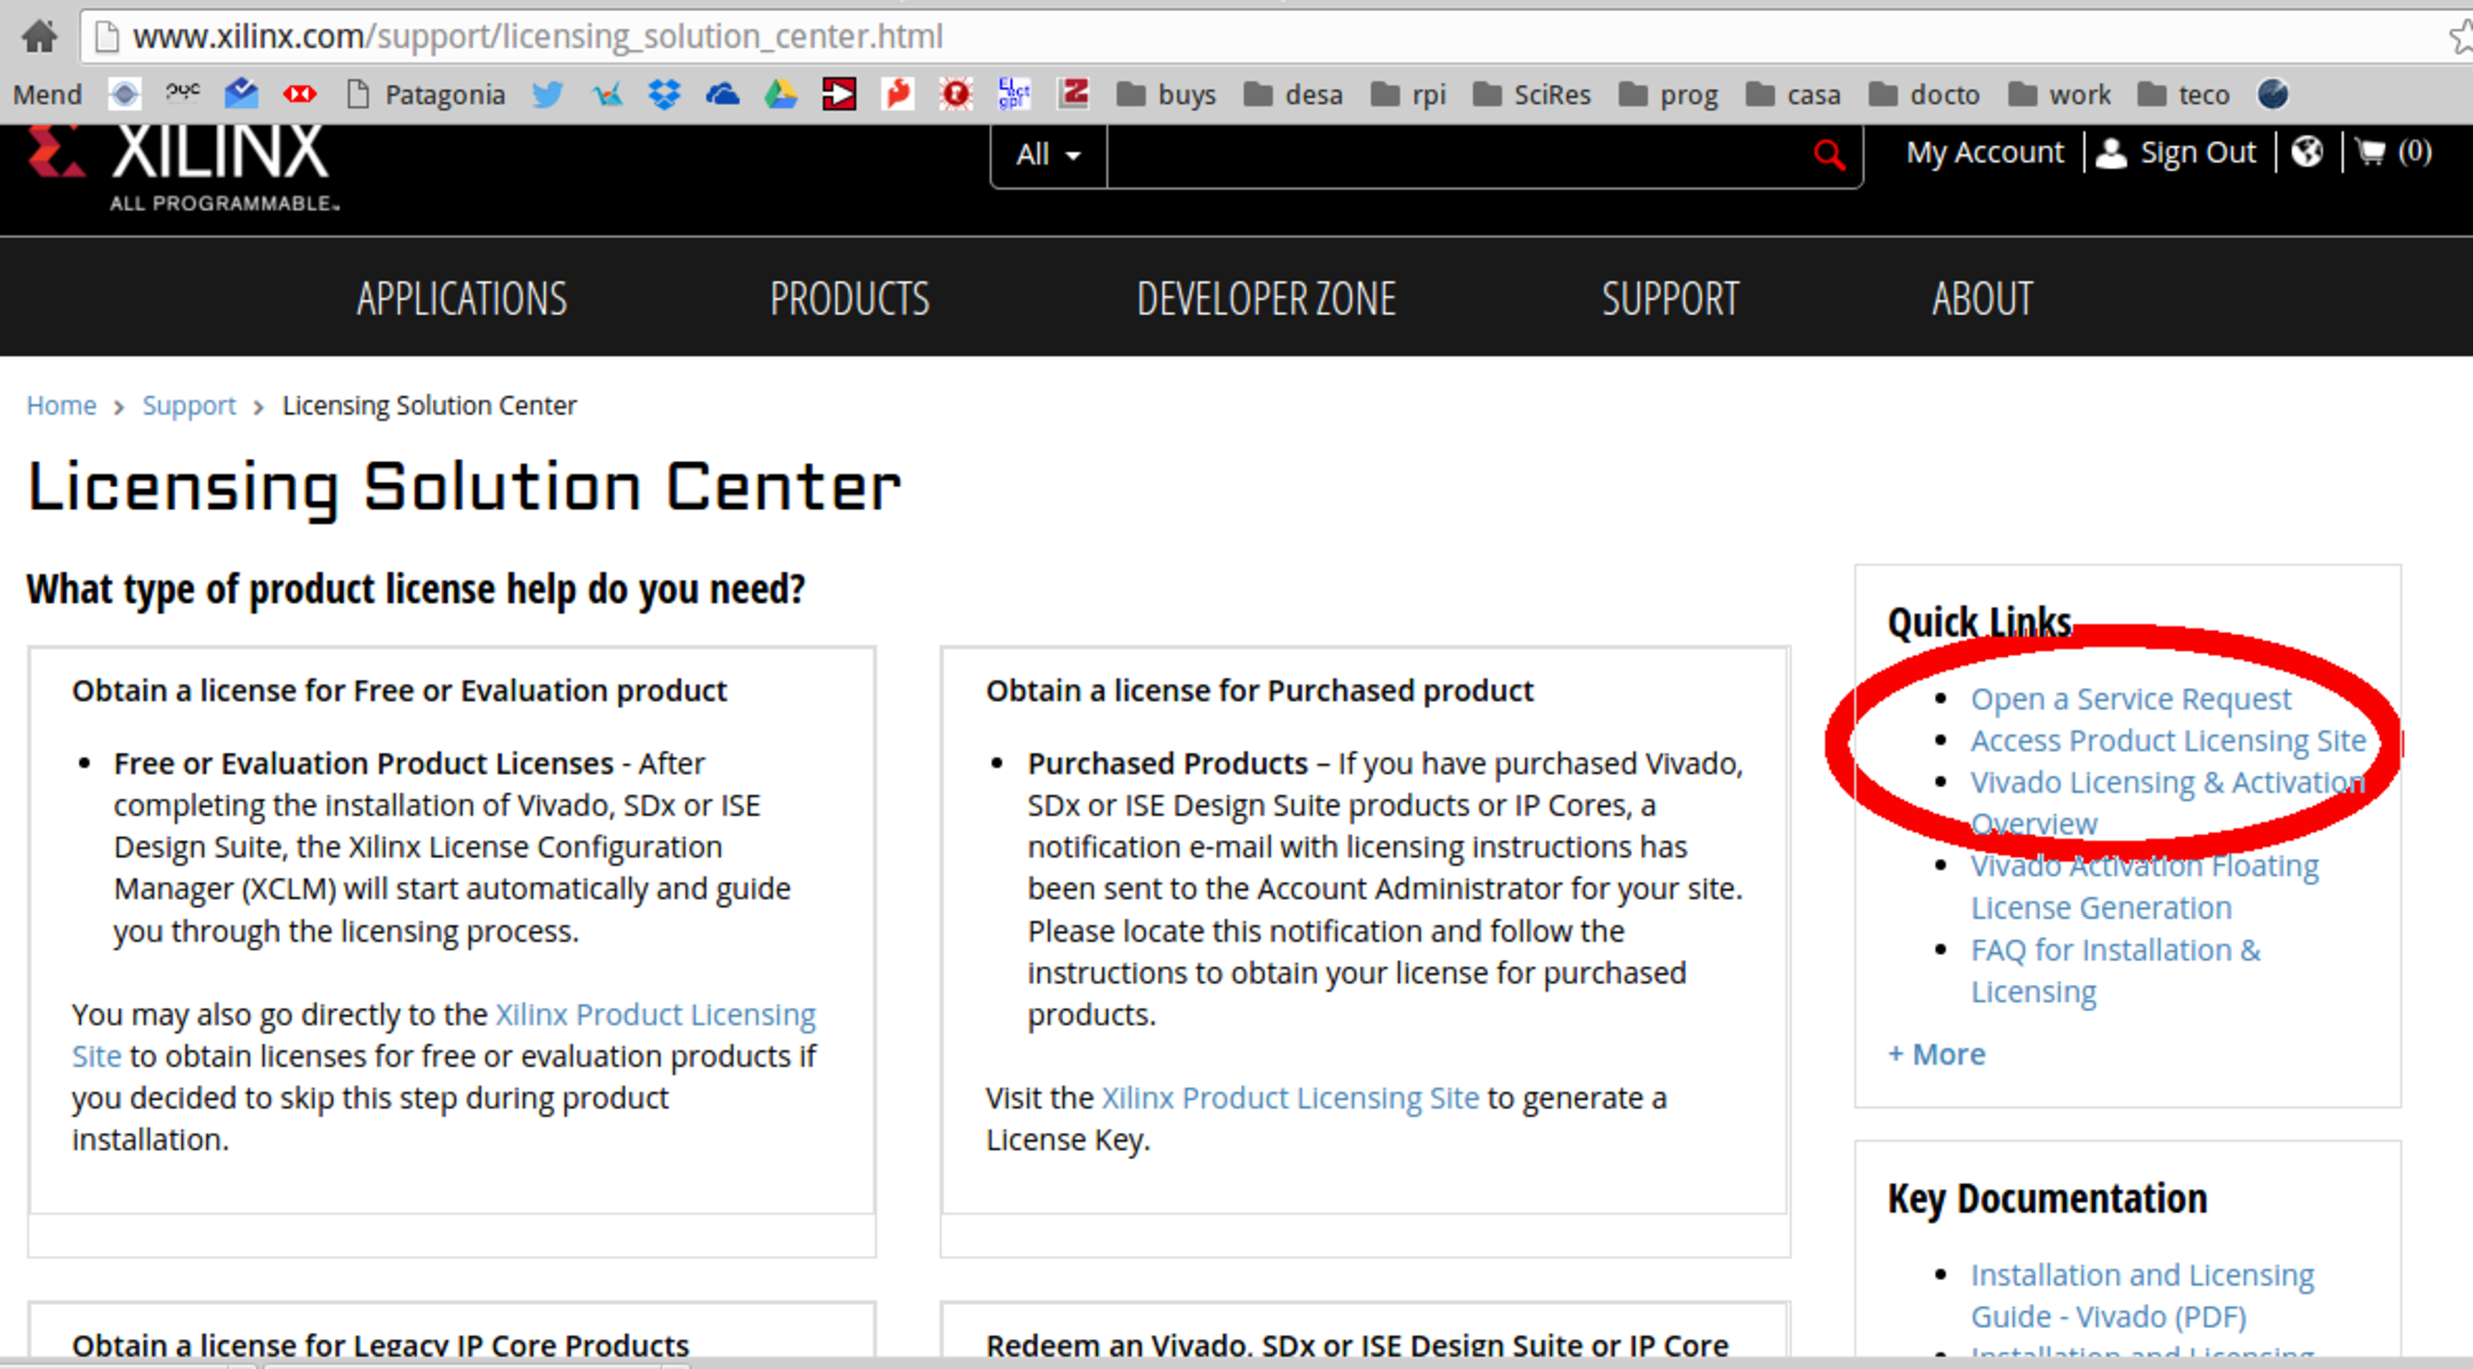
\includegraphics[height=8cm,width=12cm]{vivado_installer_15}
    \end{center}

    \begin{center}
    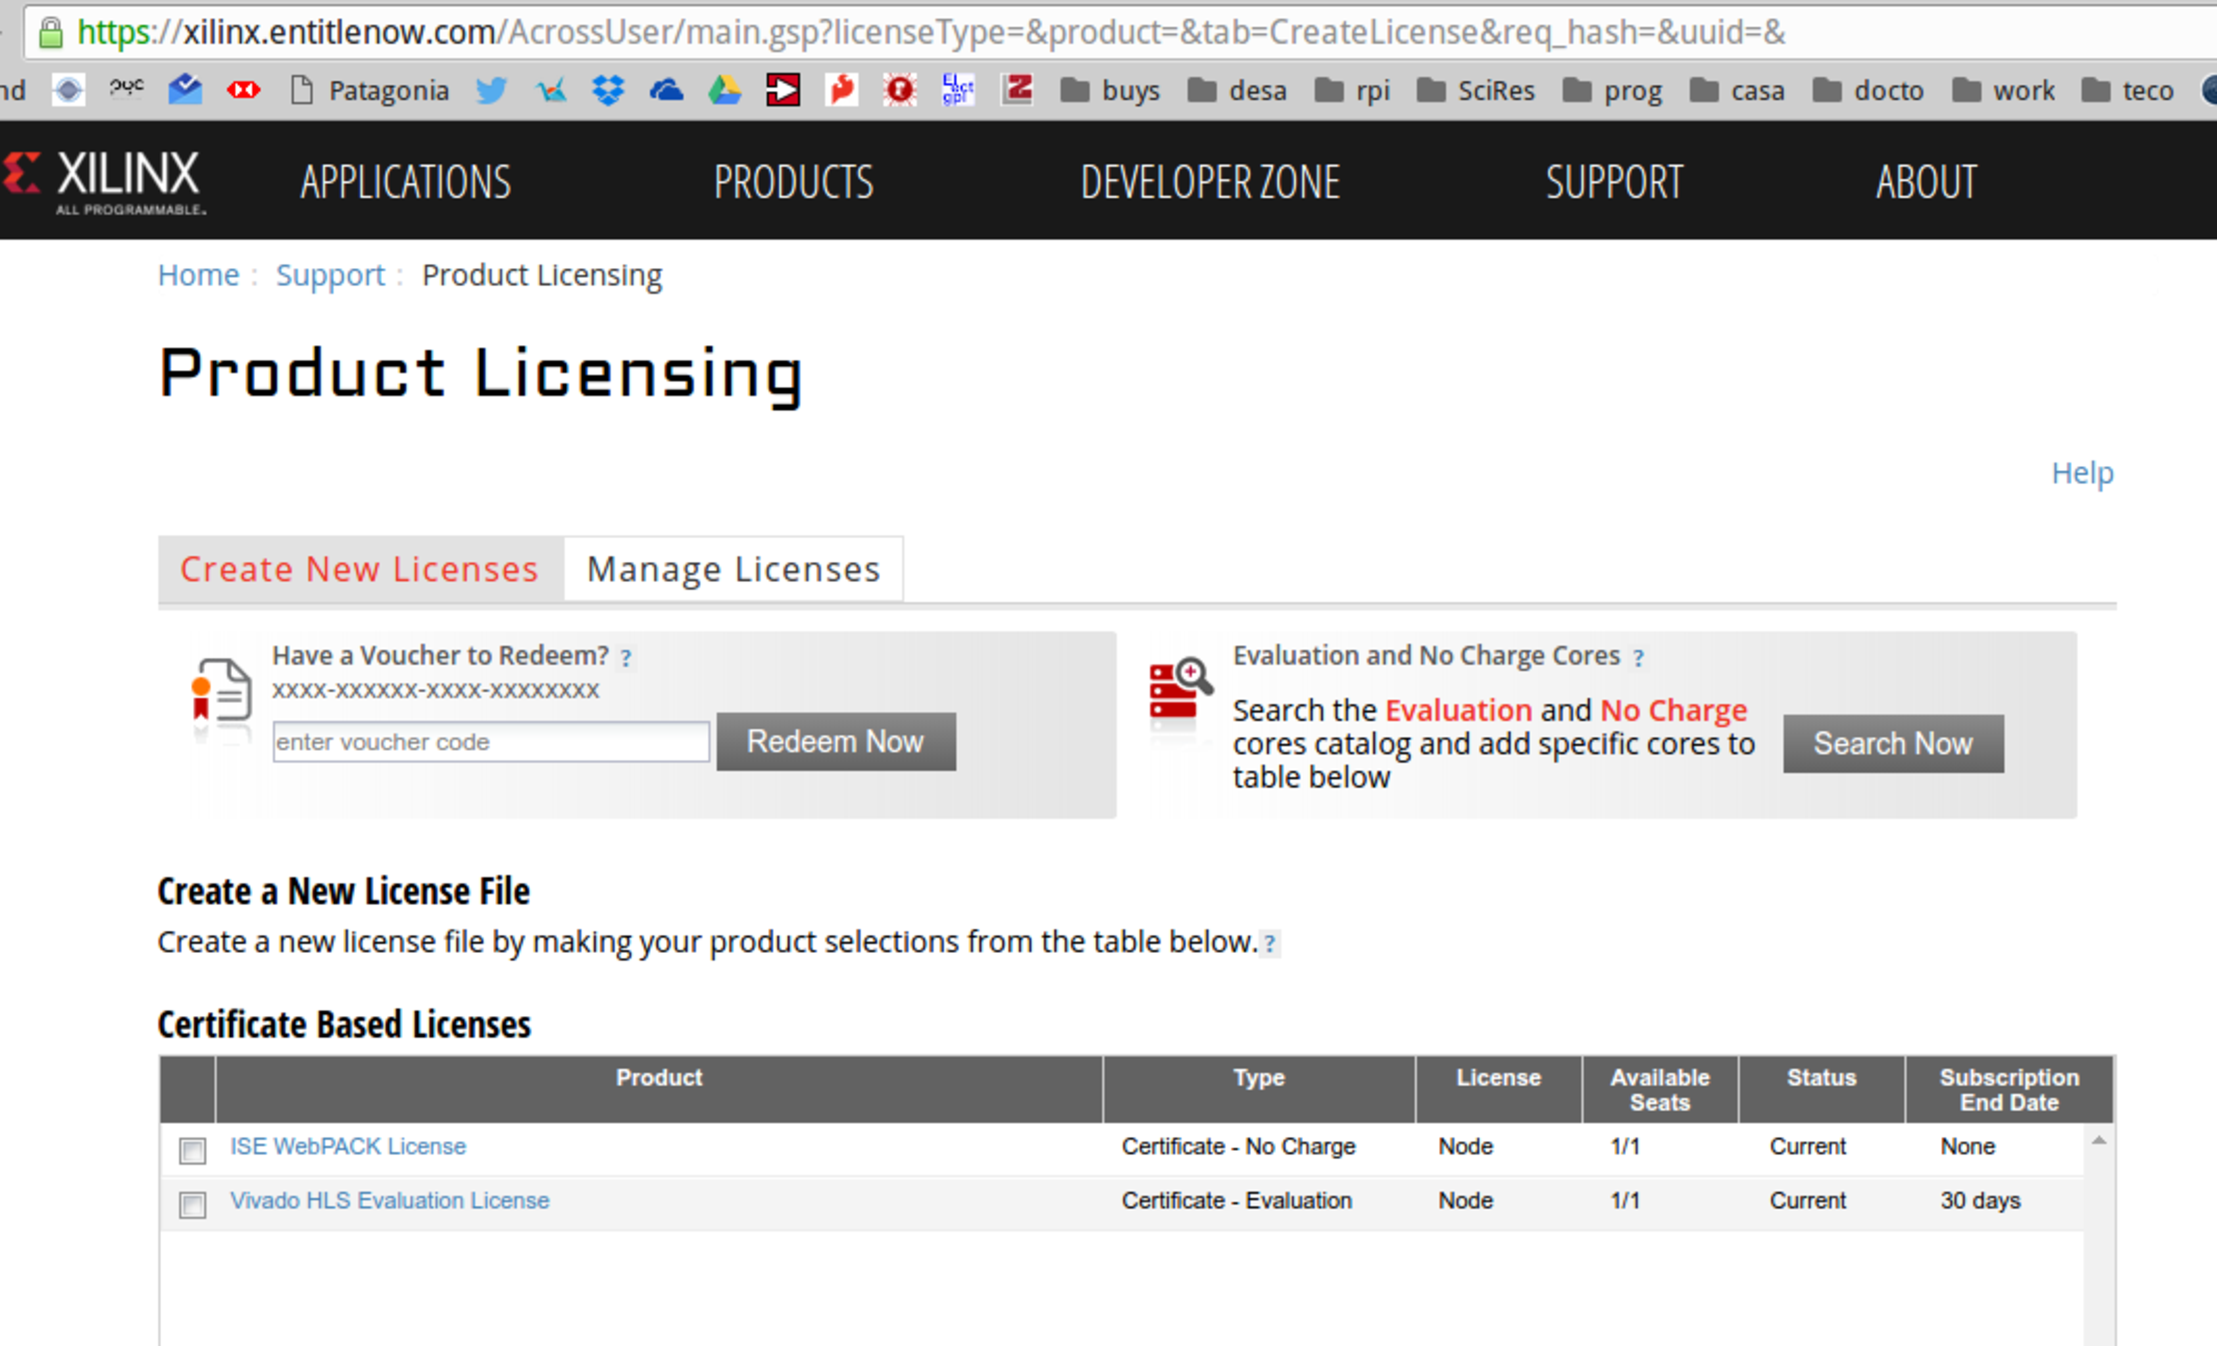
\includegraphics[height=8cm,width=12cm]{vivado_installer_16}
    \end{center}

\subsection{Completando la instalación}
\subsubsection{Pasos finales}
    Para terminar se deben cargar las variables de entorno que usará Vivado en
    su ejecución. Para esto existe el archivo
\texttt{/opt/Xilinx/Vivado/2015.4/settings64.sh}
\subsubsection{El archivo \textbf{settings64.sh}}
{\tiny{\texttt \#\#\#\#\#\#\#\#\#\#\#\#\#\#\#\#\#\#\#\#\#\#\#\#\#\#\#\#\#\#\#\#\#\#\#\#\#\#\#\#\#\#\#\#\#\#\#\#\#\#\#\#\#\#\#\#\#\#\#\#\#\#\\
      \# Copyright (c) 1986-2016 Xilinx, Inc.  All rights reserved. \#\\
      \#\#\#\#\#\#\#\#\#\#\#\#\#\#\#\#\#\#\#\#\#\#\#\#\#\#\#\#\#\#\#\#\#\#\#\#\#\#\#\#\#\#\#\#\#\#\#\#\#\#\#\#\#\#\#\#\#\#\#\#\#\#\\
      \vspace{4mm}
      source /opt/Xilinx/SDK/2015.4/.settings64-Software\_Development\_Kit.sh\\
      source
/opt/Xilinx/Vivado\_HLS/2015.4/.settings64-Vivado\_High\_Level\_Synthesis.sh\\
      source /opt/Xilinx/Vivado/2015.4/.settings64-Vivado.sh\\
      source /opt/Xilinx/DocNav/.settings64-DocNav.sh}}

\subsubsection{Configurando el ambiente Vivado}
    Antes de ejecutar cualquier código se deben cargar las variables de entorno:
    \begin{verbatim}
      source /opt/Xilinx/Vivado/2015.4/settings64.sh
    \end{verbatim}
    Una opción es incluir ese comando en el archivo \textbf{$\sim$/.bashrc}. De
esta
    forma, el sistema carga automáticamente las variables de entorno al inicio.

\begin{thebibliography}{9}

\bibitem{bibMinicom}
\href{https://es.wikipedia.org/wiki/Minicom}{Minicom}

\bibitem{bibGPSBee}
\href{http://wiki.seeedstudio.com/GPS\_Bee\_kit/}{Sensor GPSBee v1.2}

\bibitem{bibBMP180}
\href{https://www.adafruit.com/product/1603}{Sensor de presión y temperatura
BMP180}

%\bibitem{bibGIT}
%\href{https://github.com/}{Repositorio GIT}
%\bibitem{bibAuger}
%\href{http://auger.org.ar}{\emph{Observatorio Pierre Auger}}
%\href{www.auger.org.ar}{\emph{The Pierre Auger Observatory}}

\end{thebibliography}
\end{document}
